\documentclass[12pt,french]{report}
\usepackage[utf8]{inputenc}
\usepackage{graphicx}
\usepackage{epigraph}
\usepackage[dvipsnames]{xcolor}
\usepackage{babel}
\usepackage[font=small,labelfont=bf]{caption}
\sffamily
\usepackage{cite}
\usepackage{hyperref}
\hypersetup{
    colorlinks=true,
    linkcolor=magenta,
    filecolor=magenta,
    urlcolor=magenta,
    citecolor=magenta,
}
\usepackage[sfdefault,book]{FiraSans} %% option 'sfdefault' activates Fira Sans as the default text font
\usepackage[T1]{fontenc}
\usepackage{titlesec}
\titleformat{\chapter}[display]{\normalfont\bfseries}{}{0pt}{\Huge}\renewcommand*\oldstylenums[1]{{\firaoldstyle #1}}\setcounter{secnumdepth}{3}
\setlength{\parskip}{1em}
\usepackage{fontawesome}
\usepackage[toc,page]{appendix}
\usepackage{pdfpages}
\usepackage{float}
\usepackage{amsmath}

\title{Perception chimique chez la larve de poisson zèbre}
\author{Benjamin Gallois}

\begin{document}
\maketitle
\chapter*{Abstract}

\chapter*{Dedication}

\chapter*{Acknowledgements}

\tableofcontents

\part{FastTrack}
\chapter{Introduction}

  \epigraph{Talk is cheap. Show me the code.}{Linux Torvald}

	\section{Video based tracking}
    The tracking of objects from video recordings is a problem that has gained much popularity in recent years. It is mostly due to its great potential, both in academics and for commercial and security applications. Examples include autonomous cars that can drive themselves or the Airbus ATTOL project \cite{ATTOL} that allows fully automated take-off, landing, and taxiing based solely on image analysis. A large part of the research effort is focused on creating pedestrian recognition and tracking algorithms to automate the analysis of video surveillance data. Tracking is also widely used in the field of cinema and special effects (VFX), whether to stabilize shots or to realize special effects (e.g., motion capture). In this case, automated tracking on images allows reducing costs and production time. In science, the use of automated tracking, especially in biology and ecology \cite{dell2014automated}, is a rapidly growing field. It avoids the need to invasively mark animals and thus disturbing them. It allows generating a large amount of reliable data, reducing bias, and avoiding a long and laborious manual analysis.

    Object tracking can be separated into two categories: the Single Object Tracking (SOT), where the goal is to detect a single object in a more or less complicated scene, and the Multiple Object Tracking (MOT), where the goal is to detect and track several objects. In this dissertation, we will place ourselves within the MOT framework because it regroups the vast majority of scientific applications. In a scientific experiment, the tracking problem's difficulty is reduced by designing the setup well. In general, the image quality is good, the camera is fixed, and we can optimize the lighting to facilitate object detection. On the other hand, the tolerance to errors is low if one wants to produce reliable data and robust scientific conclusions. A decisive point is the algorithm's performance, which must analyze the data in a reasonable time compared to their production rate and meet the user's material and technical constraints. The ease of installation and use of the software that integrates the algorithm should not be neglected. The users brought to use these software are generally not experts in computer science and image analysis, and the software must be readily installable and usable by all.

    We will first see how tracking is a complex problem and how we can reduce or bypass this complexity. We will then present a non-exhaustive list of existing tracking software applied to diverse scientific fields. Finally, we will see how FastTrack's approach, the software we have created to solve the tracking problem, is different, and in which cases it can be useful.

	\section{The tracking, a not so simple problem}
    The image-based tracking of objects rest on three key steps: the acquisition of the images, which, depending on the acquisition parameters, will condition the difficulty of the tracking and the type of algorithm that can be used; the detection of objects, which consists in separating the objects from the background; and finally the assignment of objects from one image to another allowing to keep track of the objects' identities. Object tracking is generally a complex image processing task \cite{dell2014automated}. Depending on the objects studied, each step can be difficult. For example, animals are highly deformable objects interacting with each other, making the detection step complex. The scene can be complicated, with objects disappearing behind the decor elements, superimposing each other (the so-called occlusion phenomenon), or entering and leaving the field of view, complicating the detection and the association step.

    Object detection problems can usually be circumvented by the design of the experimental setup whenever it is possible. A fixed point of view and lighting optimization usually allow simple detection by subtracting a background image (without objects) and applying a threshold. For more complicated cases, a wide variety of algorithms are available \cite{yilmaz2006object} and applicable depending on the images' quality. The most common is to detect points of interest in the object. This technique is invariant to the point of view and illumination but requires a good image quality. Segmentation allows to separate the image by area of similarities and thus to detect objects of interest, many algorithms and approaches exist to segment an image. Machine learning can also be applied for objects detection \cite{zhao2019object}.

    Two main classes of algorithms can be distinguished to mitigate association problems. The first class of algorithms uses the object's kinematic quantities, such as direction or position \cite{qian2016effective}, to predict or find the position of the object on the next image and thus keep its identity. This method's error rate remains constant when we increase the number of individuals (keeping the density of objects fixed). It is generally fast, and this makes it a good candidate for real-time tracking applications. The major disadvantage of this approach comes from the error propagation phenomenon. If the algorithm makes an error in the assignment, it has no way to correct the error at the next step, and it propagates to the end of the analysis.
    The second class of algorithms is based on recognizing the object's points of interest, allowing the creation of a "fingerprint" unique to each object. That can be done using either a classical method \cite{perez2014idtracker, bai2018automatic}, or using machine learning \cite{mathis2018deeplabcut, romero2019idtracker}. This technique solves the propagation of errors problem and allows objects to be tracked over time, i.e., across several unpaired videos. For example, an animal can be recognized from one day of experiments to the next, which can be very useful, especially for behavioral studies. This method requires an image of sufficient quality to extract markers representative of the object. It also requires more computational resources, thus, an analysis that cannot be done in real-time. However, the main limitation is the number of objects it can track. It is currently limited to about ten objects per image with classical methods before the algorithms' performance degrades significantly. The machine learning approach makes it possible to increase the number of objects at the cost of long computation time and the need to use high-performance computers.

	\section{Existing software}
	\section{Existing software}
    Many tracking software already exist. We will make a non-exhaustive list of the most popular ones, separating them into two categories: proprietary software and open-source software.

    \subsection{Proprietary software}
    The proprietary software presented here are closed-source. The user cannot modify the code to adapt the software to his project or check precisely how the tracking is performed. On the other hand, they do not require any computer knowledge and benefit from a support service convenient for users that do not have a lot of computer knowledge. They are an excellent alternative to other options that are sometimes difficult to implement, but their high price can be a hindrance for some users.

    \paragraph{EthoVision XT}
    EthoVision XT is a software developed by the company Noldus. It accompanies the user from the acquisition of images, thanks to a system of experiment templates, to the data analysis with a module allowing to visualize standard behavioral parameters. The software is complete and widely used. It is somewhat specialized in the field of behavioral neurosciences. It includes modules for classical behavioral experiments (e.g., water-maze, rats social interaction). It also allows performing live tracking so that users do not have to save images for long experiments.

    EthoVision XT is a mature software. A large number of modules are available as well as a system that allows the user to create its own experiment template. The most significant disadvantage is that the user cannot modify the software or control how the tracking is done. Price can be a barrier for some users, as the software costs a minimum of 5,850 USD without modules, and it is compatible only with Windows. Focused on tracking animals, it will not be suitable for other systems.

    \paragraph{Any-maze}
    Any-maze is a software developed by Stoelting Co. It is specialized in the analysis of behavioral neuroscience experiments. It directly integrates tools for standardized tests (e.g., forced swim test, fear conditioning test), allowing fully automated analysis of these experiments. It can track in real-time or from recorded videos.

    Any-maze is a complete solution for creating and analyzing typical behavioral experiments. It can be purchased with the experimental setup already optimized and calibrated for the software. The Any-maze suite consists of three software packages. The tracking part is available for USD 6,495 or USD 1,500 per year. The software is available for Windows only.

    \paragraph{ToxTrack}
    ToxTrack \cite{rodriguez2018toxtrac} is a software that implements in a graphical interface the ToxId algorithm \cite{rodriguez2017toxid}. To summarize, the algorithm extracts objects from the background by applying a threshold. The pieces of trajectories between occlusions are divided into short and long trajectories based on a user-defined threshold time. A group of long trajectories where all individuals are observed simultaneously is then extracted. In this case, the assignment is made using the Hungarian algorithm Figure~\ref{appendix_hung}. The remaining trajectories are then assigned to the corresponding object selecting the best correlation value in a trajectory identification matrix Figure~\ref{part_1:toxId}. This matrix contains the similarity between every two trajectory fragments based on objects' features.
    The authors report that ToxId is as powerful as existing software, speedy, and can track objects in real-time. A disadvantage that can be seen in this algorithm is that it only works for a constant number of animals. The algorithm's initialization requires to have at one moment $t$ all the objects to be tracked simultaneously detectable for a user-defined time $t+dt$. The user-interface (UI) is sometimes difficult to use: the integrated tracking reviewer does not permit to correct the tracking or to replay the tracking frame by frame.

    The UI includes tools to define areas of interest as well as statistical analysis of the collected data. The software is only available for Windows. The project initially open-source change to a closed-source model, but the software is still under development.

    \begin{figure}[h]
    \centering
    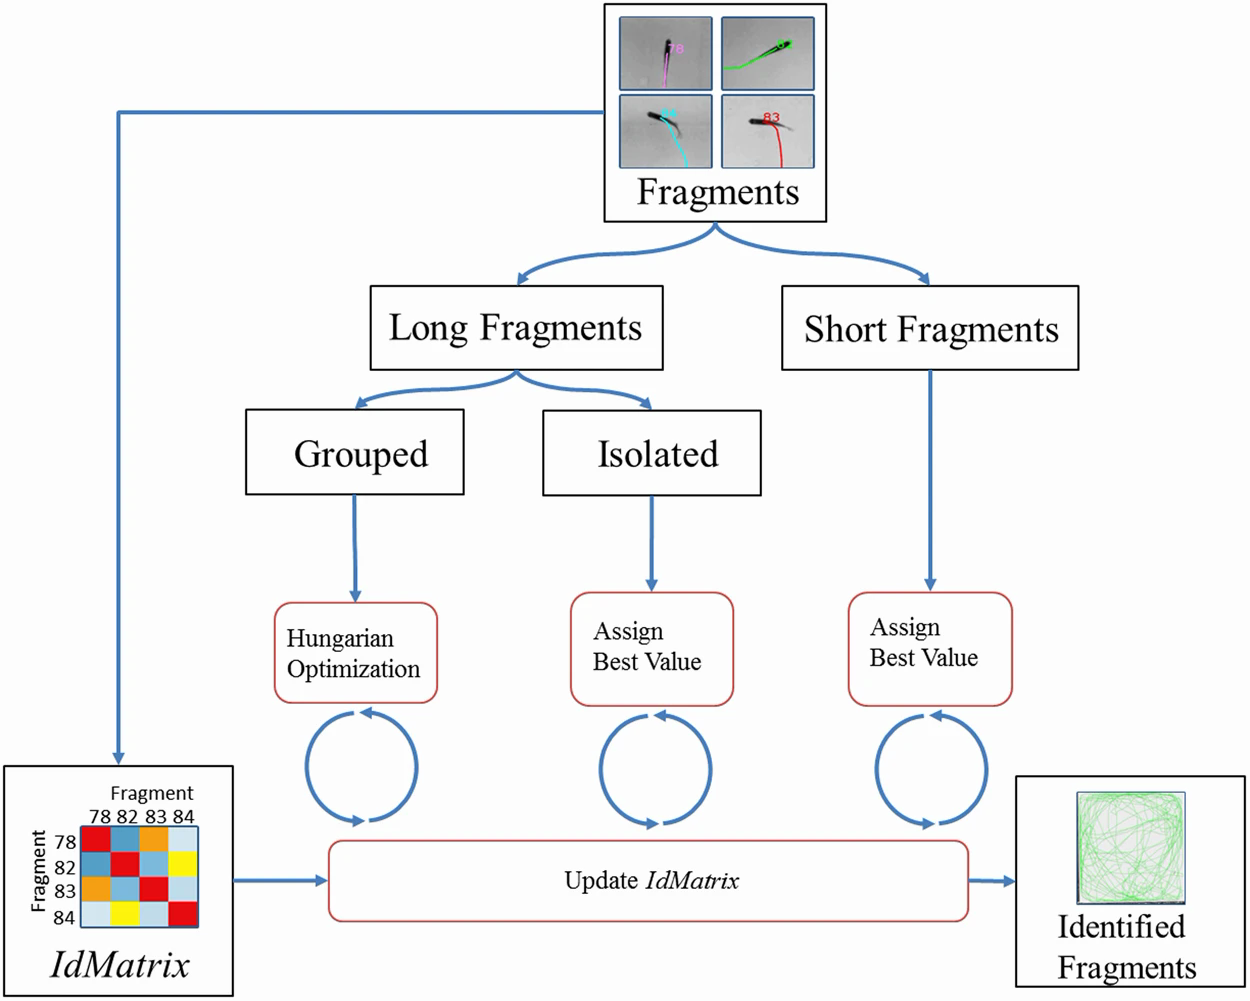
\includegraphics[width=0.75\textwidth]{part_1/assets/toxId.png}
    \caption{{\bf ToxId workflow chart.}}
    \label{part_1:toxId}
    \end{figure}

    \subsection{Open-source software}
    Open-source software allows the user to read, modify, and distribute the software. It is the preferred alternative to commercial software. From a scientific perspective, using open-source software increase transparency and lead to easier replicability of scientific results. From a development standpoint, it leads to better code quality and fewer bugs.
    In general, no individual assistance service is provided. The collaborative development of most of these software allows the user to report bugs and participate in their development to help the community.

    \paragraph{idTracker}
    IdTracker \cite{perez2014idtracker} is a MATLAB library that allows to track multiple objects in video recording. It is based on the extraction of a "fingerprint" for each object thus a reliable association without errors propagation. The advantage of idTracker is that it can recognize an object over several videos and after a relatively long time, which can be useful to track individuals' behavior over several series of experiments.

    IdTracker is solving amazingly well the propagation of errors problem during the association phase. However, it is limited by the number of objects it can track, currently about twenty, due to the movie's length necessary for extracting each object's "fingerprint". This task can go up to 30 minutes minimum for a high object density. The required image quality is an essential factor and must be at least 150 pixels per animal. The computation time is relatively long, in the order of 0.5 to 2 seconds per image, and requires a large RAM amount. The installation of idTracker can be done without the need to buy MATLAB thanks to the Matlab Run Time Compiler but only under Windows. Therefore, it is necessary to purchase a MATLAB license for other platforms and have minimal knowledge of the language to set up idTracker.

    \paragraph{DeepLabCut}
    DeepLabCut \cite{mathis2018deeplabcut} is a framework that solves the so-called "pose estimation" problem, which consists of finding an object and its position, or part of an object, in an image. It can be directly related to the SOT problem if the objects to be tracked are different, for example, a right mouse ear and a mouse nose, which can then be found on each image and then associated in the case where there is only one mouse. In the case of several similar objects to be found and associated from one image to another (MOT), this detection will have to be combined with an association step to obtain the tracking. Even if DeepLabCut answers a slightly different problem, it can, by its design, be coupled with an external association algorithm to make a tracking software.

    DeepLabCut is directly based on the feature detection algorithm of the DeeperCut framework \cite{insafutdinov2016deepercut}, specialized in the detection of human body movements. The authors of DeepLabCut have studied this algorithm's performance applied to the field of behavioral neuroscience, such as the detection of mice snouts or drosophila legs. They have added tools to train the algorithm easily and test its robustness.

    It takes advantage of deep learning to solve the so-called estimation pose problem. As a reminder, deep learning is a machine learning algorithm that consists of training a neural network containing several layers. In DeepLabCut, the network consists of several residual neural networks (ResNets) pre-trained on the ImageNet database. The network is then fine-tuned by training on images where the parts to be detected are annotated. In the end, the algorithm gives the probability of presence of the object in the image. The authors have shown that the performance is at least as good as human detection and can be obtained with very little training data (200 annotated images).

    DeepLabCut, as previously mentioned, is a framework, and despite an excellent documentation \cite{nath2019using}, it can be challenging to use it for a user with little computer skills. The installation process lasts from 10 to 60 minutes and requires a GPU installation to get the most out of the software. Besides, the algorithm requires a lot of computing power. To give an idea, images of 682x540 pixels, analyzed with a last-generation GPU, lead to an analysis speed of 30 frames per second. Without GPU, this time can be multiplied by a factor of 10 or 100 \cite{mathis2018inference}.

    We see that DeepLabCut is of great interest to find objects in an image with precision. It is particularly aimed at behavioral neuroscience, allowing complex movement tracking (e.g., hand fingers in a mouse). It will not be suitable for users with little computer knowledge interested in more extensive problems and with little data to process.

    \begin{figure}[h]
    \centering
    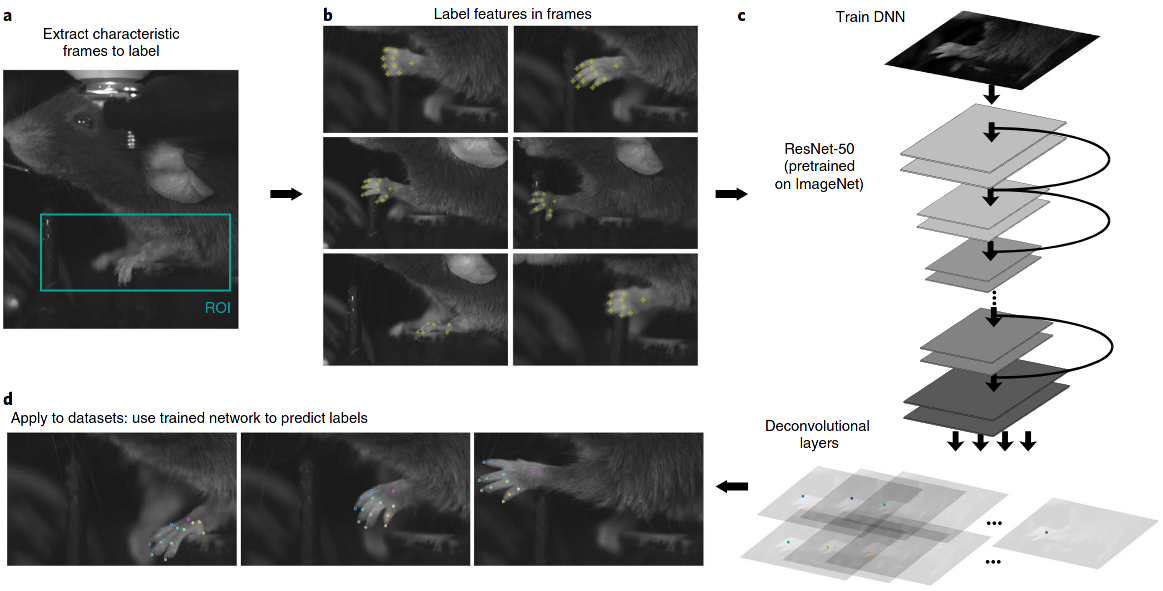
\includegraphics[width=0.75\textwidth]{part_1/assets/deeplabcut.png}
    \caption{{\bf DeepLabCut workflow chart.}}
    \label{part_1:deeplabcut}
    \end{figure}

    \paragraph{idTracker.ai}
    IdTracker.ai \cite{romero2019idtracker} is a framework that allows tracking animals with almost perfect accuracy. IdTracker.ai takes advantage of deep learning to carry out the association. In the first step, each object is segmented by applying a threshold. A convolutional network classifies each detected blob as containing a single object or several objects. Another convolutional network finds the identity of each individual throughout the movie.

    This system requires enough data to train the network that will recognize each individual. The authors found that robust tracking can be obtained with only thirty isolated images of each individual. Therefore, it is necessary to plan for a minimum of five hundred images for a dozen individuals with a minimum of twenty-five frames per second. A resolution of three hundred pixels per animal is recommended for good tracking accuracy. A limiting factor of idTracker.ai is that it requires a lot of computing time and a lot of RAM. The authors report about twenty minutes for processing a video with eight zebrafish and about six hours for a hundred zebrafish on about two thousand high definition images. Even if a UI is available to help the user, primary computer and programming knowledge is required, and suitable hardware. The use of a GPU is strongly recommended.

    This software is suitable for users who want perfect and fully automated tracking from high-quality videos having a powerful computer. A tool is integrated to review and correct the tracking, but the lack of ergonomy makes it sometimes difficult to use.

    \begin{figure}[h]
    \centering
    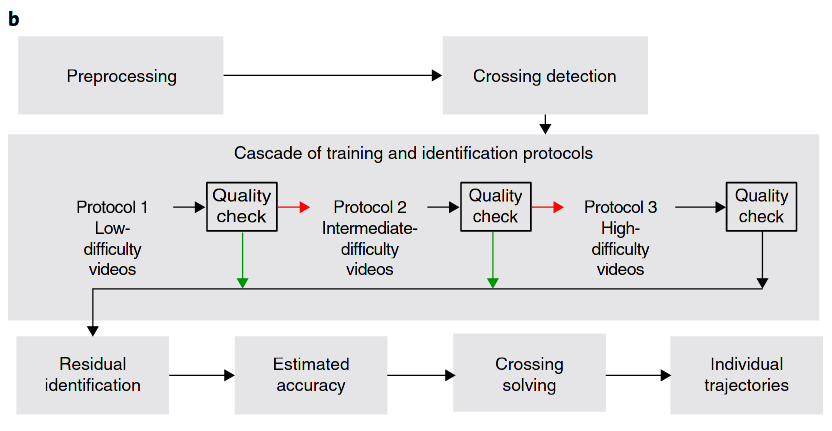
\includegraphics[width=0.75\textwidth]{part_1/assets/idtrackerai.png}
    \caption{{\bf IdTracker.ai workflow chart.}}
    \label{part_1:idtrackerai}
    \end{figure}

    \section{FastTrack: an original approach}
    We have previously listed the most used tracking software in different fields of science. We can see that a fast software requiring little computing power, versatile (i.e., that can be applied to any systems with a variable number of objects), easy to install, and open-source is missing.
    To fill this void, we designed a software called FastTrack. This software contains two distinct parts:
    \begin{itemize}
        \item An interface where standard image analysis procedures are implemented to detect objects, and a tracking algorithm that allows keeping the identity of objects from one image to another, fast and with a low error rate.
        \item An ergonomic interface where the tracking can be checked and and manually corrected if necessary.
    \end{itemize}
    We will notice here the difference in approach between FastTrack and existing software. Instead of developing a system that requires high computing power, which is slow but provides fully automated and highly reliable results, FastTrack implements a fast and easy to set up, very generalized method. The correction of the remaining errors is left to the user but can be done natively in the software, the ergonomic interface allowing a fast and efficient correction.
    This solution has several advantages, the first one being that it does not require any programming knowledge. Any user can perform a perfect analysis in a very short time. Moreover, it has been shown that the post-processing work can be estimated by an analysis of the geometrical and dynamic parameters of the studied system, which allows the user to know if the software is adapted to his needs. For many of the systems studied, the post-processing is only a quick check. If the number of occlusions is too high, and a perfect tracking accuracy is necessary without having to resort to manual correction, another solution must be considered.

    FastTrack is distributed under a free software license and implemented in a modular and fully documented manner. Each user can thus modify the software at his convenience or contribute to it. The tracking algorithm is decoupled from the detection and correction interface, which makes it extremely easy to integrate FastTrack into an existing project. The software is easily installed in less than 5 minutes and is compatible with Linux, macOS, and Windows. It can run on modest configurations and Single Board Computer (SBC) such as the Raspberry Pi.

\chapter{Design and implementation}

    \epigraph{Testing can only prove the presence of bugs, not their absence.}{Edsger W. Dijkstra}

    \section{Tools used}
    The choice of tools and libraries used in designing software is paramount, and several selection factors must be taken into account.
    The first criterion to consider is the license. We chose to put FastTrack under a free license (GPL3), which implies that the language used and the libraries must also be under compatible licenses. The choice of an open-source license is evident in the case of scientific software. The user can then check how the software works, change it to adapt it to his needs, and share it.
    The second criterion is to choose the libraries used carefully, considering the future of the software so that the developers do not have to change libraries if their capabilities prove insufficient as the software evolves. Mature libraries offering long-term support are preferred.

    In this perspective, FastTrack has been implemented in C++ using the Qt \cite{Qt} and OpenCV \cite{opencv_library} libraries for the graphical interface and image analysis, respectively. Unit tests are performed using the Google Test library.

    C++ is a computer language created by Bjarne Stroustrup in 1985. Offering high performance, it is standardized by the International Organization for Standardization (ISO). It is the language of choice for image analysis applications and the creation of complex graphical user interfaces.

    Qt is an open-source GUI library created by Haavard Nord and Eirik Chambe-Eng, two physicists, in 1991 when developing ultrasonic image analysis software. With extensive documentation and a large community, it is very mature. It allows creating graphical user interfaces for Linux, Mac, and Windows from the same source code.

    OpenCV is an open-source image analysis library created by Intel in 1999. Very complete and efficient, it has become the reference in image analysis for both academics and commercial applications.

    Google test is a suite for automating unit tests in C++. OpenCV notably uses it. The purpose of unit tests is to verify that each part of the program works as expected. This practice has several advantages: detecting more easily possible errors during the implementation of new features and facilitating software development when it grows in size to avoid any error inclusions. This series of tests are automatically performed on each new commit, see Section ~\ref{part_1:cicd}.

    \section{Implementation}
    FastTrack's operation can be divided into three parts: the detection of objects, the association of objects from one image to another, and finally, a correction step.

    Each analysis begins with the opening of an image sequence or a video file. The user can choose between two types of interfaces, an interactive interface where he can only open one film at a time. It allows the user to see, in real-time, the impact of parameters on the images, which facilitates the determination of the optimal analysis parameters. A second interface allows many movies to be opened simultaneously, either by giving a parameter file or selecting the parameters in the interface. It is useful when the user wants to analyze many movies for which he already knows the optimal analysis parameters.

    Both interfaces can be used in a complementary way. The user can find the optimal parameters with the interactive interface and then automate the analysis of many movies by tracking them in batches in the software.

    \begin{figure}[h!]
    \centering
    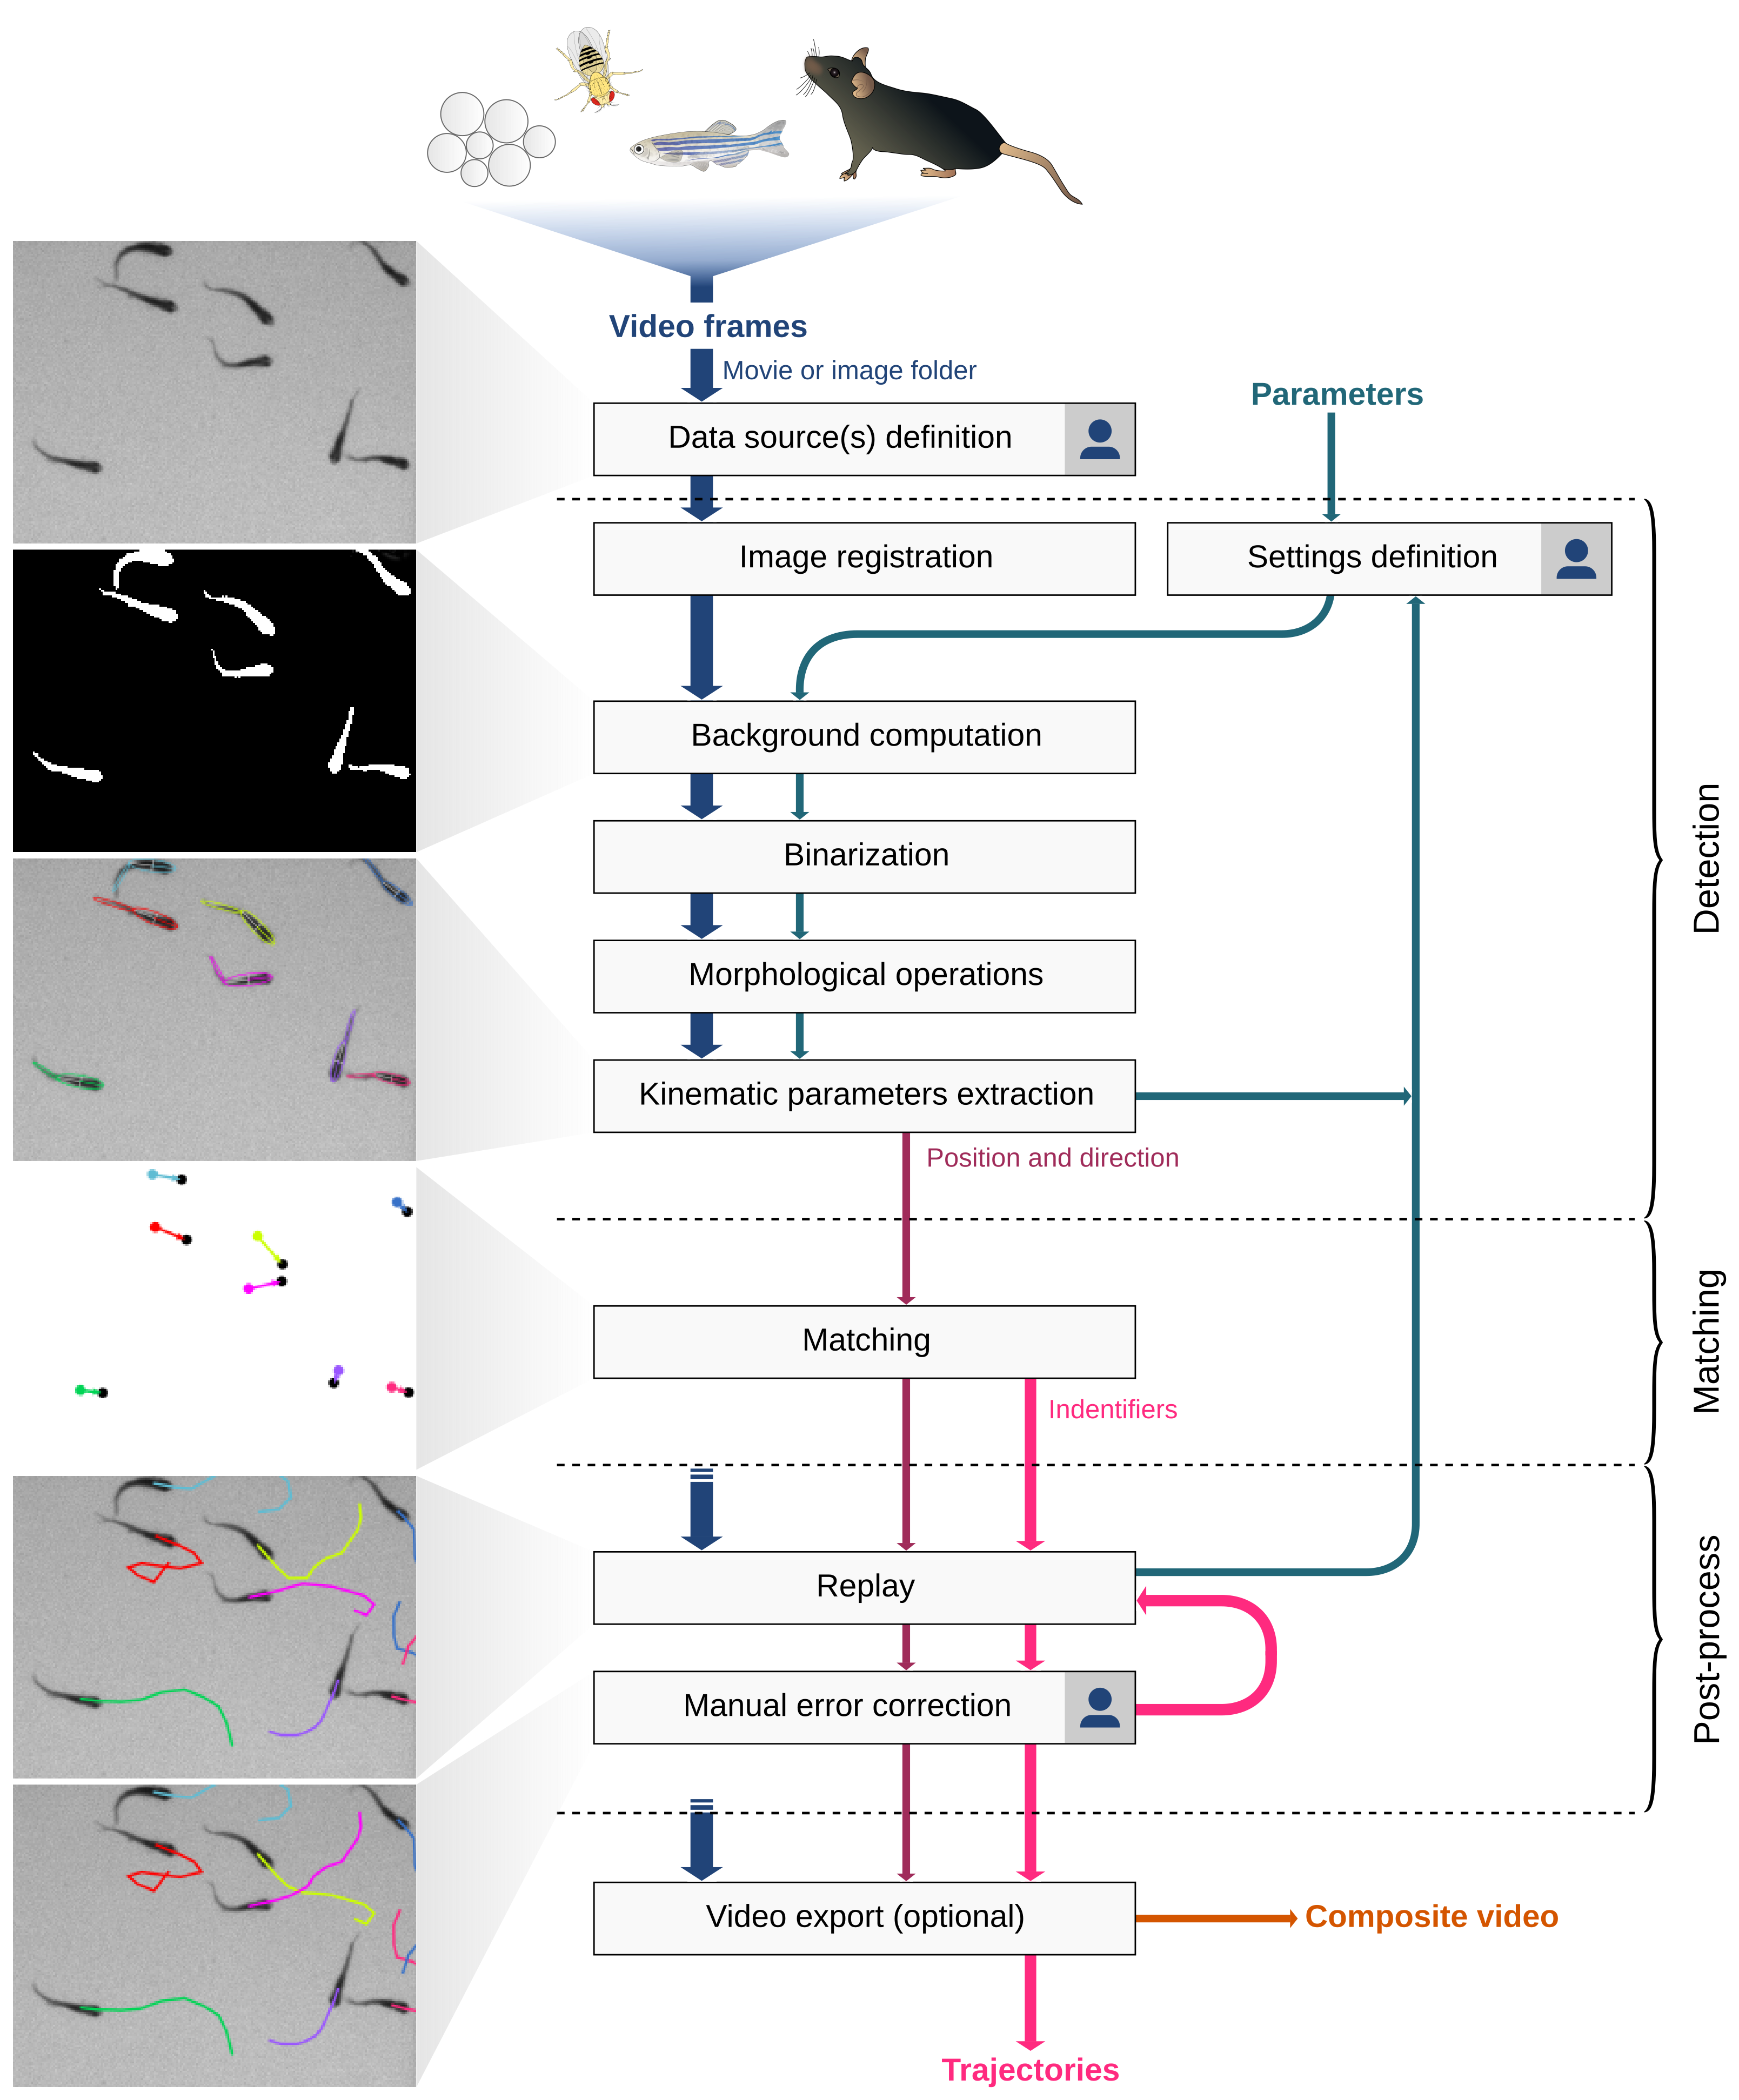
\includegraphics[width=0.75\textwidth]{part_1/assets/Figure_1.png}
    \caption{{\bf FastTrack workflow chart.} The workflow divides into three mains parts: detection, matching, and post-processing. A \faUser indicates the few steps that require user input. Sample dataset: $ZFJ\_001$.}
    \label{part_1:fig_1}
    \end{figure}

    \subsection{Detection}
    The purpose of the detection step is to extract each object's kinematic parameters, which will be used later in the association step. FastTrack includes a collection of image analysis filters that allow the user to optimize object detection without external software.
    \paragraph{Background Calculation}
    Each analysis starts by calculating a background image. If the user already has a previously saved background image, he can directly open it in the software. Otherwise, three calculation methods are possible:
    \begin{itemize}
        \item Projection of maximum intensity.
        \item Projection of minimum intensity.
        \item Projection of the average intensity.
    \end{itemize}
    All three methods are based on the same principle. The user chooses $n$ images in the sequence. The software will make a projection of the stack along the time component, either the maximum, minimum or average of each pixel. In practice, the maximum (resp. minimum) will be projected if the objects are darker (resp. lighter) than the background so that the objects disappear and thus obtain the background. The user can make the registration of each image before the projection in order to correct a possible camera movement.

    \paragraph{Registration}
    The user can choose to register the images. Three methods are proposed in the software. Each method is implemented in a pyramidal way, i.e., the registration is first carried out on a degraded image to roughly correct the displacement. The correction is then refined by increasing the image quality until the original quality is reached. This speeds up the process, as registration is often a relatively time-consuming process.

    The first method proposed is phase correlation. It allows correcting the translational movements between two images using the Fourier theorem in the frequency domain. This method is swift but remains limited to small translational movements only.

    The second proposed method is the Enhanced Correlation Coefficient (ECC) \cite{evangelidis2008parametric} method. In FastTrack, it is restricted to correcting translational and rotational movements only. It consists of using the correlation coefficient as a measure to find the best transformation between two images. This method's advantage is that it is relatively fast since this non-linear optimization problem can be solved linearly. It is efficient for noisy images and having photometric distortions.

    The third method is a method based on the identification of key points. It allows for correcting movements and deformations (homography). The key points (about 500) are automatically determined on two images thanks to the ORB algorithm \cite{rublee2011orb}. These points are then associated two by two using the hamming distance. The RANSAC algorithm \cite{bolles1981ransac} is used to find the best transformation between the two images. This method, more precise, requires a sufficient image quality to be able to discern key points.

    \begin{figure}[h!]
    \centering
    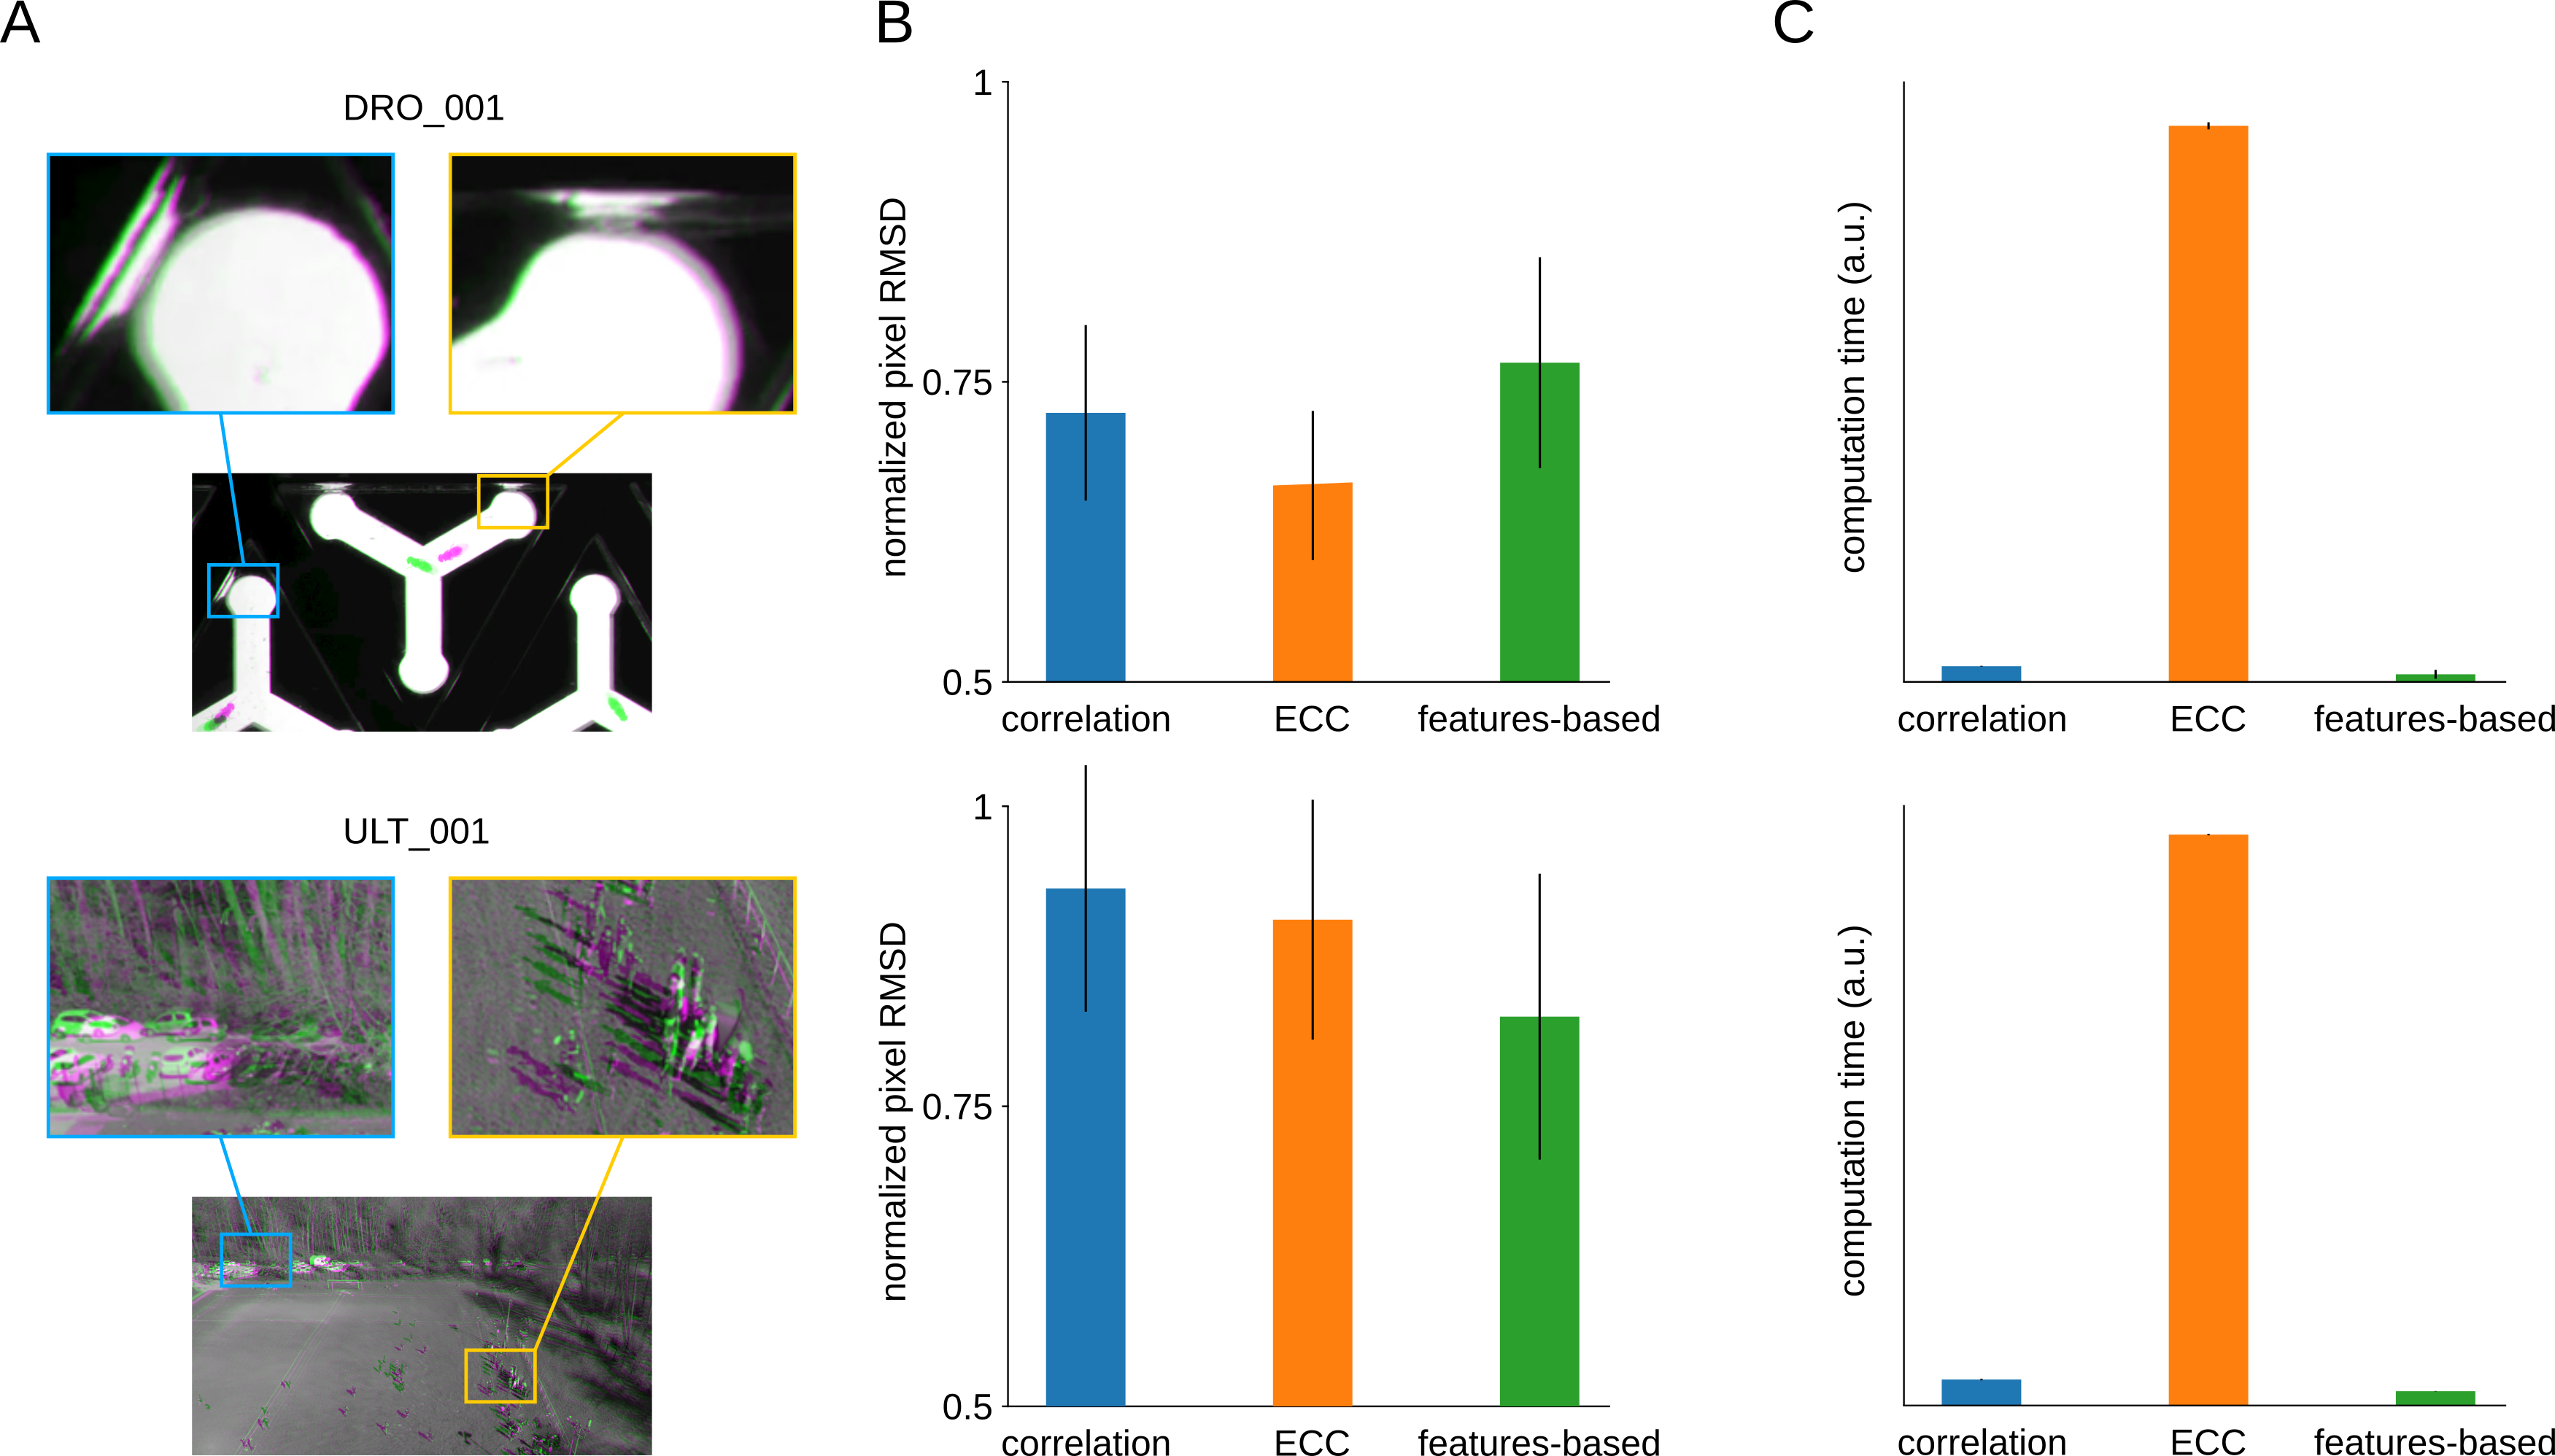
\includegraphics[width=1\textwidth]{part_1/assets/Figure_2.png}
    \caption{{\bf Image registration.} Two recordings with severe drift are used for the benchmarking (top: $DRO\_001$, bottom: $ULT\_001$).
        (\textbf{A}) Comparison of a frame (magenta) with the first frame (green) and magnification of details in the scene.
        (\textbf{B}) The root mean square deviation (RMSD) of pixel intensities after registration onto the first image, averaged over all time frames and normalized by the RMSD without registration, for the three registration methods. Error bars: standard deviation across time frames.
        (\textbf{C}) The relative average computation time of the three registration methods, normalized by the total number of pixels in the movie (arbitrary units). Error bars: standard deviation across time frames.}
    \label{part_1:fig_2}
    \end{figure}

    Figure~\ref{part_1:fig_2} provides a rough comparison of the performance of the three methods. Using two recordings of the dataset, we benchmarked both the accuracy – with the root mean squared difference (RMSD) of pixel intensities between the reference and the corrected image – and the relative computation time. Choosing the right method to obtain the best accuracy depends on each movie’s characteristics. However, one can use the rule of thumb that if the objects to track occupy a large fraction of the total area, the best accuracy is more likely to be obtained by using ECC and using the features-based method otherwise. However, as shown in Figure~\ref{part_1:fig_2}-C, the ECC method is generally slower by an order of magnitude. Hence, we recommend using the features-based method in the general case and long movies.

    \paragraph{Binarization}
    Each image is then binarized by subtracting the background image and defining a threshold value. In the interactive mode, the user can see the impact of the parameters on the image, which makes it easier to adjust the binarization threshold. The software also detects if the background is darker (resp. lighter) than the objects allowing to have at the end of this operation a binary image where the pixels belonging to the object are equal to 1, and the pixels belonging to the background are equal to 0.

    \paragraph{Morphological operation}
    A set of morphological operations (dilation, erosion, opening, etc.) can be performed on the binary image to improve detection and eliminate possible artifacts. Different shapes and sizes of kernels are available.

    \paragraph{ROI}
    The user can select a region of interest and exclude the rest of the image from the analysis. This speeds up the analysis process and avoids the detection of interfering objects. In interactive mode, this ROI can be drawn directly on the image.

    \paragraph{Sorting}
    To exclude objects that are too small (e.g., noise) or too large ( e.g., two objects overlapping each other), the user must select two characteristic sizes. The objects are colored either red or green in the interactive mode depending on whether their size belongs to the selected range.

    \paragraph{Extracting kinematic parameters}
    Based on the binary images, the software will detect the contour of each object. An essential step in any tracking procedure is the extraction of the parameters used in the association step. It is generally with the choice of these quantities that the tracking algorithms can differ to be more specialized for a given type of object. In FastTrack, the parameters extracted are the center of mass, the orientation, the area, and the object's perimeter. These quantities are quickly calculated and general enough to adapt to a wide variety of objects.

    To do this, FastTrack calculates the object's equivalent ellipse from the second-order moments of the binary image. This procedure is accelerated by directly using the contour thanks to Green's formula \cite{Riemann B.}. The object's orientation is given by the ellipse's major axis and is defined in the interval $[0;\pi[$. The direction in the interval $[0; 2\pi[ $ is determined by projecting each object's pixel on the major axis of the equivalent ellipse, and calculating the skewness of the distribution of distances of these projected points to the center of mass. The skewness sign is a robust indicator of the object's asymmetry along its principal axis.
    For deformable objects, the previously calculated direction may be different from the direction of motion. For example, in the case of zebrafish, it bends its body periodically to move. Only the head is directed at the motion. This is why the object is decomposed into two equivalent ellipses. The user can then choose which ellipse best represents the direction of the movement.

    \begin{figure}[h!]
    \centering
    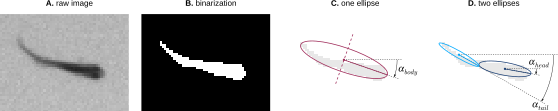
\includegraphics[width=1\textwidth]{part_1/assets/Figure_ellipse.png}
    \caption{\textbf{Detection} Details of the detection phase for one object of the movie $ZFJ\_001$.
        (\textbf{A}) raw image.
        (\textbf{B}) binarized image obtained by subtraction the background image and applied a threshold.
        (\textbf{C}) equivalent ellipse of the object.
        (\textbf{D}) two equivalent ellipses, useful for a deformable object.}
    \label{part_1:fig_2}
    \end{figure}

    \subsection{Association}
    The purpose of the association step is to keep the objects' identity from one image to another. To do so, FastTrack uses a method derived from \cite{qian2016effective}, which takes advantage of the fact that each object's position, area, perimeter, and direction changes very little from one image to another.

    For each pair of objects $(i,j)$ belonging to two successive images, two costs are calculated.
    The hard cost as follows:
    $$
    \left\{
        \begin{array}{ll}
            h_{i,j} = 1 & \mbox{if } r_{i,j} < h_{d} \\
            h_{i,j} = \inf & \mbox{else }
        \end{array}
    \right.
    $$
    \noindent with $r_{i,j}$ the distance between objects i and j, $h_{d}$ a threshold representing the maximum travel distance allowed between two successive images. The hard cost allows discarding obvious impossible assignments to speed-up the computation. It is essential with a non-constant number of objects because it allows new objects entering the field of view to be assigned with new identities.

    The soft cost is defined as follows:
    $$
    c_{i,j} = \frac{r_{i,j}}{s_d} + \frac{\delta\alpha_{i,j}}{s_{\alpha}} + \frac{a_{i,j}}{s_a} + \frac{p_{i,j}}{s_p}
    $$
    \noindent where $\delta\alpha_{i,j}$ is the angular difference, $\delta a_{i,j}$ the area difference and $\delta p_{i,j}$ perimeter difference between objects i and j. To compare these quantities expressed in different dimensions and magnitudes, we need to normalize them. We define the soft normalization coefficients: $s_{d}$, $s_{a}$, $s_{p}$ and $s_{\alpha}$. These coefficients represent the typical value of the parameter that they normalize.
    We can construct the cost matrix:
    $$
    C_{i,j} = \left\{
        \begin{array}{ll}
            c_{i,j} & \mbox{if} r_{i,j} < h_{d} \\
            \inf & \mbox{else}
        \end{array}
    \right.
    $$
    This cost matrix is, in general, rectangular because the number of objects can vary from one image to the following. A memory parameter can be selected to assign a new identity to an object that disappears on more than the selected number of images. In this case, we remove the row corresponding to this object from the cost matrix.
    We want then to find the best possible association. This problem is called the rectangular assignment problem and can be solved exactly by using the Hungarian algorithm see Annexe~\ref{appendix_hungarian}. FastTrack uses the Kuhn-Munkres implementation in C++ to solve it.

    \subsection{Automatic tracking parameters}
    Finding the optimal tracking parameters is necessary to have a tracking accuracy as good as possible. FastTrack can automatically determine a neutral set of soft normalization factors $s_r$, $s_\alpha$, $s_A$, and $s_p$ to help the user. These factors allow comparing terms of very different nature and amplitude into a single cost function. The set of parameters automatically found by FastTrack will give each term the same weight inside the cost function. Therefore, the user must perform parameters' fine-tuning, with some system insight, to get the best set of parameters possible.

    It is intuitive to use the standard deviation of the increments of each kinematic parameter. However, some trajectories are needed to estimate the standard deviations. We set up an iterative, rapidly-converging algorithm to perform this talk.

    Let us use $ZFJ\_001$, a slightly oversampled movie, with many occlusions and objects of different sizes to illustrate the algorithm's details. For simplicity, let us use only the position, angle, and area as kinematic parameters. There is no gain to expect by adding the perimeter parameter because objects' shapes are very similar. The Figure~\ref{part_1:fig_5}-A. shows a snapshot of this movie.

    To evaluate the distributions of $dr$, $d\alpha$, and $dA$, we start by tracking the movie setting the hard parameters and random soft parameters. The resulting distributions are shown in Figure~\ref{part_1:fig_5}-C to E. For kinematic parameters whose differential values can be positive or negative, the distribution is fitted by a Gaussian function, and the soft parameter is set to the standard deviation. For instance, with the angular difference $d\alpha$ the fit reads:

    \begin{equation}
    f(d\alpha) = \frac{1}{s_\alpha\sqrt{2 \pi}} \; e^{-\frac{d\alpha^2}{2 s_\alpha^2}}
    \label{eq:fit_Gaussian}
    \end{equation}

    \noindent and $s_\alpha$ (orange bar in Figure~\ref{part_1:fig_5}-D) is stored as the soft parameter to use during the next iteration.
    The computation of the soft parameter for the displacement $s_r$ is different since distances can only be positive. Assuming that the displacements along the $x$ and $y$ axes follow two independent Gaussian processes, the resulting displacement follows a $\chi$ distribution with $2$ degrees of freedom, and the fit reads (see Annexe~\ref{} for de detailed derivation):

    \begin{equation}
        f(x)
        \label{eq:fit_chi}
    \end{equation}

    \noindent where $s_r$ (orange bar in Figure~\ref{part_1:fig_5}-C) is stored as the soft parameter to use for the next iteration.

    Once all soft tracking parameters have been derived from the distributions, the software recomputes new trajectories with these updated parameters. This iterative process, depicted in Figure~\ref{part_1:fig_5}-B, is run until the tracking parameters converge. In practice, the convergence is very fast, regardless of the initial position in the parameters space. We drew $100$ sets of seed parameters from uniform distributions spanning large intervals, and convergence has been attained in very few iterations for all parameters Figure ~\ref{part_1:fig_5}-F.

    FastTrack's implements this algorithm by taking the kinematic quantities' sample standard deviation for a subset of 200 images in the movie to increase speed and efficiency. The convergence criterion implemented is that soft parameters should vary less than $10^{-3}$.

    To characterized the resulting tracking, we computed the number of swaps with respect to the ground-truth:

    \begin{equation}
    P_{swap} = \frac{N_{swap}}{N_{obj} - n_{ap}}
    \label{eq:Pswap}
    \end{equation}

    \noindent with $N_{swap}$ being the total number of swaps, $N_{obj}$ the total number of objects on all frames and $n_{ap}$ the number of times a new object appears. If the number of objects is constant and noted $n$, then $n_{ap} = n$ and $N_{obj} = nT$, with $T$ the number of frames in the recording, such that $P_{swap}$ can be simpliefied:

    \begin{equation}
    P_{swap} = \frac{N_{swap}}{n(T-1)}
    \label{eq:Pswap_constant}
    \end{equation}

    $P_{swap}$ converges very fast to a value that is nearly-optimal. For $77\%$ of the parameter sets $P_{swap}$ is decreased or remain equal, with an average drop of $0.0119$ ($155$\% of the converged value), while for 23\% of the parameter sets $P_{swap}$ is increased with an average rise of $0.0011$ ($14$\% of the converged value). Thus, the expected difference is $-0.0090$ ($116$\% of the converged value) for this movie. Therefore, the automatic parameters are an excellent starting point in the general case. The user can fine-tune the weights given to the kinetic parameters to consider the specificities of each movie.

    We computed the converged soft parameters $\hat{s}_r$, $\hat{s}_\alpha$ and $\hat{s}_A$ for several sampling rates of $\tau>1$ (Figure~\ref{part_1:fig_5}-H to J). We used these parameters to track the $ZFJ\_001$ movie at different $\tau$ and compute $P_{swap}$. A comparison between $P_{swap}$ and $P_{inc}$ as a function of $\tau$ is shown in Figure~\ref{part_1:fig_5}-K. This comparison illustrates that $P_{swap}$ is a noisier measurement of a movie's trackability than $P_{inc}$ and confirms that the iterative algorithm produces trajectories with a number of errors that is close to the statistical limit.

    \begin{figure}[h!]
    \centering
    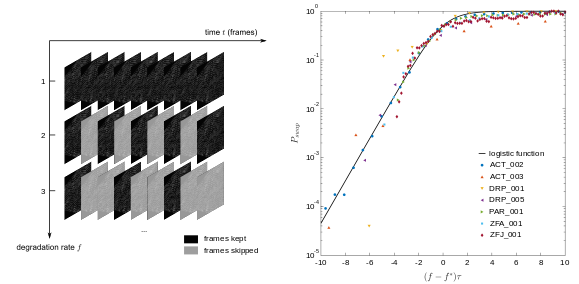
\includegraphics[width=1\textwidth]{part_1/assets/Figure_5.png}
    \caption{{\bf Automatic tracking parameters.}
        (\textbf{A}) Snapshot and blow-up of $ZFJ\_001$ movie, with definition of $\vec{dr}$ and $d\alpha$
        (\textbf{B}) Scheme of the algorithm determining the tracking parameters automatically.
        (\textbf{C-E}) Distribution of displacements $dr$ (in pixels), angular differences $d\alpha$ (in radians) and area differences $dA$ (in pixels) when the default parameters of the software are used on $ZFJ\_001$, for $\tau=1$ (black). The corresponding $\chi$ and Gaussian fits are displayed in red. Orange bars: resulting soft parameters.
        (\textbf{F}) Evolution of $s_r$, $s_\alpha$ and $s_A$ with algorithm iterations for $ZFJ\_001$. Left: iterations 1 and 2; right: iterations 2 and 3. A hundred runs with random initial values are shown. The run with the software default parameters is highlighted in red.
        (\textbf{G}) Evolution of $P_{swap}$ with algorithm iterations, same runs.
        (\textbf{H-J}) Evolution of the converged parameters $\hat{s}_r$, $\hat{s}_\alpha$ and $\hat{s}_A$ as a function of the timescale $\tau$ for $ZFJ\_001$.
        (\textbf{K}) Comparison between $P_{swap}$ (blue crosses) obtained with the converged parameters and $P_{inc}$ (red dots) for $ZFJ\_001$. The solid black line is the logistic fit of $P_{inc}$.}
    \label{part_1:fig_5}
    \end{figure}

    \subsection{Manual correction}
    FastTrack integrates a manual tracking correction tool. Once the analysis is completed, the result can be displayed in an ergonomic interface created solely for this purpose. The user can replay the film by superimposing the results of the analysis on the original movie. The user can interactively see each object's parameters. More importantly, the user can also correct tracking errors by deleting objects or exchanging objects' identity.
    This interface is designed with ergonomics and performance in mind. Keyboard shortcuts and an on-the-fly selection of objects by clicking on the video allow the user to check and correct the analyses quickly. It is also possible to record a film with the tracking results overlay superimposed.
    This manual correction interface makes it possible to shift the workload from the traditional pre-processing of data to the tracking result's post-processing. In general, tracking software will reduce user inputs and improve tracking by using the raw images' pre-processing and the conception of system-specific tracking algorithms. With FastTrack, the pre-processing step is reduced to the minimum to remain general and be applied to a wide variety of systems. To compensate for this, FastTrack provides a correction tool. In the following chapter, we will see that this method can save the user much time because the correction time is in general lower than the conception and computational time of system-specific tracking algorithms.

    \subsection{Analysis}
    A question that comes back a lot from users' feedbacks is what to do after the tracking. FastTrack only takes care of the tracking, and statistical data analysis is not implemented in the software. After the tracking, the software generates several files containing the results and the tracking parameters. The result file is named tracking.txt, and it contains the raw data of the analysis with one image and one object per line. This format is compatible with the most used analysis software (R, Python, Julia, spreadsheet). Examples in Python and Julia are available in the documentation to get started.

	\section{Deployment}
    \subsection{CI/CD}
    \label{part_1:cicd}

    \begin{figure}[h!]
    \centering
    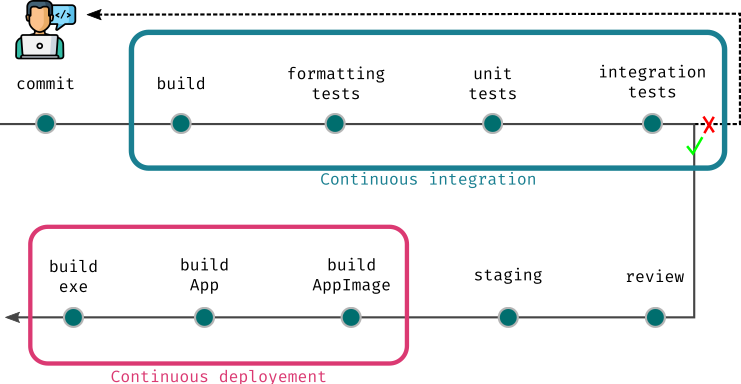
\includegraphics[width=1\textwidth]{part_1/assets/Figure_cicd.png}
    \caption{{\bf FastTrack CI/CD workflow.} The CI/CD workflow is divided into two parts: the CI tasks (blue rectangle) and the CD tasks (red rectangle). The CI must be performed successfully in order to integrate the changes into the project.}
    \label{part_1:fig_cicd}
    \end{figure}

    The deployment is one part that should not be overlooked in software design, and two aspects are crucial to consider. From the user's point of view, the software must be easy to install on supported platforms and with fewer bugs as possible. From the maintainer's perspective, the deployment part must be easily achievable and reproducible so that patches and new functionalities can be quickly integrated. From the developer's perspective, the source code's consistency and correctness have to be tested at each change to avoid introducing bugs and facilitate collaboration between developers.  With this in mind, FastTrack follows the CI/CD philosophy \cite{shahin2017continuous}\cite{wikstrom2019benefits} taking advantage of the new GitHub Actions system.

    Continuous Integration (CI) is a set of practices designed to integrate changes quickly into the project in an automated manner. It is coupled with the automation of unit testing. FastTrack takes advantage of GitHub's CI/CD system called Actions. With each new (commit\footnote{Action to send the list of changes made in the version management system}) or new (pull-request \footnote{Action to request the addition of changes to the project}), a series of tests is automatically triggered. These tests will check the proper functioning of the tracking algorithm and the formatting of the source code. Only the changes that pass the tests can be integrated into the project, which guarantees the reproducibility of the analyses and the source code and documentation consistency.

    Continuous Delivery (CD) automates the delivery of the software in its final form. It allows changes to be quickly integrated into the software without manually doing it for each supported platform. In the case of FastTrack, the CD is implemented using GitHub Actions, and a new version of the software is compiled for Linux, macOS, and Windows with each new commit that is integrated into the main branch. Stable versions of the software are compiled at regular intervals of the development. This system is a significant time-saver for multi-platforms software like FastTrack. It allows the user always to have the latest patches and features available. The developers can collaborate easily on the project, and the maintainer can quickly produce binaries for the supported platforms.

    FastTrack natively supports the three most commonly used platforms: Linux systems with an AppImage that supports all distributions, Windows with an installer, MacOS with an App. The latest stable version can be downloaded from the website \url{http://www.fasttrack.sh}, the nightly build version from \url{https://github.com/bgallois/FastTrack/releases}. The procedure to compile the software itself is available in the developer's documentation.

    \subsection{Documentation}
    FastTrack offers extensive documentation that covers the installation and utilization of the software. Developer documentation with a documented API and a compilation guide is also available for users wanting to integrate FastTrack in their software or workflow.

    \paragraph{User} User documentation is available at \url{https://www.fasttrack.sh/UserManual/docs/intro.html}. This documentation is generated from the project, and users can contribute to it at https://github.com/bgallois/FastTrack/. It contains all the information needed to use the software and instructional videos to help the user get started with the software.
    \paragraph{Developer} Developer documentation is available at \url{https://www.fasttrack.sh/API/index.html}. It is automatically generated by the Doxygen software from the documentation in the FastTrack source code. It contains all the information necessary for developers who want to modify or contribute to FastTrack.


\chapter{Movies dataset}
    To demonstrate that FastTrack can analyze movies from various systems, we have compiled a database of movies named $TD^2$. This database can be downloaded at \url{https://data.ljp.upmc.fr/datasets/TD2/}. The films either come from data already published in the literature or provided to us by the authors themselves. All the movies are under a CC-BY-NC-SA license. Each movie is identified by a 3-letter code defining the system (e.g., ACT: active matter, ZFA: zebrafish adult...) and three digits to index films from an identical system. $TD^2$ currently regroups 41 films, including different types of objects of very different nature and size
    \begin{itemize}
    \item 7 species of animals from fish to flies,
    \item cells,
    \item active particles,
    \item microfluidic drops,
    \item macroscopic objects such as ultimate players or cars.
    \end{itemize}
    A video giving a quick overview of all the systems used is available at \url{http://www.fasttrack.sh/images/illustrations/mockups/trackingExample.webm}.

    Another essential aspect to consider is the number of objects per film and their possible appearances, disappearances, and overlaps. In 22 films out of 41, the number of objects is variable, and objects come and go out of the camera field during recording. In 19 films out of 41, objects may overlap, creating an occlusion phenomenon that the software has to manage to preserve the identity of the objects.

	\begin{figure}[ht]
    \centering
    \includegraphics[width=1\textwidth]{part_1/assets/Figure_td2.png}    
    \caption{{\bf $TD^2$} Thumbnail of the $TD^2$ dataset.}
    \label{part_1:fig_5}
    \end{figure}

    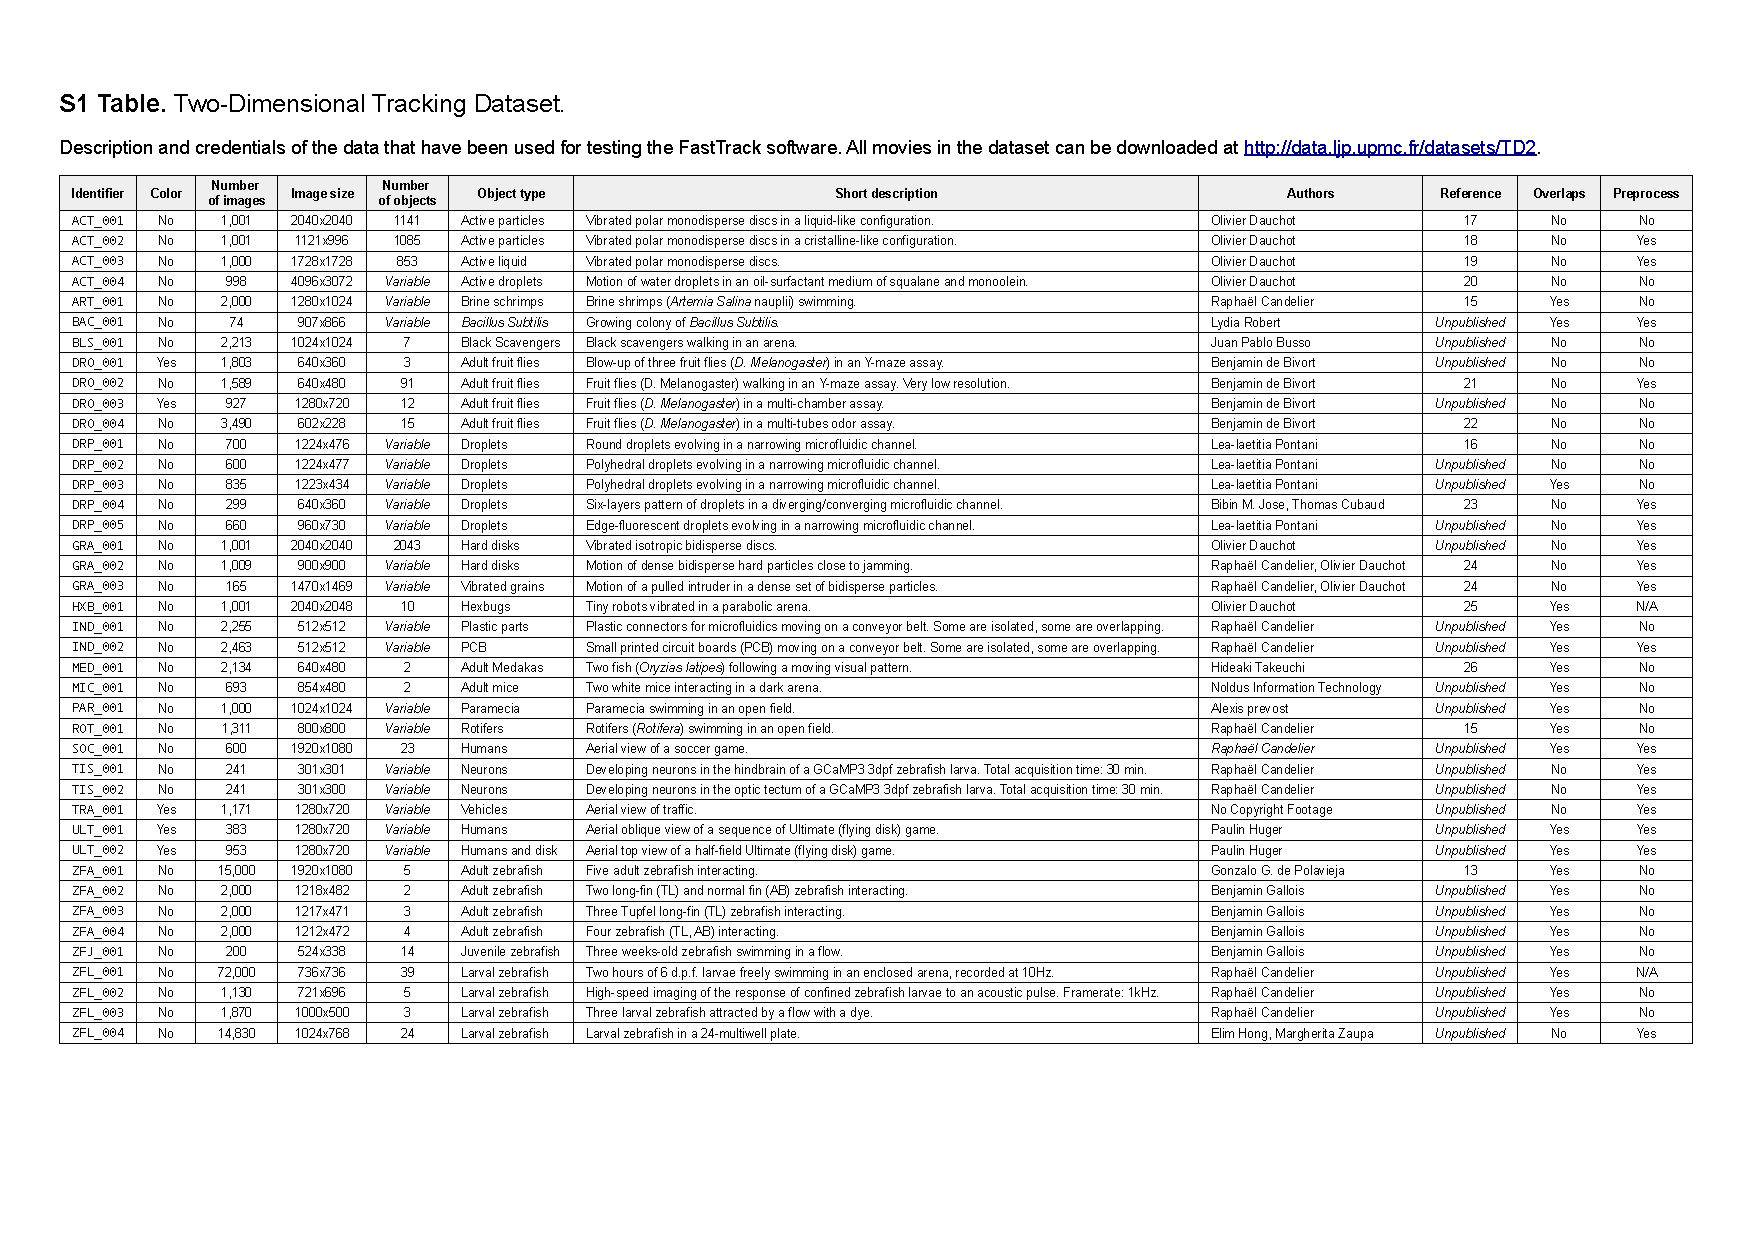
\includepdf[landscape=true]{part_1/assets/Table_td.pdf}


\chapter{Results}

    \section{Performance}
    To assess FastTrack's performance, we ran a benchmark comparing FastTrack, Idtracker.ai, and ToxTrac. These software have substantial intrinsic limitations compared to FastTrack. Both require an acceptable framerate and image quality, with sufficient contrast and number of pixels per object and a constant number of objects in the movie that must be defined before the tracking. The benchmark was performed on a dataset consisting of a selection of videos provided with each software, and some movies from the $TD^2$ dataset that meet the three software requirements. $idtrackeraivideoexample$ and $100Zebra$ are available on the idtracker.ai website \url{https://idtrackerai.readthedocs.io/en/latest/data.html}. Guppy2, Waterlouse5, and Wingedant on the ToxTrac SourceForge\url{https://sourceforge.net/projects/toxtrac/files/ScientificReports/}. Movies provided in image sequence format were converted losslessly to a video format using FFmpeg since idtracker.ai and ToxTrac could not directly process image sequences. $DRO\_002$ and $ACT\_002$ were preprocessed with a custom script to detect the objects before performing the tracking. Also, only the first 100 images of $DRO\_002$ were used to reduce the computing time.

    The benchmark between idtracker.ai and FastTrack was performed on a workstation with an Intel i7-6900K (16 cores), 4.0 GHz CPU, an NVIDIA GeForce GTX 1060 with 6GB of RAM GPU, 32GB of RAM, and an NVMe SSD of 250GB running Arch Linux. The parameters were set by trials and errors inside the graphical user interface of the two software. The tracking duration was recorded using a script calling the software command-line interface. The average tracking duration and the standard deviation were computed over five runs except for $DRO\_002$  (2 runs) and $ACT\_002$ (1 run) due to the very long processing time. Idtracker.ai was evaluated with and without GPU capability except for $100Zebra$, $DRO\_002$, and $ACT\_002$ due to the very long processing time.

    The benchmark between ToxTrac and FastTrack was performed on a computer with an Intel i7-8565U (4 Cores), 1.99 GHz CPU, 16 GB of RAM, and an NVMe SSD of 1 TB running Windows 10. The parameters were set by trials and errors in the graphical user interface. The average tracking duration and the standard deviation were computed over five runs using each software's built-in timer feature. The accuracy was evaluated manually using the built-in review feature implemented in each software. The number of swaps and the number of non-detected objects were counted in each movie, and occlusion events were ignored in this counting.

	\begin{figure}[h!]
    \centering
    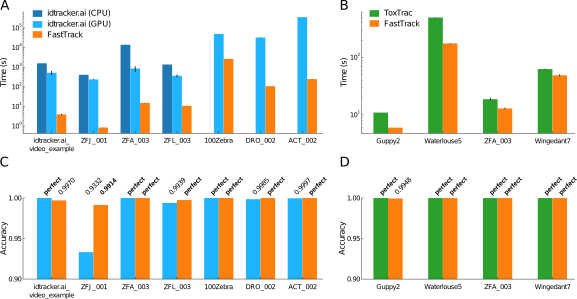
\includegraphics[width=\textwidth]{part_1/assets/Figure_benchmark.png}
    \caption{{\bf Benchmark of FastTrack, idtracker.ai, and ToxTrac.}
        (\textbf{A-B}) Comparison of the computation time for the tracking of various movies with the same workstation. Whenever possible, CPU and GPU variants of idtracker.ai have been run. Only the first 100 images of $DRO\_002$ have been used.
        (\textbf{C-D}) Accuracies of the resulting trackings. "perfect" means an accuracy of exactly $1$. The trajectories computed by the CPU and GPU variants of idtracker.ai being rigorously similar, we only show the GPU results. For $100Zebra$, the accuracy was computed by taking into account only the first 200 images.}
    \label{part_1:fig_benchmark}
    \end{figure}

    The accuracy was computed as follows:
    $$ A=\frac{n_{obj}n_{img} - (2N_{swap} + N_{undetected})}{n_{obj}n_{img}}$$
    with $N_{swap}$ the number of swaps, $N_{undetected}$ the number of non-detected objects, $n_{obj}$ the number of objects, and $n_{img}$ the number of images.
    For $100Zebra$, the accuracy was computed only over the 200 first images. All the results are presented in Figure~\ref{part1_fig_benchmark}. As expected, FastTrack is several orders of magnitude faster than idtracker.ai and significantly faster than ToxTrac on all tested videos. That is mainly due to the method used, idtracker.ai using deep learning and ToxTrac cost optimization and the identity preservation algorithm.
    All software performed exceptionally well in terms of accuracy, except idtracker.ai on $ZFJ\_001$ probably because the resolution is not good enough.
    FastTrack's ergonomic post-processing interface can be used to reach a perfect tracking accuracy within a few more minutes. This built-in manual correction is not possible in ToxTrac and lacking ergonomy in Idtracker.ai.

    Altogether, FastTrack offers many assets compared to idtracker.ai and ToxTrac. The software is more versatile than its concurrents and more comfortable to use. The total time spent to track a movie is globally lower, in some cases by orders of magnitude, without sacrificing tracking accuracy.

	\section{Dataset classification}
    Analyzing movies from systems as different as those compiled in $TD^2$ is a real challenge. That is partly due to the recording conditions that can be very diverse and make object detection more complex. Two recurring difficulties can be discerned: variations in illumination (e.g., reflection in GRA\_001, shadows in SOC\_001) and overlapping objects (e.g., HXB\_001).

    In movies from the academic world, systems are often designed to limit or circumvent these two difficulties. It is common to find movies with a uniform and constant illumination. Also, quasi-2D confinement and a restricted number of objects in the camera field reduce the number of occlusions.

    In $TD^2$, 23 movies have an illumination good enough to be analyzed directly with FastTrack. The others had to undergo a specific individual pre-processing before being analyzed. Two movies with too many occlusions were discarded (HXB\_001 and ZFL\_001) because they could not be analyzed with FastTrack.
    The remaining 39 films could be analyzed with FastTrack without difficulty. The Kuhn-Munkres algorithm being of complexity $O(n^3)$ the calculation time is generally quite fast. Each film was then manually corrected using the built-in tool to get the ground-truth tracking.

    FastTrack is designed to keep the post-processing phase as light as possible. However, this phase workload varies greatly depending on the movie being analyzed. This workload can be quickly estimated for a given film by computing what we call the probability of incursion.

    First, we define the incursion as the exit of an object from its Voronoi cell (see Annexe~\ref{appendix_voronoi}), defined at a time $t$, after a travel time $\tau$. The number of incursions depends on
    \begin{itemize}
    \item the distribution of the displacements,
    \item the density of objects,
    \item the geometry of the Voronoï cell
    \item the degree of motion alignment of the displacements.
    \end{itemize}
    To consider the objects' density, we defined the reduced length $\rho=r\sqrt{d}$ where $r$ is the length and $d$ the density. We remark that typically $\rho=1$ is corresponding to the length between two objects, and $\rho=0.5$ is the length between an object and its Voronoï cell boundary.

    Assuming that the dynamic is uncorrelated with the geometric proprieties of the Voronoï cells, we can write the incursion probability as follows:
        $$P_{inc}=\int_{0}^{\inf} R(\rho)p_{inc}(\rho) \,d \rho$$
    where $R(\rho)$ the distribution of the reduced displacement at the timescale $\rho$, and $p_{inc}(\rho)$ the geometrical probability of incursion.

    $p_{inc}(\rho)$ depends only on the geometrical properties of the objects' arrangement. We can calculate $p_{inc}$ by taking a Voronoï cell and determining the proportion of the angles for which a displacement of $\rho$ implies an incursion in a neighboring Voronoi cell. In other words, see Figure~\ref{part_1:fig_pinc}, we take a circle of radius $\rho$ centered on the object and count $\Sigma$ the proportion of the circle that lies outside the Voronoï cell. That will give us $p(\rho)=\frac{\Sigma(\rho)}{2\pi}$ the geometric probability of incursion for one cell. Then, to take into account the diversity of size and shape of Voronoï cells, we average over all the cells of the movies $p_{inc}(\rho)=<p(\rho)>_{cells}$.

    Intuitively, we see that $p_{inc}$ goes from 0 when $\rho->\inf$, to 1 when $\rho>>1$. The precise shape of the geometric probability is sensitive to the density of objects, compact (e.g., ACT\_002), sparse (e.g., PAR\_001), and to the overall size of the system when walls restrict it (e.g., ZFA\_001).

	\begin{figure}[h!]
    \centering
    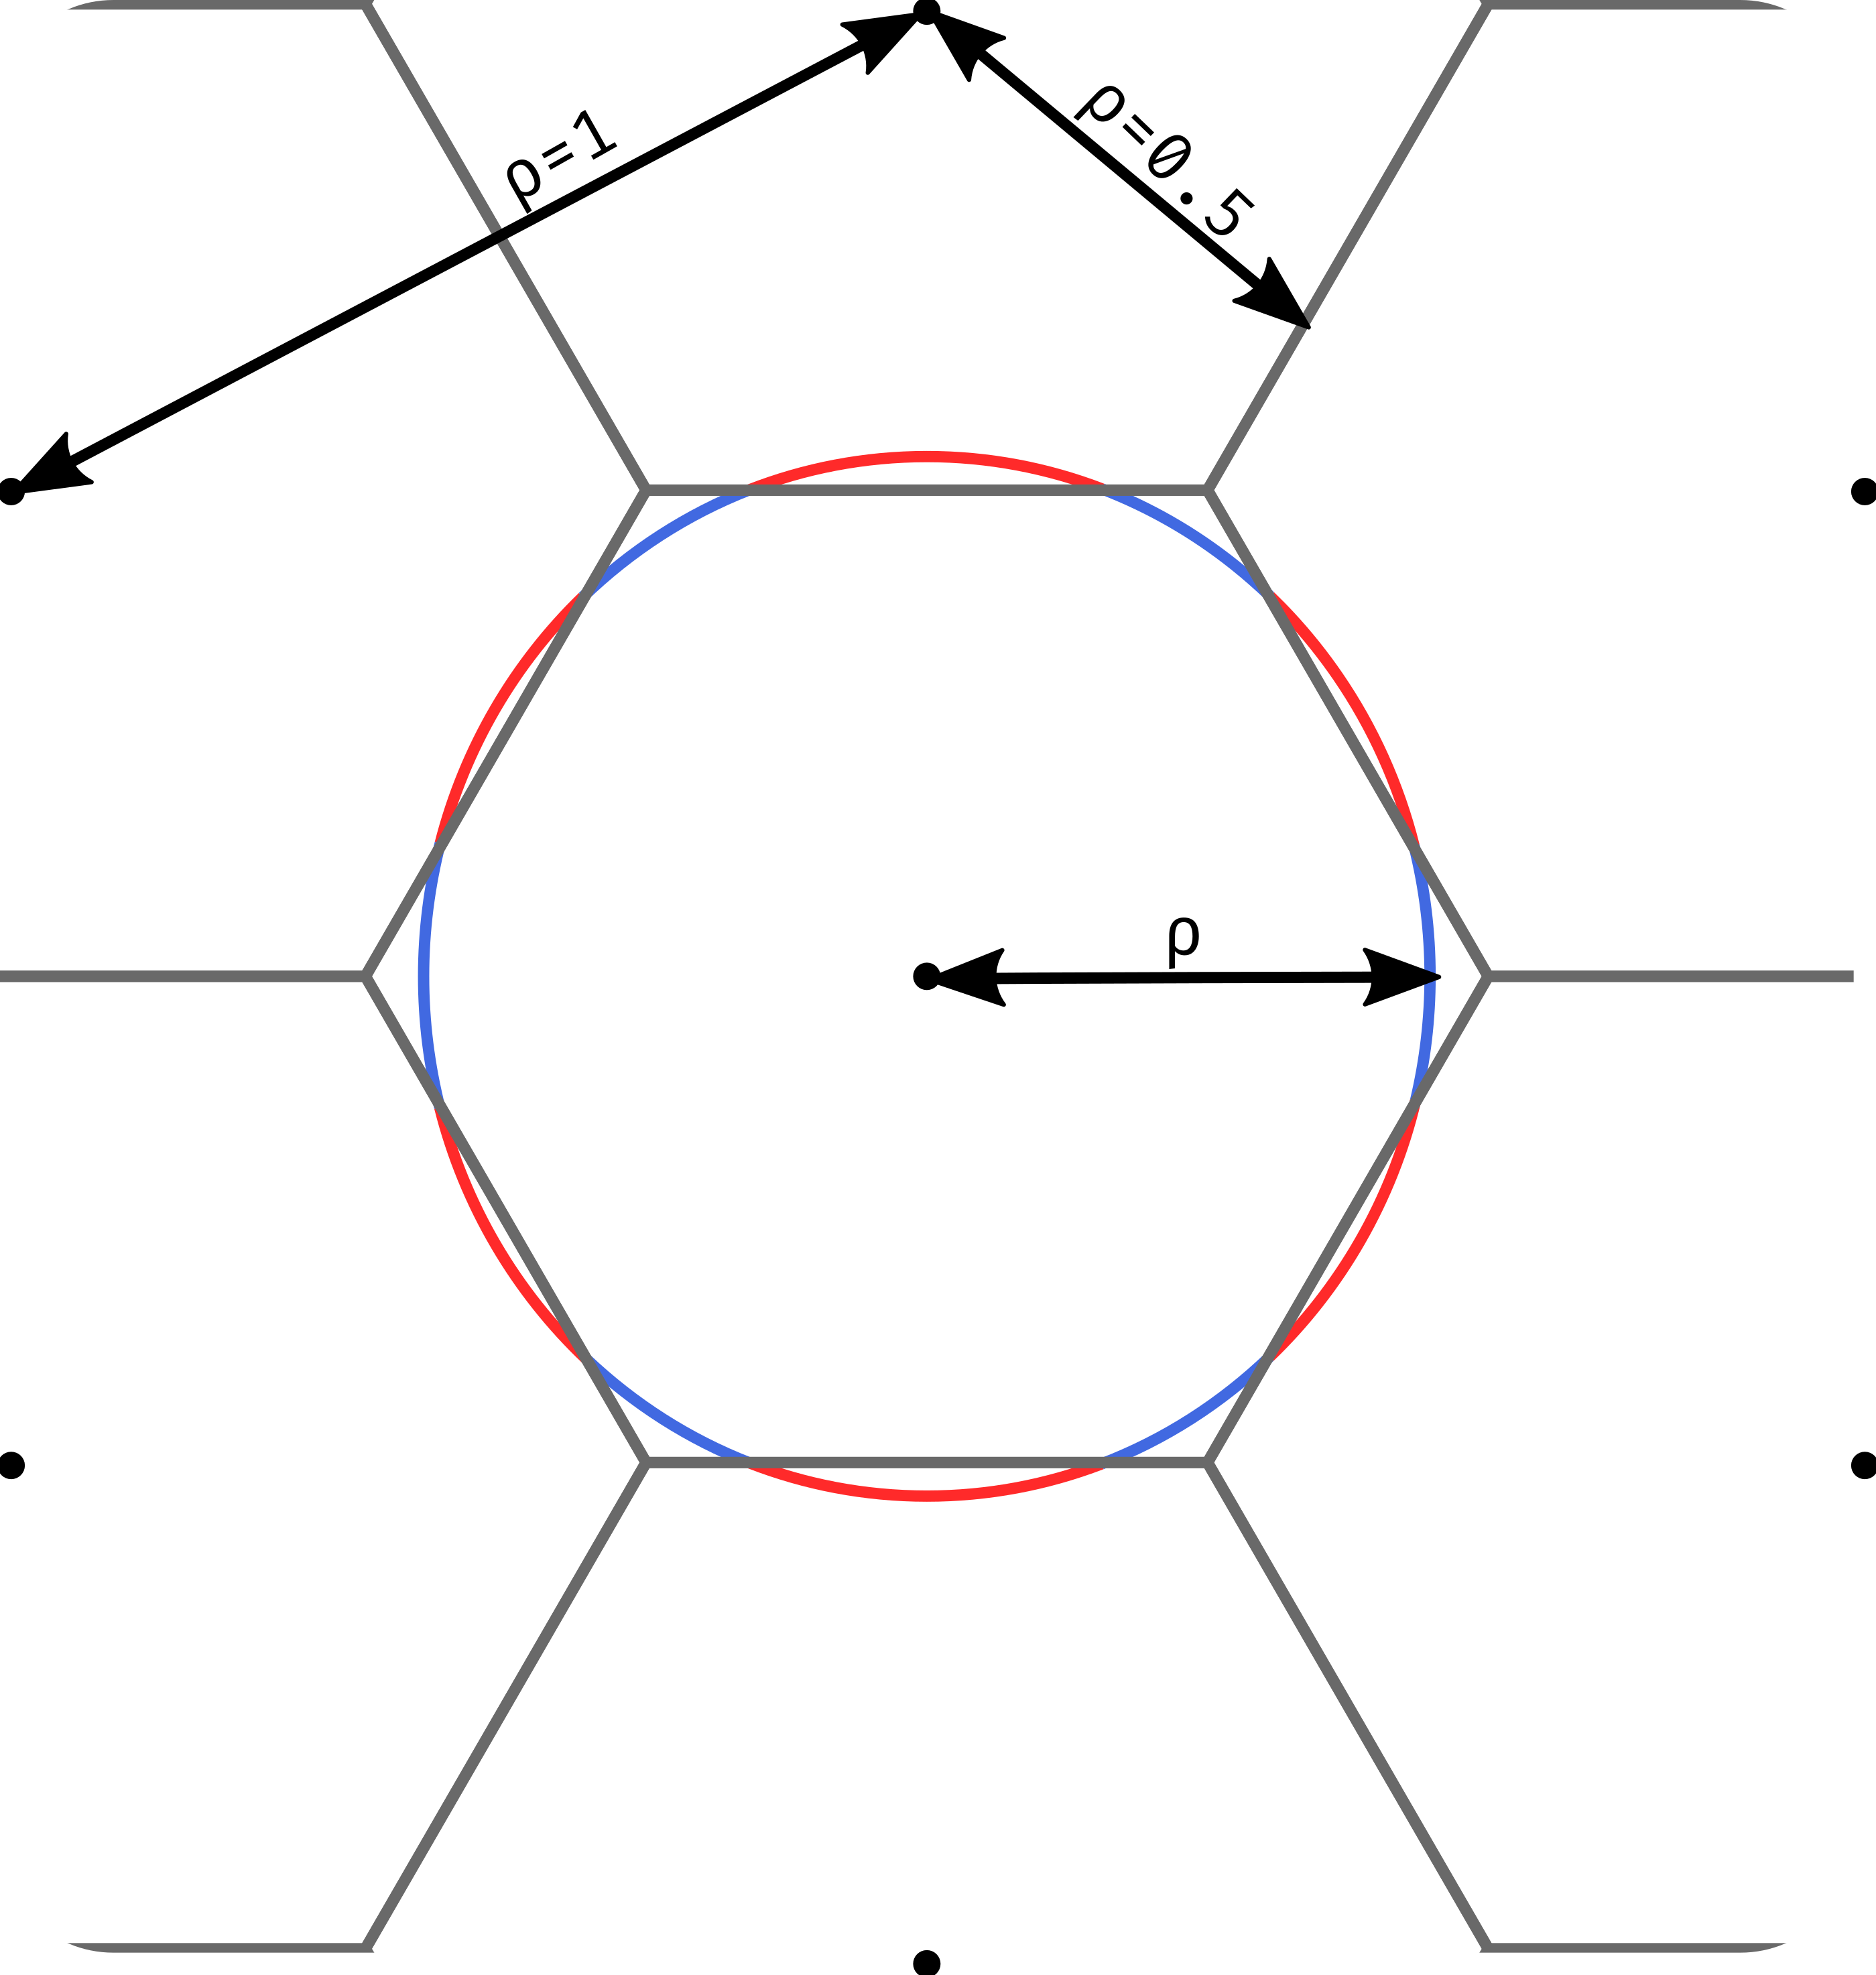
\includegraphics[width=0.5\textwidth]{part_1/assets/Figure_pinc.png}
    \caption{\textbf{Geometric probability of incursion:} Voronoï cells in black and objects black dots with typical $\rho$ length. Circle of radius $\rho$ with portions inside the Voronoï cell in blue and outside in red. The geometric probability for one cell is computed as $p(\rho)=\frac{\color{red}{\Sigma_{out}(\rho)}}{\color{red}{\Sigma_{out}(\rho)} \color{black}{+}\color{blue}{\Sigma_{in}(\rho)}} = \frac{\color{red}{\Sigma_{out}(\rho)}}{2\pi}$}
    \label{part_1:fig_pinc}
    \end{figure}

    The distribution $R(\rho)$ is shown in Figure~\ref{part_1:fig_3}.B for three timescales $\tau$. A graphical way of calculating $P_{inc}$ is to take the intersection of the areas under $R(\rho)$ and $p_{inc}(\rho)$. In the regime where $R(\rho)$ and $p_{inc}(\rho)$ are well-separated, the resulting value of $P_{inc}$ are low but highly sensitive to the number of swaps in the tracking. Indeed, the swaps create a bump in $R$  at values of $\rho$ close to one that can artificially increase $P_{inc}$ of several orders of magnitude. Unless the ground-truth trajectories are accessible, the single value of $P_{inc}$ at $\tau=1$ can not be used as a measure for a movie's trackability.

    A timescale-varying analysis will allow us to extract more robust quantifiers. As $p_{inc}(\rho)$ does not depend on $\tau$ and $R(\rho)$ is shifted to the high values of $\rho$ when $\tau$ increases, we can expect that $P_{inc}(\tau)$ has a sigmoid-like shape. We thus computed $P_{inc}$ for various $\tau$. If $\tau>1$ we take integer values (i.e. keep one frame every $\tau1$), and if $\tau<1$ we linearly interpolated the displacements (i.e. multiplied $\rho$ by $\tau$). We represented the results in Figure~\ref{part_1:fig_3}.C for the 39 movies that could be tracked in the dataset.

    Strikingly, all $P_{inc}$ followed a logistic curve when $\tau$ is log-scaled. Therefore we used a fit of the form:
    $$Pinc=\frac{L}{1 + e^{-k(log(\tau)-x_0)}}$$
    and, noting $\tau_0=e^{x_0}$, the fitting function can be rewritten as:
    $$P_{inc}=\frac{L}{1 + \frac{\tau_0}{\tau}^k}$$
    The fits are shown in Figure~\ref{part_1:fig_3}, and are valid for all the movies in the dataset. We can make all fitting curves collapse on a single master curve. We show in Figure~\ref{part_1:fig_3}.D that $\frac{P_{inc}}{L}$ plotted as a function of $klog(frac{\tau}{\tau_0})$ follows the standard logistic sigmoid function $$f(x) =\frac{1}{1+e^{-x}}$$.

    An exciting outcome of this approach is determining the framerate at which experiments should be recorded. It is indeed a recurrent experimental question. A high temporal resolution is preferable to reduce the number of incursions and ease the tracking. However, it may not always be accessible (e.g., limited sensor rate, intense illumination required as the exposure time drops) and generates large amounts of images to store and process. A low temporal resolution can make the tracking difficult by increasing the number of incursions.
    We define $\tau_1$, the timescale at which $P_{inc}$ reaches the inverse of the total number of objects on all frames $N_{obj}$, i.e., the probability of a single incursion in the whole movie. As $\tau_1$ defines the onset of incursions and the possibility of swaps in the tracking procedure, it can be used to indicate each movie's sampling quality. Movies with $\tau_1<1$ already have incursions at the current framerate and are thus undersampled. Whereas for movies with $\tau_1>1$, the current framerate can be degraded without triggering incursions and are thus oversampled. Besides, $\tau_1$ is directly the resampling factor that one should use to have minimal movie size without generating incursions. Using \ref{}, it reads:
    $$\tau_1=\tau_0(LN_{obj}-1)^{\frac{1}{k}}$$
    We computed and ordered the values of $\tau_1$ in Figure~\ref{part_1:fig_3}.D for the whole dataset. It appears that three quarters (30) of the movies are oversampled. Any difficulty in the tracking should not be expected concerning incursions. On the other hand, nine movies are undersampled. These recordings were already known to be difficult to track, three of them ($ACT\_003$, $ACT\_004$, and $GRA\_003$) have required specific algorithms for analysis, and two ($BAC\_001$, $ZFA\_001$) required dedicated software.

    Then, we tested to what extent this characterization is robust to swaps in the trajectories. Starting from the ground truth trajectories of $ACT\_002$, we degraded the tracking quality by introducing random swaps between neighboring objects. This process is controlled by a degradation rate $\delta$, defines as the number of artificial swaps divided by the total number of objects on all frames. Such a degradation affects the small timescales more severely, and the multi-scale approach takes on its full interest. As depicted in \ref{part_1:fig_3}.F, the fits of $P_{inc}(\tau)$ are insensitive to degradation up to a remarkably high-level of $\delta \approx 10^{-3}$. Therefore, even poor-quality tracking can be used as an input for this method. As long as the distribution of displacements is only marginally affected, the output remains unchanged.

    \begin{figure}[h!]
    \centering
    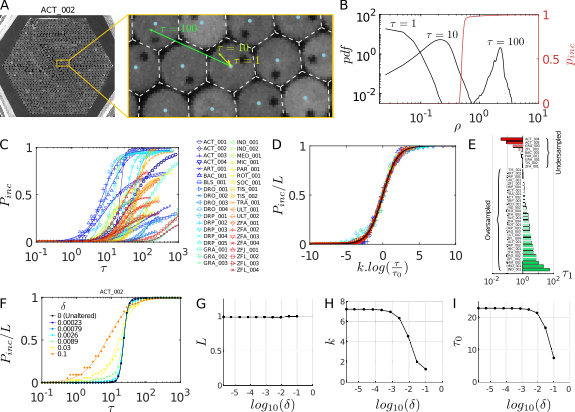
\includegraphics[width=1\textwidth]{part_1/assets/Figure_3.png}
    \caption{{\bf Characterization of the TD$^2$ dataset.}
        (\textbf{A}) Illustration of the dynamics at various timescales in$ACT\_002$. The Voronoï cells (dashed white) and the displacements of a particle at $\tau=1$, $10$ and $100$ are overlaid.
        (\textbf{B}) Geometric probability of incursion $p_{inc}$ (red) and distribution of the reduced displacement $\rho$ at three different timescales $\tau$ (black) in $ACT\_002$. The probability of incursion $P_{inc}$ is the intersection of the areas under the two curves.
        (\textbf{C}) $P_{inc}$ as a function of $\tau$ for the whole dataset (symbols). The solid lines are fits with a logistic function (see text).
        (\textbf{D}) Scaling of the reduced quantities $P_{inc}/L$ as a function of $k.log(\frac{\tau}
        {\tau_0})$ on the standard logistic sigmoid function (solid black).
        (\textbf{E}) Classification of the movies in the dataset by increasing values of $\tau_1$ as defined by eq.~(\ref{eq:Pinc_tau0}), with fitting parameters determined over a logarithmic scale for $P_{inc}$. Movies with $\tau_1<1$ are undersampled while movies with $\tau_1>1$ are oversampled.
        (\textbf{F}) Comparison of $P_{inc}(\tau)$ for different levels of degradation $\delta$ (symbols) and corresponding logistic fits (solid curves) in $ACT\_002$.
        (\textbf{G-I}) Evolutions of the fitting parameters $L$, $k$ and $\tau_0$ as a function of the degration $\delta$ in $ACT\_002$}
    \label{part_1:fig_3}
    \end{figure}

    \section{Parameters optimization}
    One may also want to determine the optimal tracking parameters, i.e., with a $P_{swap}$ close to 0 as possible. Provided that the ground-truth is known for at least one movie of a system, for example, by a careful manual post-processing. It is possible to leverage FastTrack's speed to explore the parameters space and minimize $P_{swap}$. The optimized parameters found that way can be used to track other similar movies with a minimal error rate. The workflow of the method is depicted in the Figure~\ref{part_1:fig_4}-A. As the exploration of the whole parameters space requires to perform at least thousands of trackings, such an approach is only made possible by the command-line interface (CLI) and the speed of execution of FastTrack.

    Let us first apply this approach to gain insight into the influence of $h_r$, i.e., the maximal distance allowed for an object to travel before considered lost. The Figure~\ref{part_1:fig_4}-B displays how $P_{swap}$ evolves as a function of $h_r$ for three recordings in the dataset. For low values of $h_r$, $P_{swap}$ is essentially imposed by the distribution of the objects' displacements since a high number of errors are generated when the objects are not allowed to move sufficiently. For higher values of $h_r$, the distribution of the distances to the neighbors (as defined by the Voronoï tesselation) starts to influence $P_{swap}$ as the algorithm becomes sensitive to incursions. It can also be more easily fooled by entries and exits at the boundaries of the region of interest when the number of objects in the scene varies.
    In between, for most recordings, there is a gap yielding the minimal probability of error. That is particularly true when the objects are densely packed, since the distribution of distances to neighbors is sharper, like for $DRP\_001$ where $P_{swap}$ drops to zero on a range of $h_r$. The acquisition framerate also has an essential role in this effect. With highly time-resolved movies, the distribution of displacements is shifted to the left (i.e., short distances), leading to a clear separation between the distribution of displacements and the distribution of the distances to the neighbors, resulting in low values of $P_{swap}$. In contrast, for poorly time-resolved movies like $ZFJ\_001$ the two distributions overlap, and $P_{swap}$ is always bound to high values.

    Similar analysis can be performed on the other tracking parameters. The Figure~\ref{part_1:fig_4}-C represents $P_{swap}$ as a function of both hard parameters $h_r$ and $h_t$ for $PAR\_001$, and a thin optimal segment appears. The Figure~\ref{part_1:fig_4}-D represents $P_{swap}$ as a function of the two soft parameters $s_r$ and $s_\alpha$, and an optimal ratio lies at $\frac{s_r}{s_\alpha} \simeq 0.63$. Altogether, a set of optimal parameters can be derived and used for the processing of similar recordings.

    \begin{figure}[h!]
    \centering
    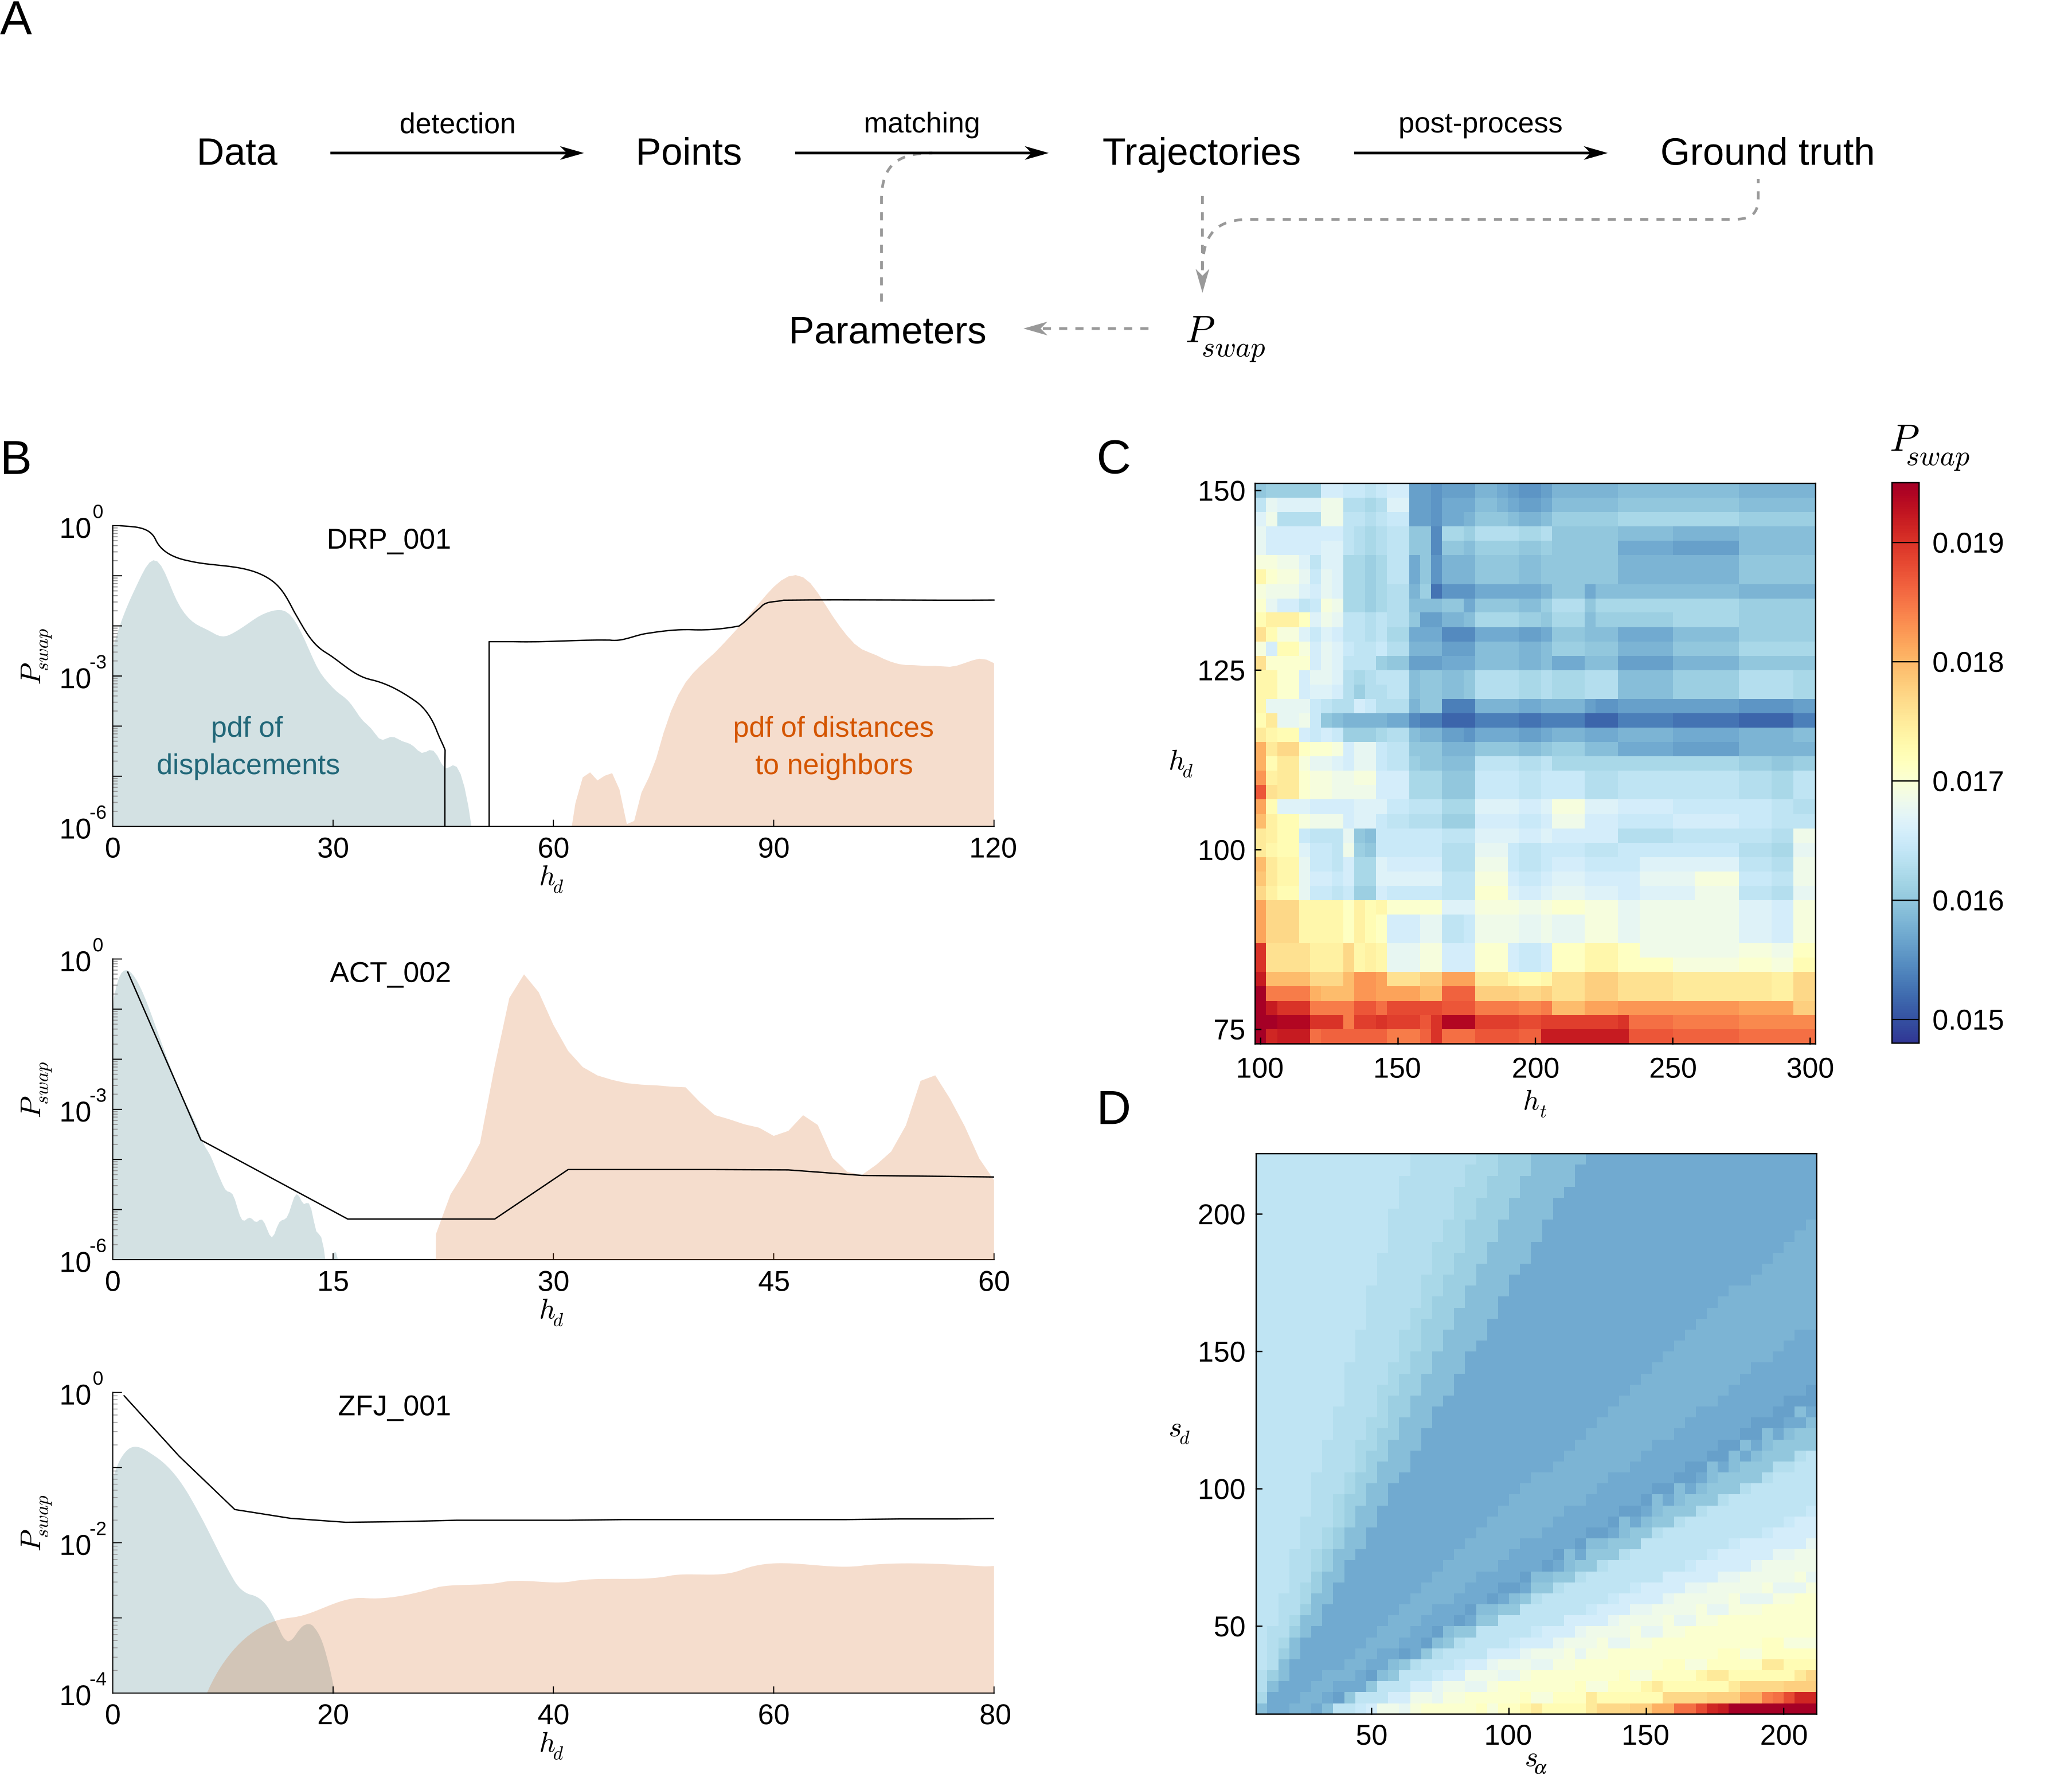
\includegraphics[width=1\textwidth]{part_1/assets/Figure_4.png}
    \caption{{\bf Optimization of tracking parameters based on $P_{swap}$.}
        (\textbf{A}) Scheme of the optimization workflow: on top of the detection/matching/post-process flow chart, the ground truth is used to compute $P_{swap}$ and create a feedback loop on the tracking parameters.
        (\textbf{B}) $P_{swap}$ (black) as a function of the maximal distance parameter $h_r$ (in pixels) for three typical recordings. Vertical lines for $DRP\_001$ indicate  that $P_{swap}$ drops to 0. The distributions of displacements between successive frames (blue) and of distances to the neighbors (orange) are also shown for comparison.
        (\textbf{C}) $P_{swap}$ as a function of the maximal distance parameter $h_r$ (in pixels) and the maximal disappearance time $h_t$ (in frames) for $PAR\_001$. Soft parameters are set to $s_r = 95$ and $s_\alpha = 60$.
        (\textbf{D}) $P_{swap}$ as a function of the normalization distance parameter $s_r$ (in pixels) and the normalization angle $s_\alpha$ (in degrees) for $PAR\_001$. Hard parameters are set to $h_r = 210$ and $h_t = 90$.}
    \label{part_1:fig_4}
    \end{figure}


\chapter{Perspective}
    In these chapters, we saw how we implemented a versatile and easy to use tracking software using open-source tools. Taking advantage of the GitHub Actions system, we automated the testing and the deployment of the software, increasing confidence, and promoting collaboration. We have shown that FastTrack can compete with state-of-the-art tracking software for many usages. At the same time, we compile a dataset of movies, allowing us to benchmark tracking software on a wide variety of systems. We classify the dataset based on the probability of incursion and, doing so, highlight a criterion to determine the optimal framerate of acquisition. We have finally shown how to determine the best set of tracking parameters by leveraging FastTrack's full capabilities.

    FastTrack's original approach, shifting the workload on the post-processing phase while keeping the pre-processing as light as possible, allows the use of FastTrack without insight into the system to track. The post-processing phase, mainly a swift checking of the tracking and small corrections, can be done directly inside the software in an interactive and ergonomic environment. FastTrack allows users to track movies quickly without any computer knowledge.

    FastTrack's approach does not prevent human inputs, mainly in the post-processing phase, to obtain a perfect tracking accuracy. It will be without inconvenience for many users who will need a human checking in any case. However, users who want a perfect tracking accuracy without human input will have to turn to other tracking software.

    It is important to note that the source code of FastTrack is available with a fully documented API. Power users can specialize the software with a custom detection phase or a custom cost function tailored to their system to circumvent any encountered limitation. The FastTrack command-line interface allows to embed the software in a high-level programming language like Python or Julia and integrate it inside an existing workflow.

    Overall, FastTrack gives any user the power to quickly analyze their movies on a relatively modest computer and power-user to build a custom-tailored software. The feedback we have encountered more frequently is how to analyze the tracking results. The standardized output leaves the user free to choose the analysis tool that he preferred. An answer to this request will be to develop analysis add-ons integrated into FastTrack if needed. These add-ons will be thematic (e.g., rats behavior, soft matter, etc.), and each one will have a specific set of functions to compute meaningful quantities specific to this domain and system. Another perspective that can be envisioned is to include the possibility of live tracking inside the software.


    \begin{appendices}
    \chapter{Voronoï diagram}
        \label{appendix_voronoi}
        \section{Definition}
        The Voronoï diagram is a partition of a spatial plan containing points into convex polygons, such as each polygon contains exactly one point.

        \begin{figure}[h!]
        \centering
        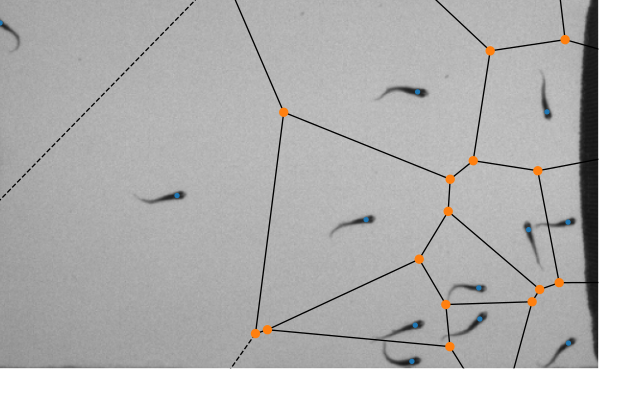
\includegraphics[width=0.75\textwidth]{part_1/assets/Appendix_voronoi.png}
        \caption{{\bf Exemple of a Voronoï diagram computed with one image of $ZFJ\_001$.} Voronoï vertices represented with orange point, seed points with blue points, finite Voronoï ridges with black lines, and infinite Voronoï ridges with dashed-black lines.}
        \end{figure}

        \section{Construction}
        In general position \footnote{An arrangement of points with no three collinear.}, the dual graph of the Voronoï diagram is the Delaunay triangulation. The Delaunay triangulation is a triangulation where every circumcircle is an empty circle. The circumcenters of Delaunay triangles are the vertices of the Voronoï diagram.

        \begin{figure}[h!]
        \centering
        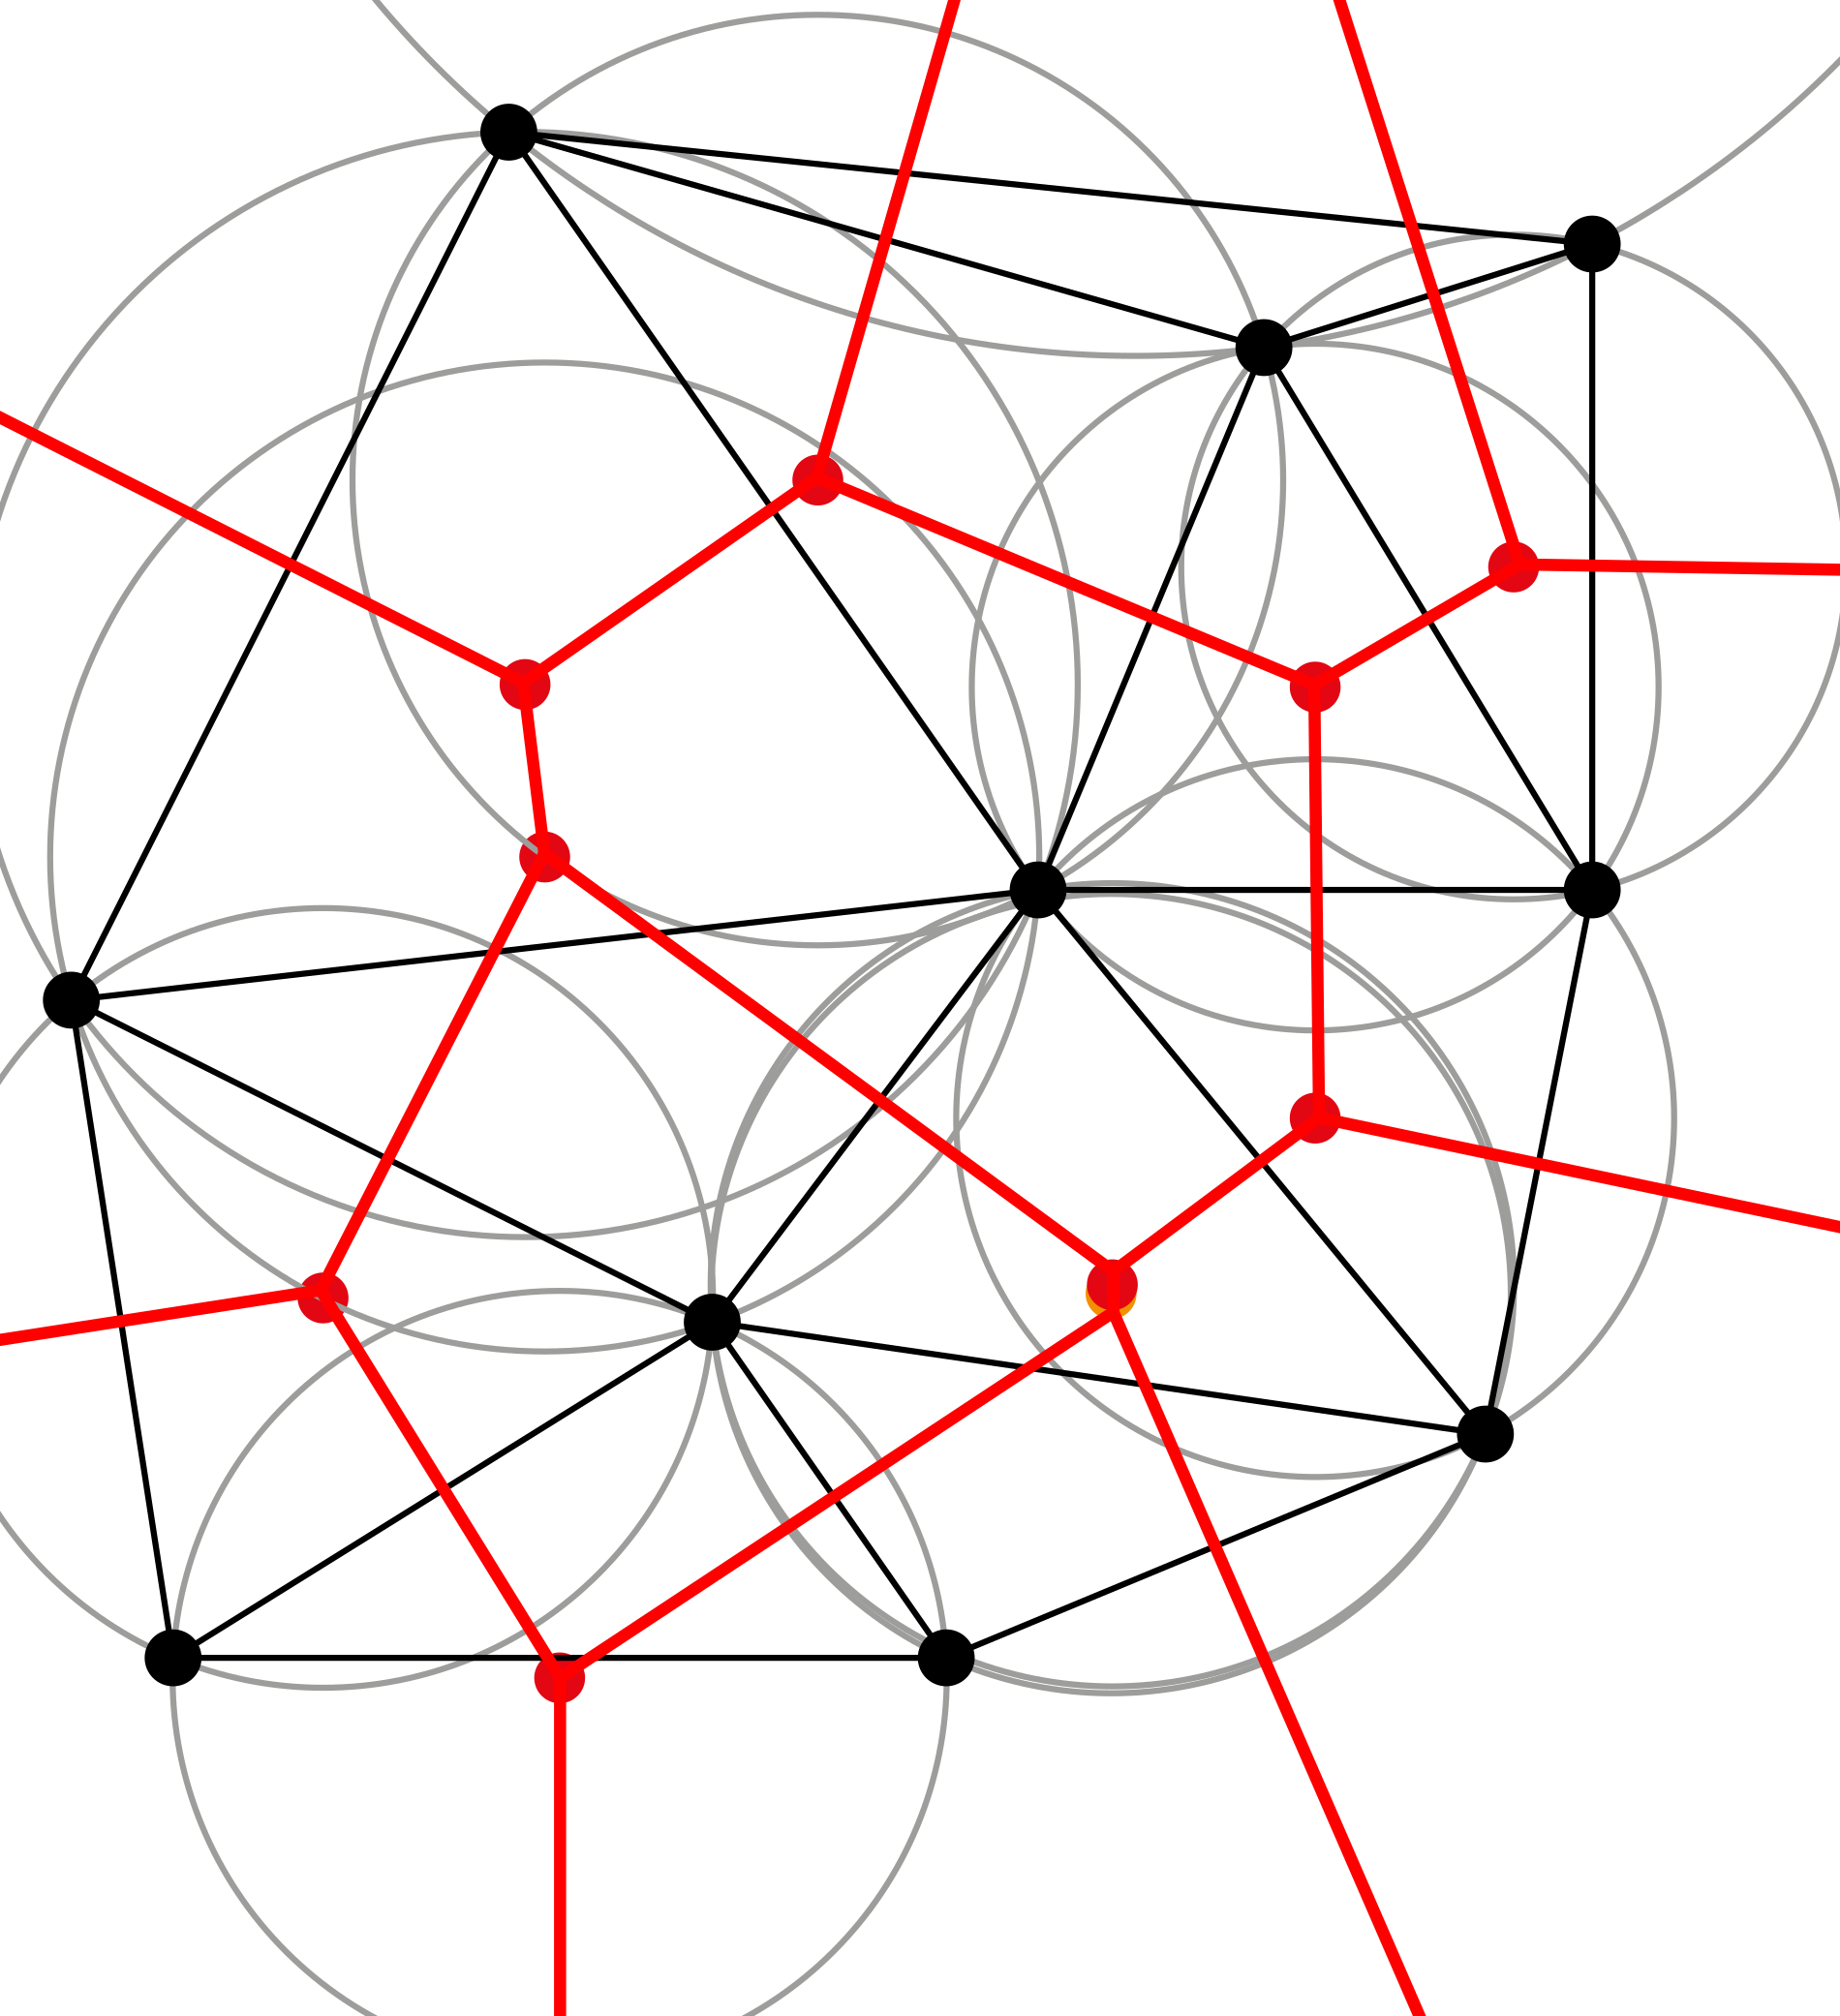
\includegraphics[width=0.5\textwidth]{part_1/assets/Appendix_delaunay.png}
        \caption{{\bf Delaunay triangulation and Voronoï diagram.} Delaunay triangulation in black, circumcircles in grey and Voronoï diagram in red.}
        \end{figure}

    \chapter{Hungarian algorithm}
        \label{appendix_hungarian}

        \section{Definition}
        The Hungarian algorithm is a combinatorial optimization problem that solves the so-called assignment problem in polynomial time \cite{kuhn1955hungarian}. Since 1957, it has been known as the Kuhn–Munkres algorithm \cite{munkres1957algorithms} after that, James Munkres reviewed it as strongly polynomial. First $O(n^{4})$, several implementations exist with a complexity of $O(n^{3})$ \cite{edmonds1972theoretical,tomizawa1971some,jonker1987shortest}.

        \section{Description}
        \paragraph{Problem:} We consider four jobs J1, J2, and J3 that need to be executed by four workers W1, W2, and W3, one job per worker. The objective is to minimize the total cost \footnote{\url{http://www.hungarianalgorithm.com}}. In this example, we choose the simplest form of the problem with a square matrix.

        $$\begin{matrix}
        & J1 & J2 & J3 & J4 \\
        W1 & 14 & 27 & 92 & 59 \\
        W2 & 38 & 43 & 50 & 17 \\
        W3 & 10 & 42 & 64 & 67 \\
        W4 & 88 & 32 & 83 & 89
        \end{matrix}$$

        Step 1: subtract the row minimum from each row:
        $$\begin{matrix}
        0 & 13 & 78 & 45 & (-14) \\
        21 & 26 & 33 & 0 & (-17) \\
        0 & 32 & 54 & 57 & (-10) \\
        56 & 0 & 51 & 57 & (-32)
        \end{matrix}$$

        Step 2: subtract the column minimum from each row:
        $$\begin{matrix}
        0 & 13 & 45 & 45  \\
        21 & 26 & 0 & 0   \\
        0 & 32 & 21 & 57   \\
        56 & 0 & 18 & 57   \\
        (-0) & (-0) & (-33)  & (-0)
        \end{matrix}$$

        Step 2: Covers all 0 with a minimum number of lines:
        $$\begin{matrix}
        \colorbox{BurntOrange}0 & 13 & 45 & 45 &  \\
        \colorbox{BurntOrange}{21} & \colorbox{BurntOrange}{26} & \colorbox{BurntOrange}0 & \colorbox{BurntOrange}0 & x  \\
        \colorbox{BurntOrange}0 & 32 & 21 & 57 &  \\
        \colorbox{BurntOrange}{56} & \colorbox{BurntOrange}0 & \colorbox{BurntOrange}{18} & \colorbox{BurntOrange}{57} & x  \\
        x &  &  &  &
        \end{matrix}$$

        Step 4: Find the smallest element $k$ not covered, substract $k$ to all uncovered elements and add $k$ to all elements that are covered twice:
        $$\begin{matrix}
        0 & 0 & 32 & 32  \\
        34 & 26 & 0 & 0  \\
        0 & 19 & 8 & 44  \\
        69 & 0 & 18 & 57
        \end{matrix}$$

        Repeat step 3 and 4 until there is exactly the same number of lines to covers all the 0 than the number of lines in the matrix. The optimal assignment is given by taking the set of 0 with one zero by line and by column, the cost by taking the value of these O in the initial matrix:
        $$\begin{matrix}
        \colorbox{BurntOrange}{0} & 0 & 24 & 24 \\
        42 & 34 & 0 & \colorbox{BurntOrange}{0} \\
        0 & 19 & \colorbox{BurntOrange}{0} & 36 \\
        69 & \colorbox{BurntOrange}{0} & 10 & 49
        \end{matrix}$$

        \noindent In this case the total cost is 127 with the assignment $\{J1; W1\}$, $\{J2; W4\}$, $\{J3; W3\}$ and $\{J4; W2\}$.

    \end{appendices}


\part{Dual}
\chapter{Introduction}

  \section{The chemical perception}
  The chemical senses are one the oldest sensory system \cite{yohe2018evolutionary}. They are the most used sensory modality and observed in a wide range of taxa, from unicellular \cite{bardwell2005walk} to mammalian. Some features and basics principles are highly conservated across phyla \cite{hildebrand1997mechanisms,yarmolinsky2009common}, and mediate several behaviors like predator avoidance, food-finding, and mating necessary to the survival of any species.

  Fish are immersed in their chemical environment at any time. This chemical environment is rich in information, and fish have evolved a complex sensory system to perceived and interpret these stimuli. For fish, chemical perception is mediated by three organs: olfaction (smell), gustation (taste), and a common chemical sense. Unlike terrestrial species, where substances perceived by smell and taste differ by the medium of transport of the molecules, fish taste and smell through the same medium: water. The solubility of compounds in water determines the type of compounds that can be transported and perceived. Therefore, chemical perception is non-directional and persistent. The distance traveled and the perceived concentration depend on the diffusion and convection of the medium, determining the perception threshold and the compound's residence time in the environment. The chemical perception is extremely specific, being contained in the molecular structures and the complex mixture of chemicals.

  Mechanisms of perception have been well studied for diverse fish species \cite{hara2012fish}, but highly complex directed behaviors like homing migration or food-finding are still poorly understood \cite{hansen2004chemosensory}. For example, fish can find food in complex environments like turbid and turbulent waters, where the perception is fragmented. Deciphering these mechanisms and their associated neural mechanisms will significantly advance the comprehension of the animal kingdom's most used sensory modality.

  One fish species, the zebrafish is an emerging model for studying goal-driven behaviors. At the larval stage (6 days post-fertilization), the animal is transparent, and it is possible to observe the brain activity with cellular resolution using light-sheet microscopy \cite{panier2013fast}. The development of virtual reality assays makes it technically possible to associate some neuronal networks' activity to the observed behavior. Using this technique; it was possible to gain insights into several behaviors, such as prey capture \cite{bianco2011prey}, optomotor response \cite{naumann2016whole}, phototaxis \cite{wolf2017sensorimotor}, rheotaxis \cite{olive2016rheotaxis}, and thermotaxis\cite{haesemeyer2019convergent}.

  The development and functioning of the fish sensory organs, particularly in the zebrafish, have been well characterized. However, there are few behavioral studies on chemical perception and chemically-oriented navigation. Several milestones have to be achieved before using virtual reality assays to study chemically-driven navigation. One needs to find and characterize products that elicit robust and attractive behaviors. The space of possibilities will be vast, and completing this task necessitates a high-throughput setup to explore combinations of products, concentrations, and fish ages. In a second time, when a product that elicits a robust and attractive response will be characterized, studying realistic chemically-driven navigation will require a setup capable of reproducing turbulent flows where the fish is immersed in a complex chemical environment with fragmented perceptions.

  In the next sections, we will present in detail the sensory organs of the zebrafish and review experimental setups used to characterize the chemical perception of the zebrafish at the larval and adult stage. Then we will present two experimental setups that we build: Dual, a high-throughput screening device capable of assessing the chemical preference of larval and adult zebrafish; The Tropical River, a setup capable of generating controlled flows that can be used to study chemically-driven navigation. Finally, we will present some results that we obtain using the Dual setup.


    \subsection{Olfaction}
    The olfactory organ of the fish, see Figure~\ref{olfactory_schematic}, consists of two structures located in the animal's snout \cite{hara2012fish}. Each structure consists of a cavity called the olfactory chamber connected to the outside by an entrance and an exit nostril. The inside of the olfactory chamber is lined with the olfactory rosette consisting of two rows of olfactory lamellae. The olfactory epithelium, where the olfactory receptors are located, is placed on these lamellae. The olfactory organ's exact organization and position can vary depending on the fish species, for example, with the addition of a ventilation cavity as an extension of the olfactory cavity.

    \begin{figure}[h]
      \centering
      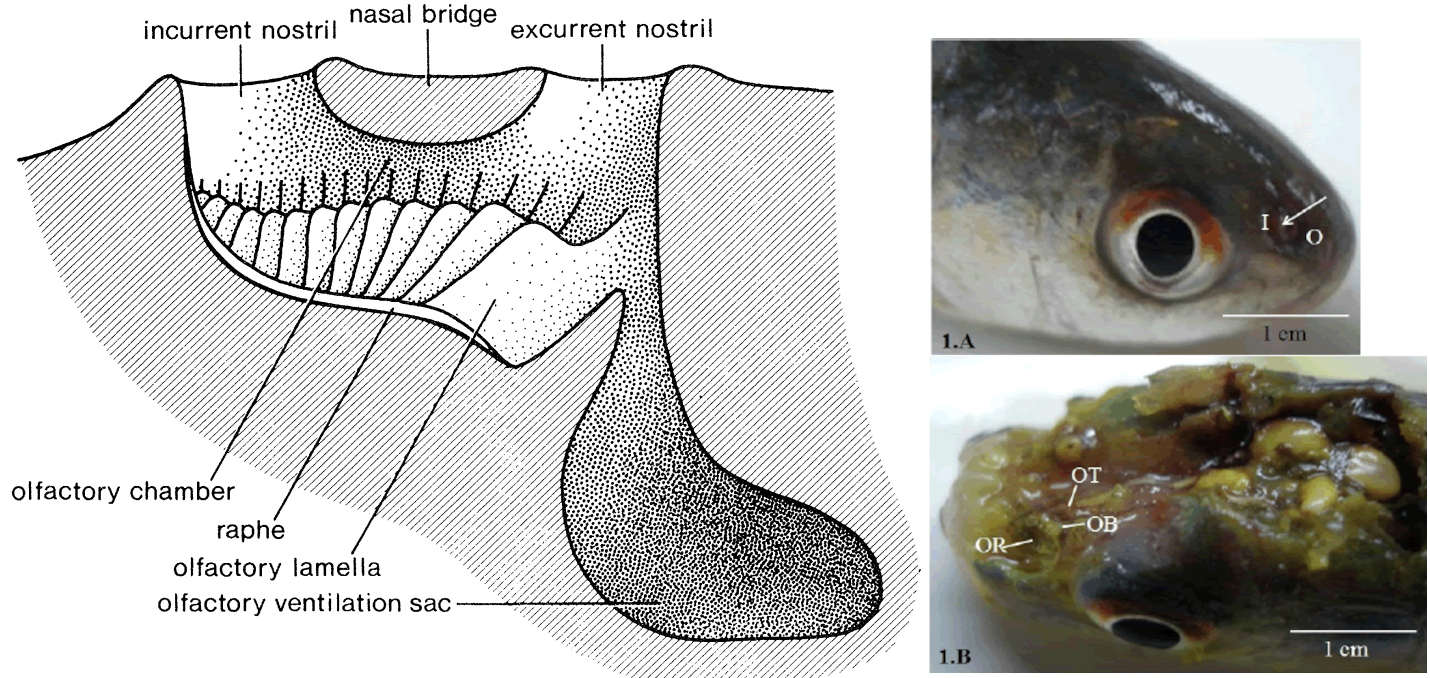
\includegraphics[width=10cm]{part_2/assets/olfactory_schematic.png}
      \caption{Olfactory system, reproduced from \cite{hara2012fish}.}
      \label{olfactory_schematic}
    \end{figure}


    The olfactory epithelium has a $100\mu m$ thick pseudostratified columnar structure \cite{hara2012fish}. It can be separated into a sensory and a non-sensory epithelium. The sensory epithelium consists of three types of cells: receptor, supporting, and basal cells; the non-sensory epithelium of goblet cells and non-sensory ciliated cells. There are five receptor cells implicated in the olfactory perception: ciliated cells, microvillous cells, crypt cells \cite{ichikawa1977fine,hansen2005diversity}, kappe cells \cite{ahuja2014kappe}, and pear-shaped cells \cite{wakisaka2017adenosine}. They express olfactory receptors of the OR, V1R, V2R, and TAAR families. Receptor cells have various sizes, shapes, and distribution inside the epithelium see Figure~\ref{olfactory_schematic_full}.

    \begin{figure}[h]
      \centering
      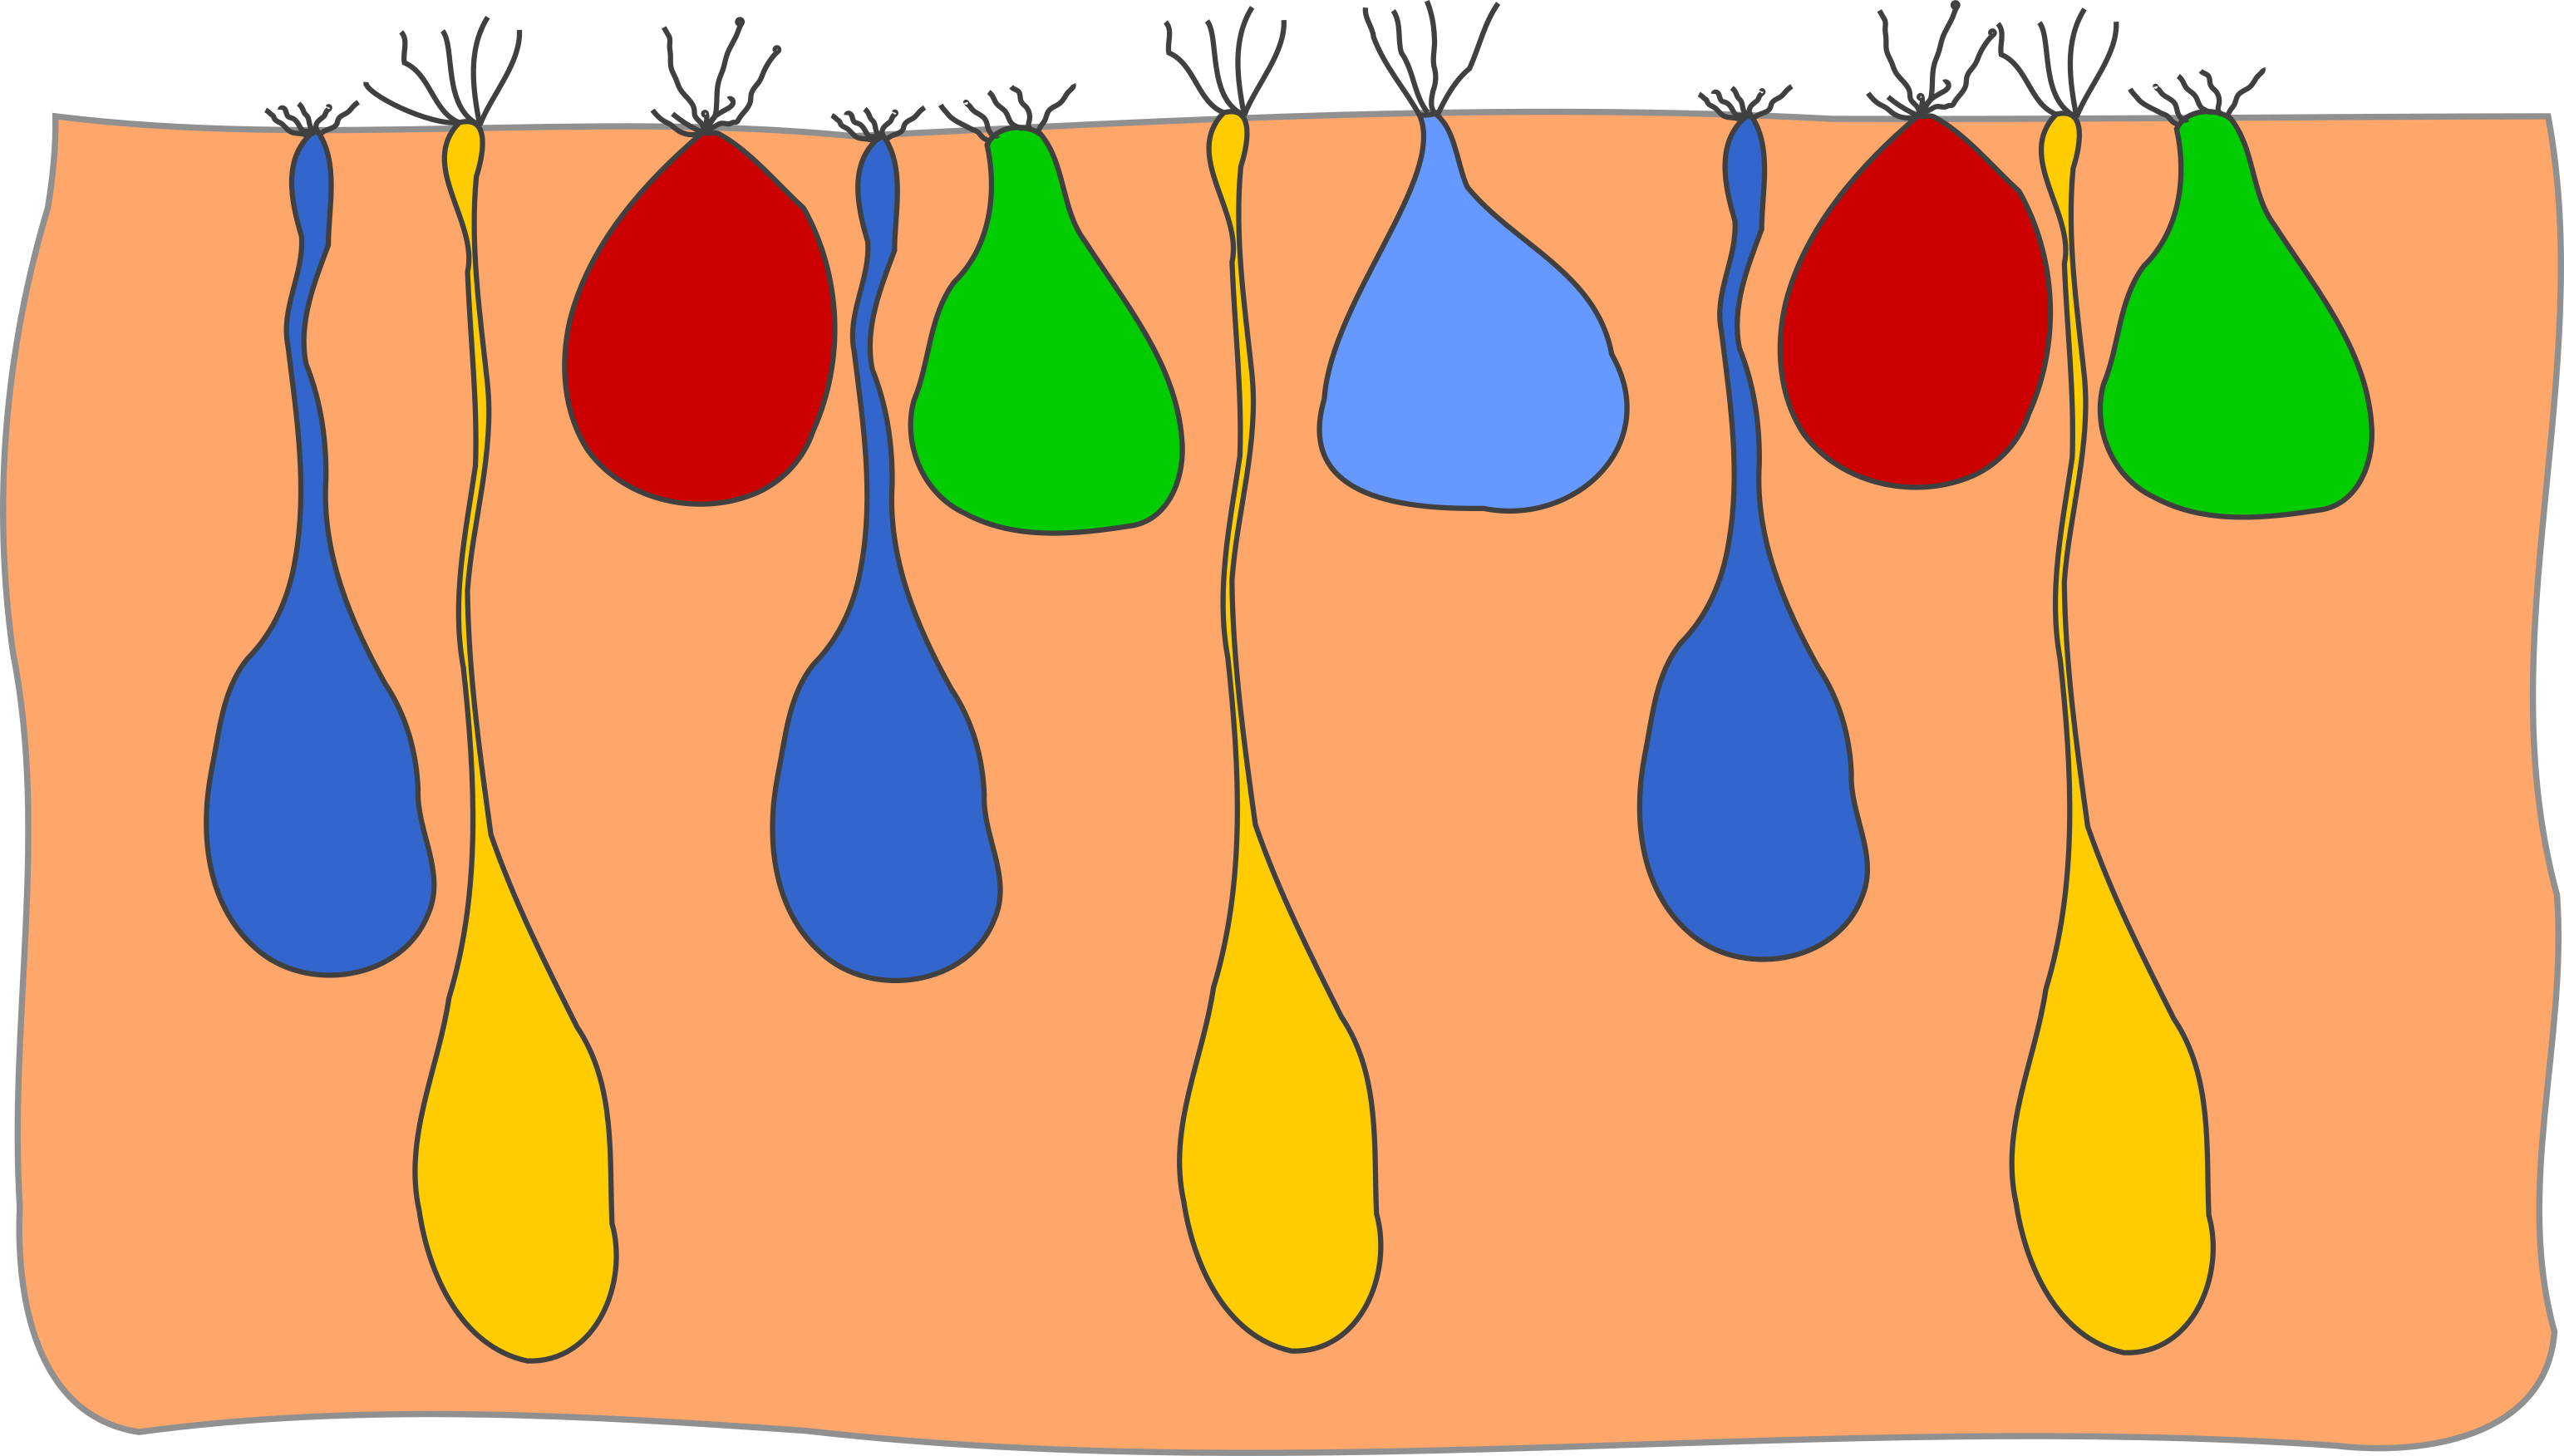
\includegraphics[width=10cm]{part_2/assets/olfactory_schematic_full.png}
      \caption{{\bf Schematic representation of the olfactory epithelium.} Ciliated neuron in yellow with round somata, slender dendrite, and cilia. Microvillous neuron in dark blue with microvilli at the surface. Crypt neuron in red with ovoid shape, microvilli, and cilia. Kappe neuron in green with microvilli. Pear-shaped neuron in light blue with cilia.}
      \label{olfactory_schematic_full}
    \end{figure}

    Receptor cells project directly into the olfactory bulb located in the brain, in turn sending signals to the telencephalon and diencephalon \cite{miyasaka2009olfactory}. The olfactory bulb in the teleost is a structure of four concentric layers: olfactory nerve layer (ONL), glomerular layer (GL), mitral cell layer (MCL), and internal cell layer (ICL). The olfactory information is transmitted by the receptor cells to the olfactory bulb \cite{nikonov2001electrophysiological} then in the forebrain \cite{nikonov2005beyond} as a topographical odor map. The olfactory bulb's neuronal connections have been particularly studied in the zebrafish \cite{hansen1998peripheral,kermen2013neural}, the olfactory bulb comprised approximately 20 000 neurons \cite{friedrich2009processing} and 140 glomeruli\cite{braubach2012distribution}. Each receptor cell expresses only one type of olfactory receptor \cite{serizawa2004one,barth1997noncoordinate,weth1996nested,sato2007hierarchical} except in a subpopulation of olfactory sensory neurons \cite{sato2007hierarchical}. Cells expressing the same receptor are projecting into the same olfactory bulb glomeruli \cite{sato2005mutually}. Glomeruli responding to similar odorants are grouped into domains within the olfactory bulb, forming chemotopic maps. Odorants can activate glomeruli outside their domain, leading to a fragmented map inside the olfactory bulb \cite{friedrich1998chemotopic}. Moreover, the odor encoding is hierarchized with first-order features encoded by large domains and second-order features by local activity patterns within the domain \cite{fuss2001odorant,korsching2001odor}.

    The olfactory bulb projects into two higher brain structures, the telencephalon (Dp and Vv) and the diencephalon (habenula, posterior tubercle, and hypothalamus). The neuronal activity evoked by olfactory cues in these areas is currently poorly understood \cite{}.

    In the zebrafish \cite{hansen1993development,miyasaka2013functional}, the olfactory organ develops from the olfactory placodes at the 6-10 somites stage (about 15 hours post-fertilization) of the embryonic development. The olfactory cavity begins to appear at the 28-30 somites stage (31 hours post-fertilization). Approximately 50 hours post-fertilization, the olfactory epithelium and the receptor cells appear. When the embryo exits from the chorion at 4 days post-fertilization, the olfactory organ continues its morphological development, but the cytological organization remains largely unchanged. At 40 days post-fertilization, the bridge between the entrance nostril and the exit nostril is completely formed, separating the currents going out and coming in from the olfactory cavity. The addition of lamellae to the olfactory rosette continues throughout the life of the zebrafish.

    \subsection{Gustation}
    The gustatory organ of fish is composed of taste buds which are not localized in a single location but are rather spread all over the body surface, which directly contact chemical substances. Taste bud histology has been studied for different fish \cite{kapoor1976gustatory,fishelson2004taste,reutter2000heterogeneity,reutter1991ultrastructure,reutter2012taste}, and they usually have an elongated and ovoid shape, see Figure~\ref{gustatory_schematic}. They sit on a small dermal papilla and extend throughout the epidermis' thickness protruding from the surface. The taste bud is constituted of a sensory (dark cells with microvilli and light cells with one large microvillus) and a non-sensory (Merkel‐like basal cells) epithelium. The apical ending of the sensory cells that protrude from the epithelium is called the receptor field and is covered with a mucous cap. The number of sensory cells in a taste bud varies considerably depending on the fish species.

    Taste buds are distributed all over the fish's body, especially in the mouth, on the lips, and the skin. Their distribution and concentration vary according to the species. Three different cranial nerves innervate them: facial (VII), glossopharyngeal (IX), and vagal (X). The facial nerve transmits information from the extra-oral taste buds; the glossopharyngeal nerve transmits information from inside the oral cavity; the vagal nerve transmits information from inside the oropharyngeal cavity. The taste system is anatomically divided into two distinct parts: nerves IX and X projecting into the brain's vagal lobe and nerve IV into the facial lobe. Connections to higher areas of the brain differ slightly from one species to another. It has been shown in Ictalurus nebulosus \cite{atema1971structures} that these two systems have distinct roles in fish feeding behavior.

    \begin{figure}[h]
      \centering
      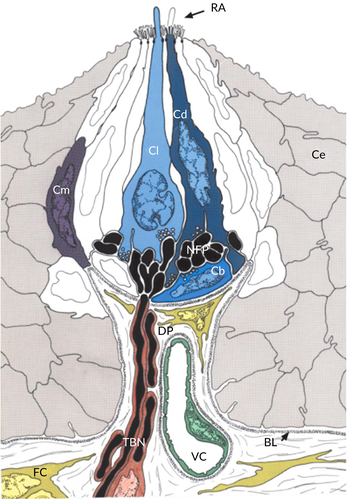
\includegraphics[width=8cm]{part_2/assets/gustatory_schematic.png}
      \caption{\textbf{Schematic drawing of a typical taste bud of teleosts from \cite{hansen2002taste}.} Dark cells (Cd), light cells (Cl) and Merkel‐like basal cells (Cb). Marginal cells (Cm). Ce epithelial cells. Dermal papilla (DP). (TBN) taste bud nerve. (BL) basal lamina. (RA) receptor area. (VC) capillary vessel.}
      \label{gustatory_schematic}
    \end{figure}

    In zebrafish \cite{ohkubo2005distribution}, the taste buds (approximately 2 200) are located on the lips, in the oropharyngeal cavity on the barbels, and on the head's ventral and dorsal side. Each taste bud contains 20 to 23 cells. Projections of the zebrafish gustatory system have been studied in detail \cite{yanez2017gustatory} and form a complex network that can be summarized graphically see Figure~\ref{gustatory_connection_schematic}.

    \begin{figure}[h]
      \centering
      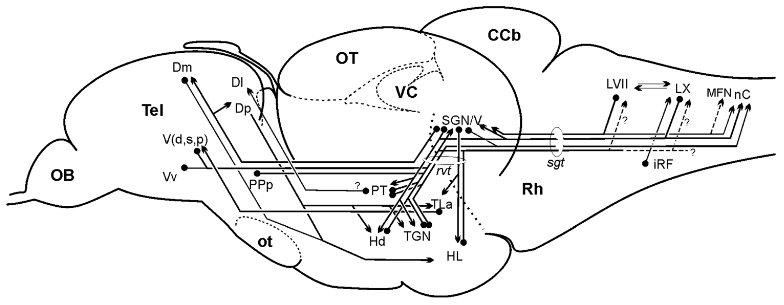
\includegraphics[width=10cm]{part_2/assets/gustatory_connection_schematic.png}
      \caption{\textbf{Gustatory system of the zebrafish}. Neuronal connections of the fish taste system reproduced from \cite{yanez2017gustatory}.}
      \label{gustatory_connection_schematic}
    \end{figure}

    The development of the gustatory organ has been studied in the zebrafish \cite{hansen2002taste}. The first taste buds appear at 3 or 4 days post-fertilization and are located on the lips and the gill arches. The taste buds in the mouth and oropharyngeal cavity appear 4 to 5 days post-fertilization. The taste buds on the head do not appear until 12 days post-fertilization, and it is not until the juvenile stage (30 to 40 days post-fertilization) that the barbels appear. Note that the appearance of the taste buds coincides with the appearance of feeding in the larvae.

    \subsection{Common chemical sense}
    Fish also have a third chemical sense called the common chemical sense. It consists of bipolar neurons called solitary chemosensory cells (SCCs) embedded in the epidermis. Their distribution and number vary greatly depending on the species. Therefore their study is difficult, and their function and neuronal connections are poorly understood.

    In the zebrafish \cite{kotrschal1997ontogeny}, SCCs have been described as a set of 2-7 villi of 0.5 to 1 $\mu m$ length emerging from the cell body at embryo and larval stage.  In adults, SCCs possess a single villus of $3\mu m$ length.

    The first SCCs appear at 3 days post-fertilization. Their density increases until 25 days, where their number stabilizes at $1.10^6$ per $mm^2$ with 2 to 5 times more SCCs on the zebrafish's head than on its body.


  \section{Behavioral studies}
    \subsection{Behavior}
    The olfaction and gustation have been shown to mediate several fish behaviors. It is not easy to distinguish the contribution of each sense in the observed behavior. Moreover, this contribution seems to be dependent on fish species.

    A well known and impressive behavior encountered in many fish species is the homing migration. A typical example is salmons that perform three migratory phases throughout their life. One of them, the upstream migration from the ocean to their home stream, has been shown to rely on an olfaction imprinting \cite{stabell1992olfactory,hasler1983olfactory}. Little is known about the imprinting mechanism, but experiments suggest that it relies on a mixture of odors perceived during the juvenile stage in the fish's home stream.

    Feeding is one of the most important behaviors. It relies on several senses for food detection, and selection \cite{pavlov1990sensory}. A stereotyped behavioral sequence was shown to exist \cite{atema1980chemical} consisting in a step of arousal mainly mediated by olfaction \cite{bateson1890sense}, then a step of localization of the food mediated by chemical and visual cues. The last step of ingestion is triggered primarily by the gustation \cite{atema1980chemical}. The impact of each sensory modality varies significantly with the species. For example, the yellow bullhead has the entire feeding sequence mediated by taste, whereas ictalurid catfish prey detection was abolished when olfaction was blocked. The chemical substances that attract fish depend on the species \cite{atema1980chemical}, and response to a mixture is higher than isolated compounds in general.

    Olfaction \cite{tavolga1956visual} as well as the gustatory system \cite{de1983influence} has been shown to play an essential role in reproduction. Non-anosmic males exposed to water taken from a tank with a gravid female developed courtship behaviors, except for some species like the three-spined stickleback where the gustation can replace the olfaction. Complete courtship repertoire necessitated the presence of other sensory cues.

    Fright reaction occurred when a fish perceived an alarm substance secreted by a conspecific. This reaction differs between species and involves seeking cover, rapid swimming, or freezing. It is accepted to be mediated by olfaction \cite{frisch1942schreckstoff,speedie2008alarm,doving2009alarm}, but other sensory cues are not ruled out.

    The zebrafish has been used to connect the behavioral and neuronal response to diverse stimuli: visual stimuli \cite{}, temperature \cite{}, and balance reflexes \cite{}. Most of the works to date focus on developing the model for pharmacological safety screening \cite{cassar2019use}, drugs addiction \cite{klee2012zebrafish}, and ecology \cite{dai2014zebrafish}, enabling a low cost and genetically manipulable model. Behavioral studies of the chemical perception of zebrafish, adults, or at the larval stage have been done through various experimental assays that we will be presented in the following sections.

    \subsection{Conditioned place preference}
    The conditional place preference (CPP) experiment is a type of Pavlovian conditioning. Pavlovian conditioning consists of associating a conditioned stimulus (generally neutral) with an unconditioned stimulus. After learning, the animal exhibits a conditioned response to the conditioned stimulus when presented alone. The most classic example is associating a bell's sound (conditioned stimulus) to the release of a food smell (unconditioned stimulus). After learning, the animal can respond to the bell's sound alone, as demonstrated by Ivan Pavlov on dogs \cite{pavlov1903experimental}.

    This approach was applied to test the response to various chemical stimuli in adult zebrafish \cite{mathur2011conditioned}. The experiment follows a classical 3-step design. The first step is to evaluate the fish's base-line preference. The animal is placed in an aquarium with two or three distinct areas differentiate by walls' pattern and color, see Figure~\ref{cpp_schematic}. The fish is tested to find out which side it naturally prefers. In this experiment, the distinctive walls' pattern and color play the role of the conditioned stimulus. The second step is the conditioning phase. The fish is restrained to its least preferred area, and the substance to be tested injected into the water (unconditioned stimuli). The last step consists of repeating the first step to assess the change in preference of the animal.

    Several chemical substances have been tested using this method \cite{blaser2014experiments,collier2013utility,tzschentke2007review}. Notably, a strong and robust cocaine-induced CPP response in WT zebrafish was shown \cite{darland2001behavioral}, with $85\%$ of the fish changing preference to a cocaine concentration of $10mg.L^{-1}$ and lower and higher concentrations resulting in a lower response. A positive response of adult zebrafish to a single ethanol exposure was shown \cite{mathur2011preference} in a similar experimental setup. It should be noted that this is also the first study to use an automated tracking system to calculate animal preference. Zebrafish showed a positive response for D-amphetamine \cite{ninkovic2006genetic, ninkovic2006zebrafish}, salvinorin A \cite{braida2007hallucinatory}, cocaine \cite{braida2007hallucinatory}, spiradoline \cite{braida2007hallucinatory}, nicotine \cite{kedikian2013behavioral} and ethanol \cite{kedikian2013behavioral}.

    We see that CPP has been used extensively to study the response to chemical stimuli in zebrafish. There is a strong emphasis on products that cause addictive pathologies in humans. Nevertheless, this protocol has several limitations, the most important being that it involves several systems of perception as well as memory. During the conditioning phase, the learning is based on the visual perception of the environment (pattern on the aquarium walls), the chemical perception of the tested compound, the association of the two stimuli coming from different sensory organs, and the memorization of these perceptions. Secondly, the time window to perform the experiment (minimum two days) is a hindrance to use the CPP to study the effect of many chemicals in a high-throughput manner. TODO

    \begin{figure}[h]
      \centering
      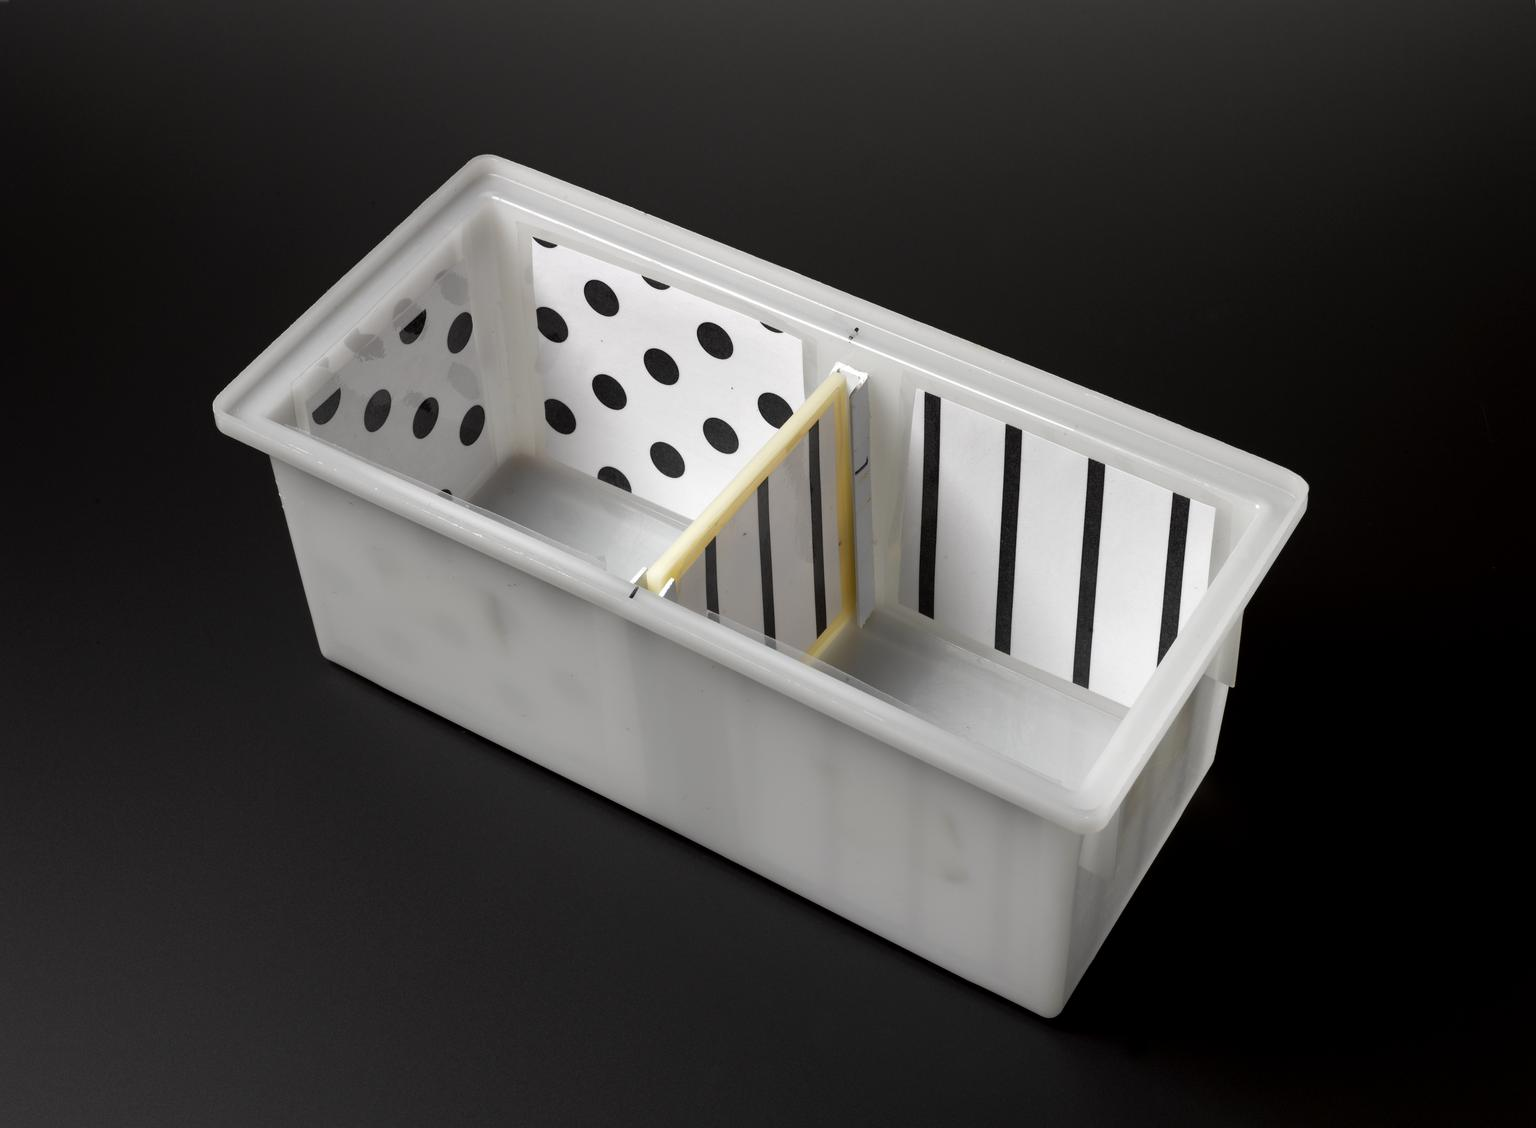
\includegraphics[width=0.8\textwidth]{part_2/assets/cpp.jpg}
      \caption{\textbf{Conditioned place preference apparatus}.  CPP setup for zebrafish reproduced from Brennan Caroline, Queen Mary University of London. The middle wall is removed for the first and third step of the CPP.}
      \label{cpp_schematic}
    \end{figure}

    \subsection{Multi well-plate}
    A widely used experimental apparatus to assess chemical compounds' effect on zebrafish larvae and embryos is the well-plate device \cite{rennekamp201515}. One or more larvae is placed in each well in a bath of a chemical. Larvae are then recorded swimming in the chemical compound, and the kinematic parameters of the animal are extracted. In the case of embryos, development is monitored after exposure. The advantage of this technique is that it requires only a single experimental apparatus. It quickly produces a large amount of data with well-plate with up to 48 wells per plate. Software already exist to extract automatically relevant behavior parameters from video recordings \cite{zhou2014quantification}.

    With this kind of assay, many chemical compounds have been tested \cite{sallinen2009mptp,rihel2010zebrafish,kokel2010rapid}, as well as seizure liability \cite{winter2008validation}, and several behaviors \cite{farrell2011evaluation, shen2020rapid,schnorr2012measuring,pelkowski2011novel}.

    The well-plate device allows for an easy and automatic high-throughput screening of chemicals. Turnkey commercial solutions like the Zebrabox from ViewPoint exist, and custom setups are relatively easy to build. However, this system suffers limitations like the fact that one can not assess the fish preference. Precisely controlled exposure, or repeated exposure through cycles of exposition/flushing, are not available. Therefore this system is not adapted to investigate fish's chemical preference and chemical-driven navigation.

    \begin{figure}[h]
      \centering
      \includegraphics[width=0.4\textwidth]{part_2/assets/well.png}
      \caption{\textbf{A Zebrabox from Viewpoint}.  Zebrabox, the most used solution for well-plates experiments.}
      \label{zebrabox}
    \end{figure}

    \subsection{Direct introduction}
    Some authors have tried to quantify chemically induced behavior by introducing a chemical compound directly into the tank and looking at the percentage of time spent close to the source. Notably, an attraction concentration-dependent to adenosine for adult zebrafish\cite{wakisaka2017adenosine} and to GCDA and nicotine for zebrafish larval \cite{krishnan2014right} was shown. A strong aversion to cadaverine, an odor associated with decomposing bodies, was shown using a tank with a single compartment or a tank with two compartments and an intermediate zone where the fish can changes compartment \cite{hussain2013high}, see Figure~\ref{diffusion_setup}.

    Very easy to implement, these types of experimental devices lack control in the concentration perceived by the animal. Diffusion and advection are neglected in the experiment, and the concentration is poorly known and not reproducible. The effects of diffusion and advection were mitigated \cite{hussain2013high} by adding a wall separating the two zones Figure~\ref{diffusion_setup}.F, always leaving uncertainty in the intermediate zone. Moreover, these setups exclude the realization of long experiments due to the homogenization of the product.

    \begin{figure}[h]
      \centering
      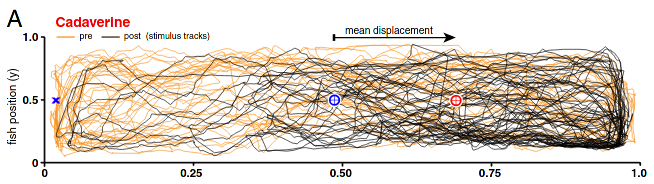
\includegraphics[width=1\textwidth]{part_2/assets/diffusion.png}
      \caption{\textbf{Diffusion setups from \cite{hussain2013high}}. \textbf{A.} One channel diffusion setup, blue cross: chemical introduction point. \textbf{F.} Two channels setup.}
      \label{diffusion_setup}
    \end{figure}

    \subsection{Flow}
    Another type of device that allows the product's concentration inside the tank to be quickly changed was used on adult zebrafish \cite{kermen2020stimulus}. Like in the multi-well experiment, chemically induced behavior changes were monitored by the animal's kinematic parameters.

    Several food odors were shown to produce a significant increase in speed and number of bursts; social odors from conspecific produced a similar response; alert odors result in a dive to the bottom of the tank and an increase in frozen time; decomposition odors result in more turns. The critical points noted with this device is the inter-and intra-experimental variability. The authors showed that less than a third of the odors used in the study produce reproducible results between trials of the same individual. Some odors such as cadaverine, blood, skin, and food odors resulted in inconsistent responses for the same individual. Most odors produce poorly reproducible results for different fish.

    \begin{figure}[h]
      \centering
      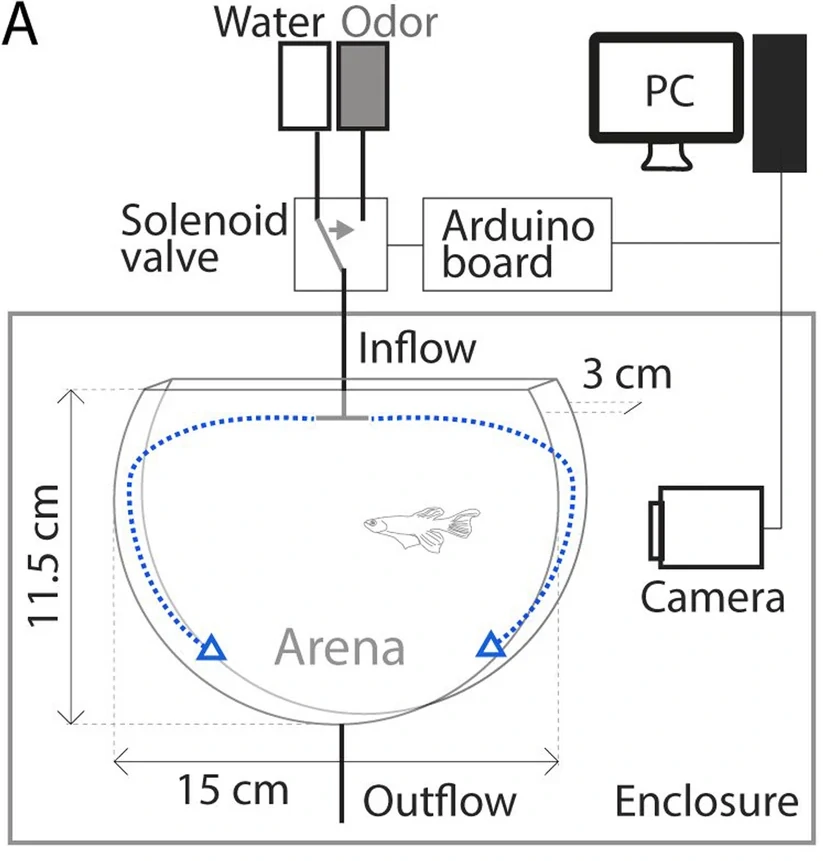
\includegraphics[width=0.5\textwidth]{part_2/assets/flow_1.png}
      \caption{\textbf{Flow setups from \cite{kermen2020stimulus}.}}
      \label{flow_1_setup}
    \end{figure}

    This setup novelty is to allow adult animals to evolve realistically in a 3D environment and to have a better knowledge of the concentration perceived by the animal than in a diffusion setup. Therefore, direct preference assessment is not accessible, and comparisons with existing quasi-2D setups like the well-plate are difficult.

    A more controlled setup to study chemical preference in fish is the underflow device. The first mention of this type of device dates back to 2013 \cite{readman2013fish}. In this setup, the tank is separated into two distinct compartments using a laminar flow, see Figure~\ref{flow_0_setup}. The animal can then choose between the two compartments during the experiment without any constraint, and the experimenter can put a chemical to test on one side. The interface between the two compartments self-heal with a characteristic time depending on the flow velocity. The time spent on each side, the number of interface crosses, and the animal's kinematic parameter are extracted from video recordings to assess the fish's preference.

    Several psychoactive substances have been tested on adult zebrafish \cite{abreu2016acute, abreu2016behavioral} and showed attraction by diazepam, fluoxetine, risperidone, and buspirone; neutral response to ethanol and clonazepam; an aversion to acid pH, two food odor extracts, and conditioned water took from a tank with chemically and physically stressed fish.

    This setup has several advantages. The concentration of the product is perfectly known because the diffusion and advection are mitigated and controlled by the flow. The preference of the fish can be directly measured as the fish can choose freely to go inside or outside the product. Long experiments can be performed with this setup, and product delivery precisely controlled in time. However, some disadvantages remain, like the absence of a standardized or turnkey setup and the volume of water and chemicals required that can be high.

    \begin{figure}[h]
      \centering
      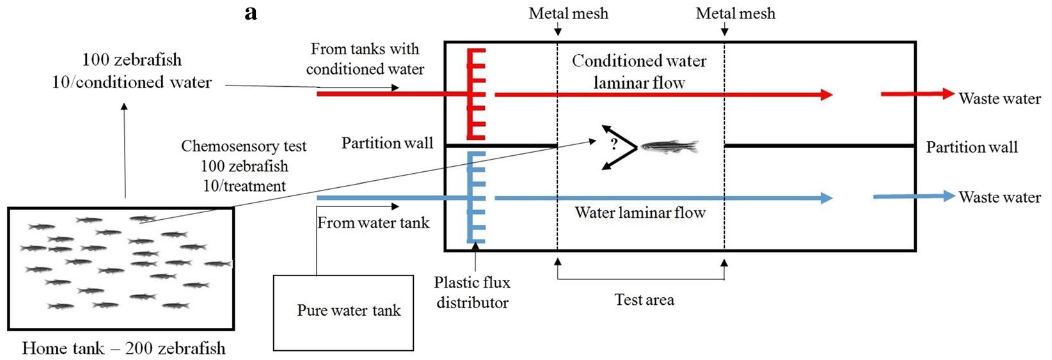
\includegraphics[width=1\textwidth]{part_2/assets/flow_0.png}
      \caption{\textbf{Flow setups from \cite{abreu2016behavioral}.}}
      \label{flow_0_setup}
    \end{figure}

    From this overview of the scientific literature, we see that the study of chemical perception and behavioral response to chemical stimuli is not standardized.Direct comparisons between studies carried out in various independent laboratories are not easily possible. In this context, we have developed Dual, an open-source, easy to replicate, low cost, do it yourself, and scalable experimental setup. Using the underflow principle, Dual allows studying chemical preferences in larvae and juvenile zebrafish in a standardized, high-throughput, and comparable way.

\chapter{Experimental setups}
  To study the young zebrafish chemical perception, we build two complementary setups: one to screen products, the other to recreate more natural flows, and studies the chemically-driven navigation. The first, named Dual was designed and build from scratch. The latter, The Tropical River was adapted from a previous experiment.

  \section{Dual}
  The design and implementation of experimental setups that are high-throughput, bias-free, and scalable are essential to behavior characterization. We present Dual, a high-throughput experimental setup that is easy to build, scalable, and costs less than 1 500 USD.

  \subsection{Overview}
  Dual is an underflow system built on the same principle than \cite{readman2013fish}. It consists of creating two compartments in a tank through a laminar flow without a physical separation. As we have seen previously, this system allows a rigorous knowledge of the compound's concentration to which the animal is subjected. Diffusion and advection due to the water movements caused by the fish are avoided. The interface between the two compartments is well defined and self-healing when disturbed, with a characteristic time depending on the flow rate.

  To create the laminar flow, Dual uses a system of four syringes, coupled two by two: when two syringes push, two syringes pull, see Figure~\ref{dual_mechanical}. The syringes are connected to the inputs and outputs of a millifluidic chip and generate a laminar flow with constant volume by having two syringes injecting at one side and two aspirating at the other side. Thanks to a computer-controlled manifold composed of six microvalves, each syringe can be filled independently. One can then build an experimental protocol by stacking several filling and injection cycles and choosing what to fill the syringes with. The fish is placed inside the millifluidic chip, see Figure\ref{dual_chip_visu}.

  For example, to assess fish preference, one can first create a cycle with water on the two sides as habituation and control. Then add a cycle with a chemical on one side and water on the other side to study the fish preference. Another example is to fill the two sides with a chemical for a given amount of time and then clean the system with water on the two sides, reproducing the type of experiment performed with the multi well-plate device. A large variety of experiments can be designed with none or few setup modifications.

  Dual is a custom-built system using several components stemming from the makers' community (Openbuilds, Markerbeam, Arduino), which allows great flexibility in the conception and fast iteration to adapt the project if necessary. All the components, blueprints, and other CAD files needed to build and assemble Dual are available in the appendixes. Dual can be built at a low-cost (see the bill of materials~\ref{bom}) without prior knowledge of mechanics or electronics. The tools necessary for realizing Dual can be found in a FabLab and necessitate little formation.

  \subsection{Construction}
  For the construction, Dual can be separated into five main parts. The mechanical system comprised the static structures, the motor, and moving parts. The millifluidic system is constituted of the millifluidic chip, the microvalves, the syringes, and connecting tubes. A camera, lens, infrared filters and LEDs form the imaging system. The electronic system is a custom PCB controlling the motor and the microvalves. Finally, a software that controls all the setup automatically.

  \subsubsection{Mechanical}
  Dual's central mechanical part is a motorized syringe pump creates the laminar flow. It is built around the V-Slot Linear Actuator from OpenBuilds fixed on a structure build using OpenBuilds linear rails and 3D printed fixations. A stepper motor with a gear box (85:1) drives the actuator, and two microswitches limit the range of motion, see Figure~\ref{dual_mechanical}.

    \begin{figure}[h!]
      \centering
      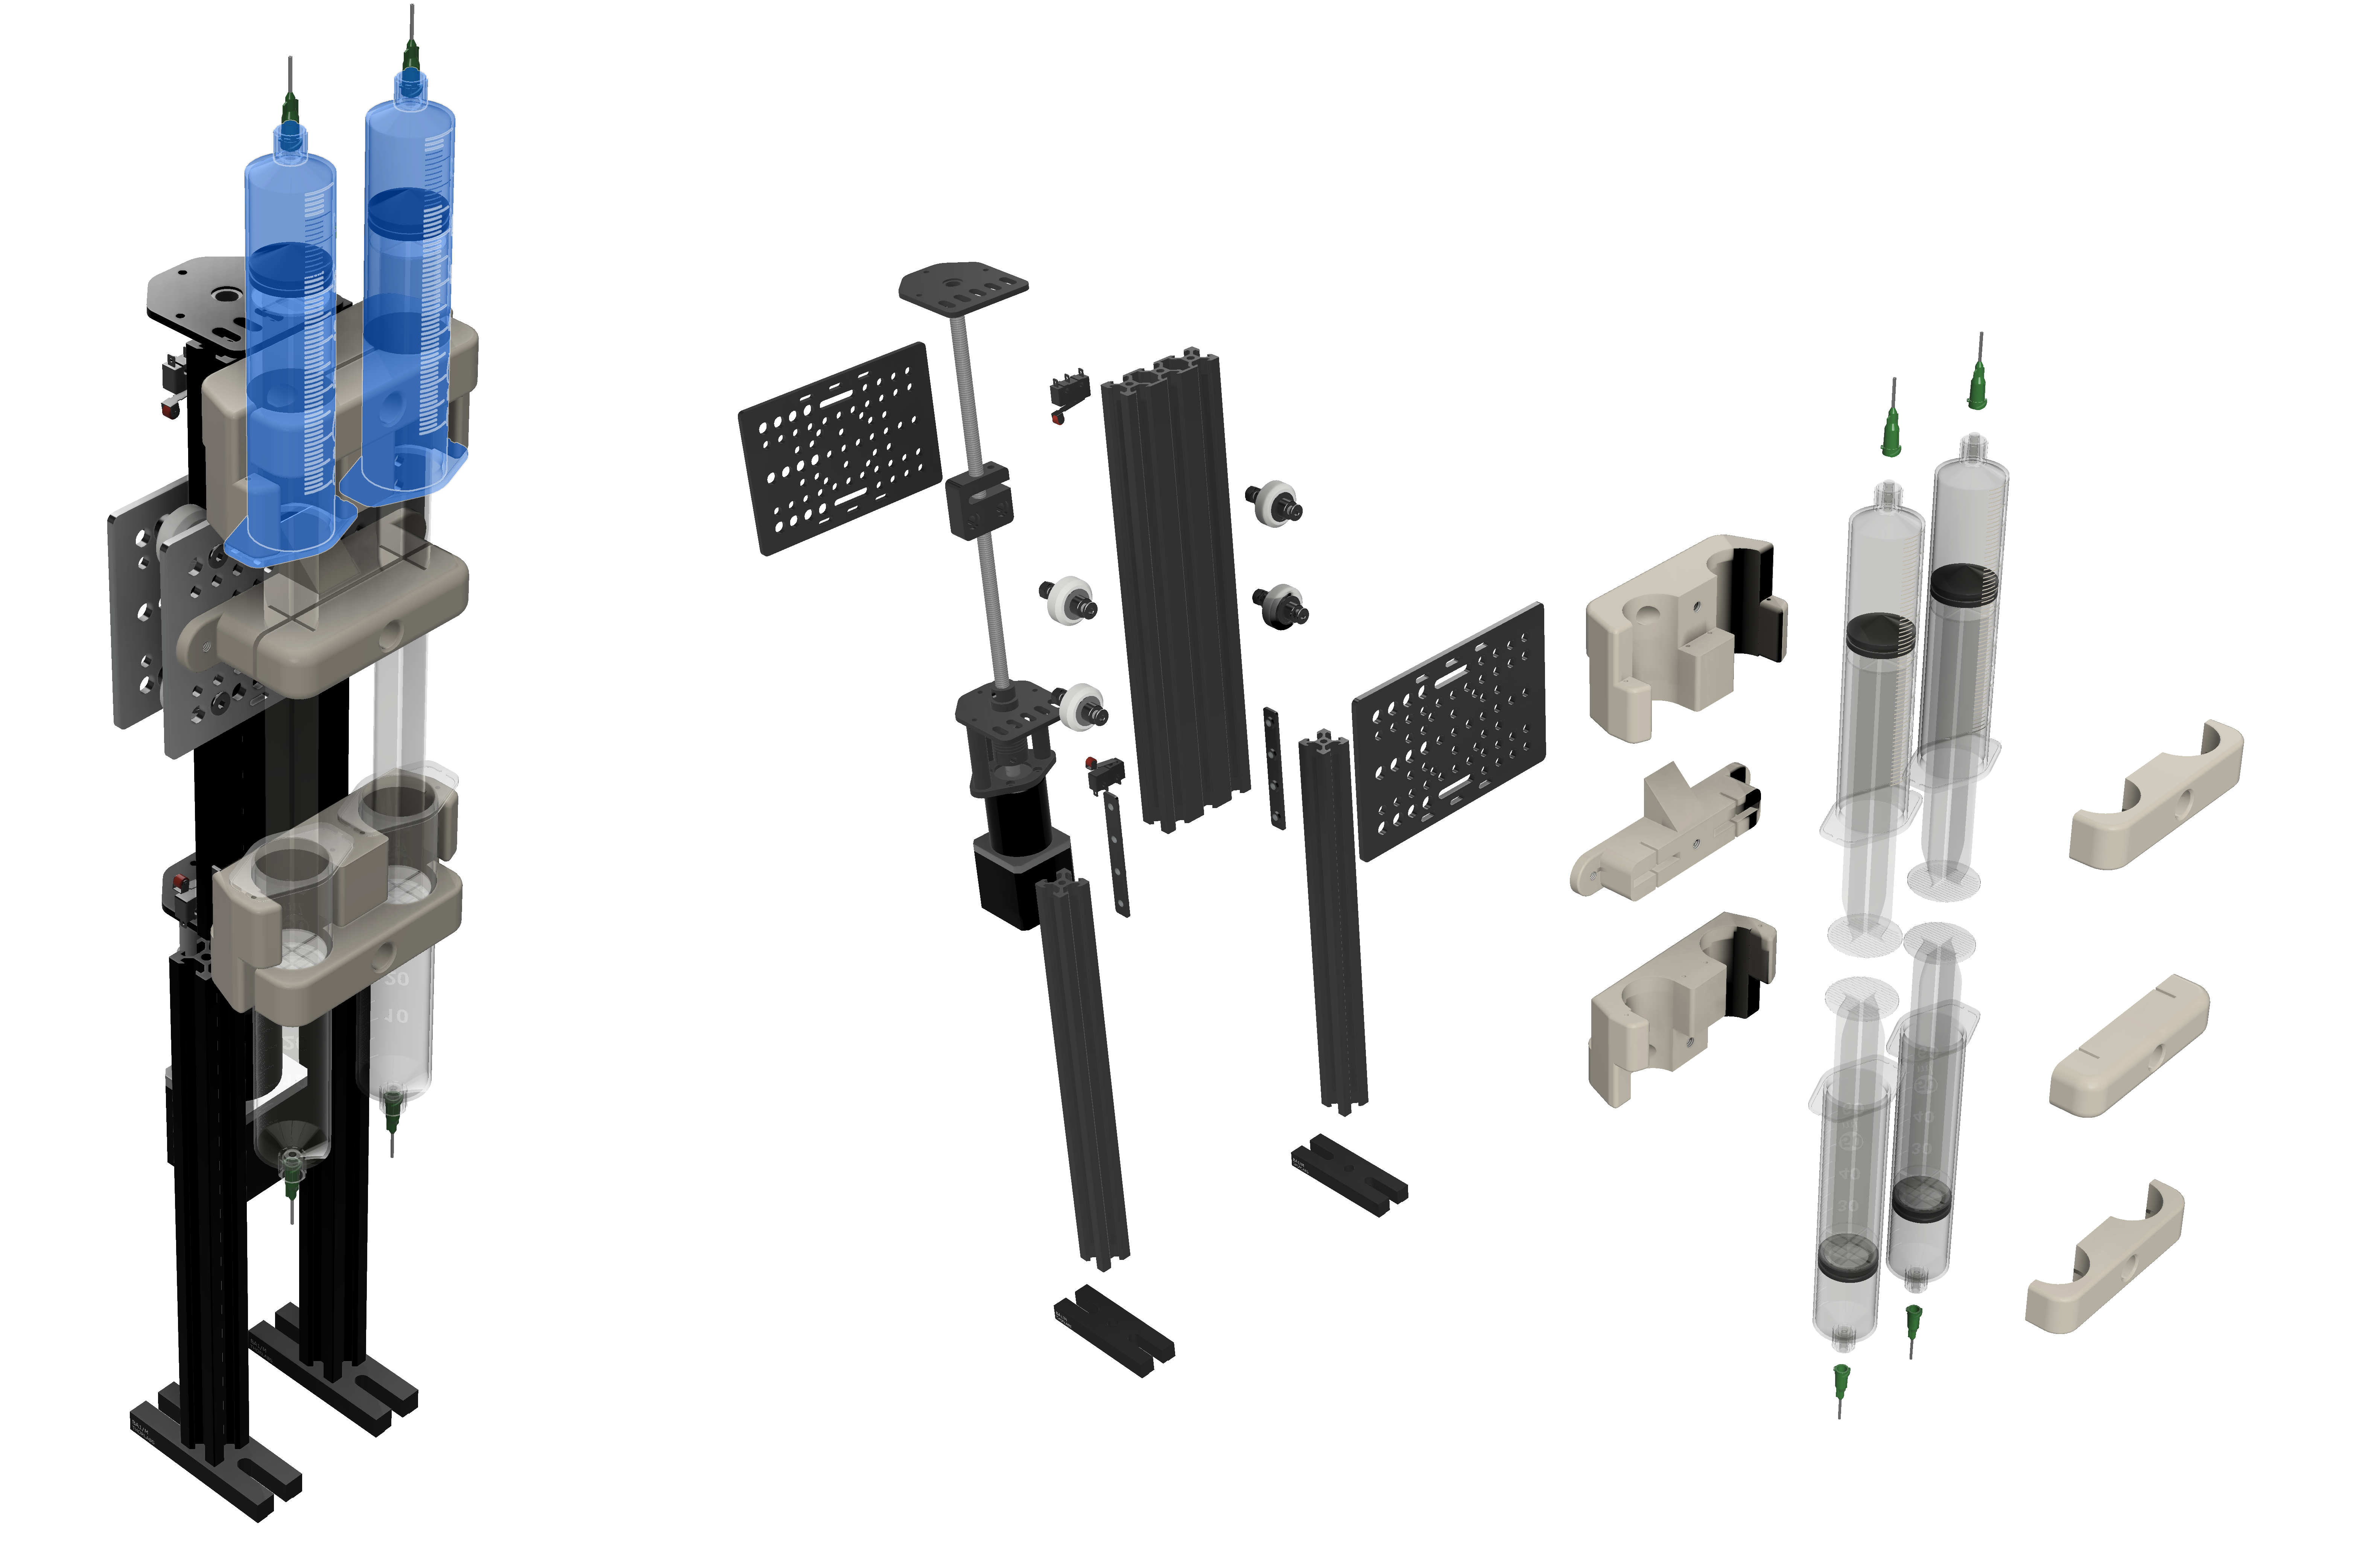
\includegraphics[width=0.95\textwidth]{part_2/assets/pull_push.png}
      \caption{\textbf{Dual mechanical structure} Dual custom pull-push syringe.}
      \label{dual_mechanical}
    \end{figure}

  It is crucial to isolate the animal from the exterior environment and of any light sources. A box that will contain the millifluidic chip and lighting system is constructed using MakerBeam rails and medium-density fibreboard sheets. A PMMA infrared transparent sheet is placed on the removable top panel to record the experiment while blocking visible light. The box contains, see Figure~\ref{dual_box}, two LEDs for visible and infrared light, a diffuser for homogeneous lighting, and a support to fix the millifluidic chip.

    \begin{figure}[h!]
      \centering
      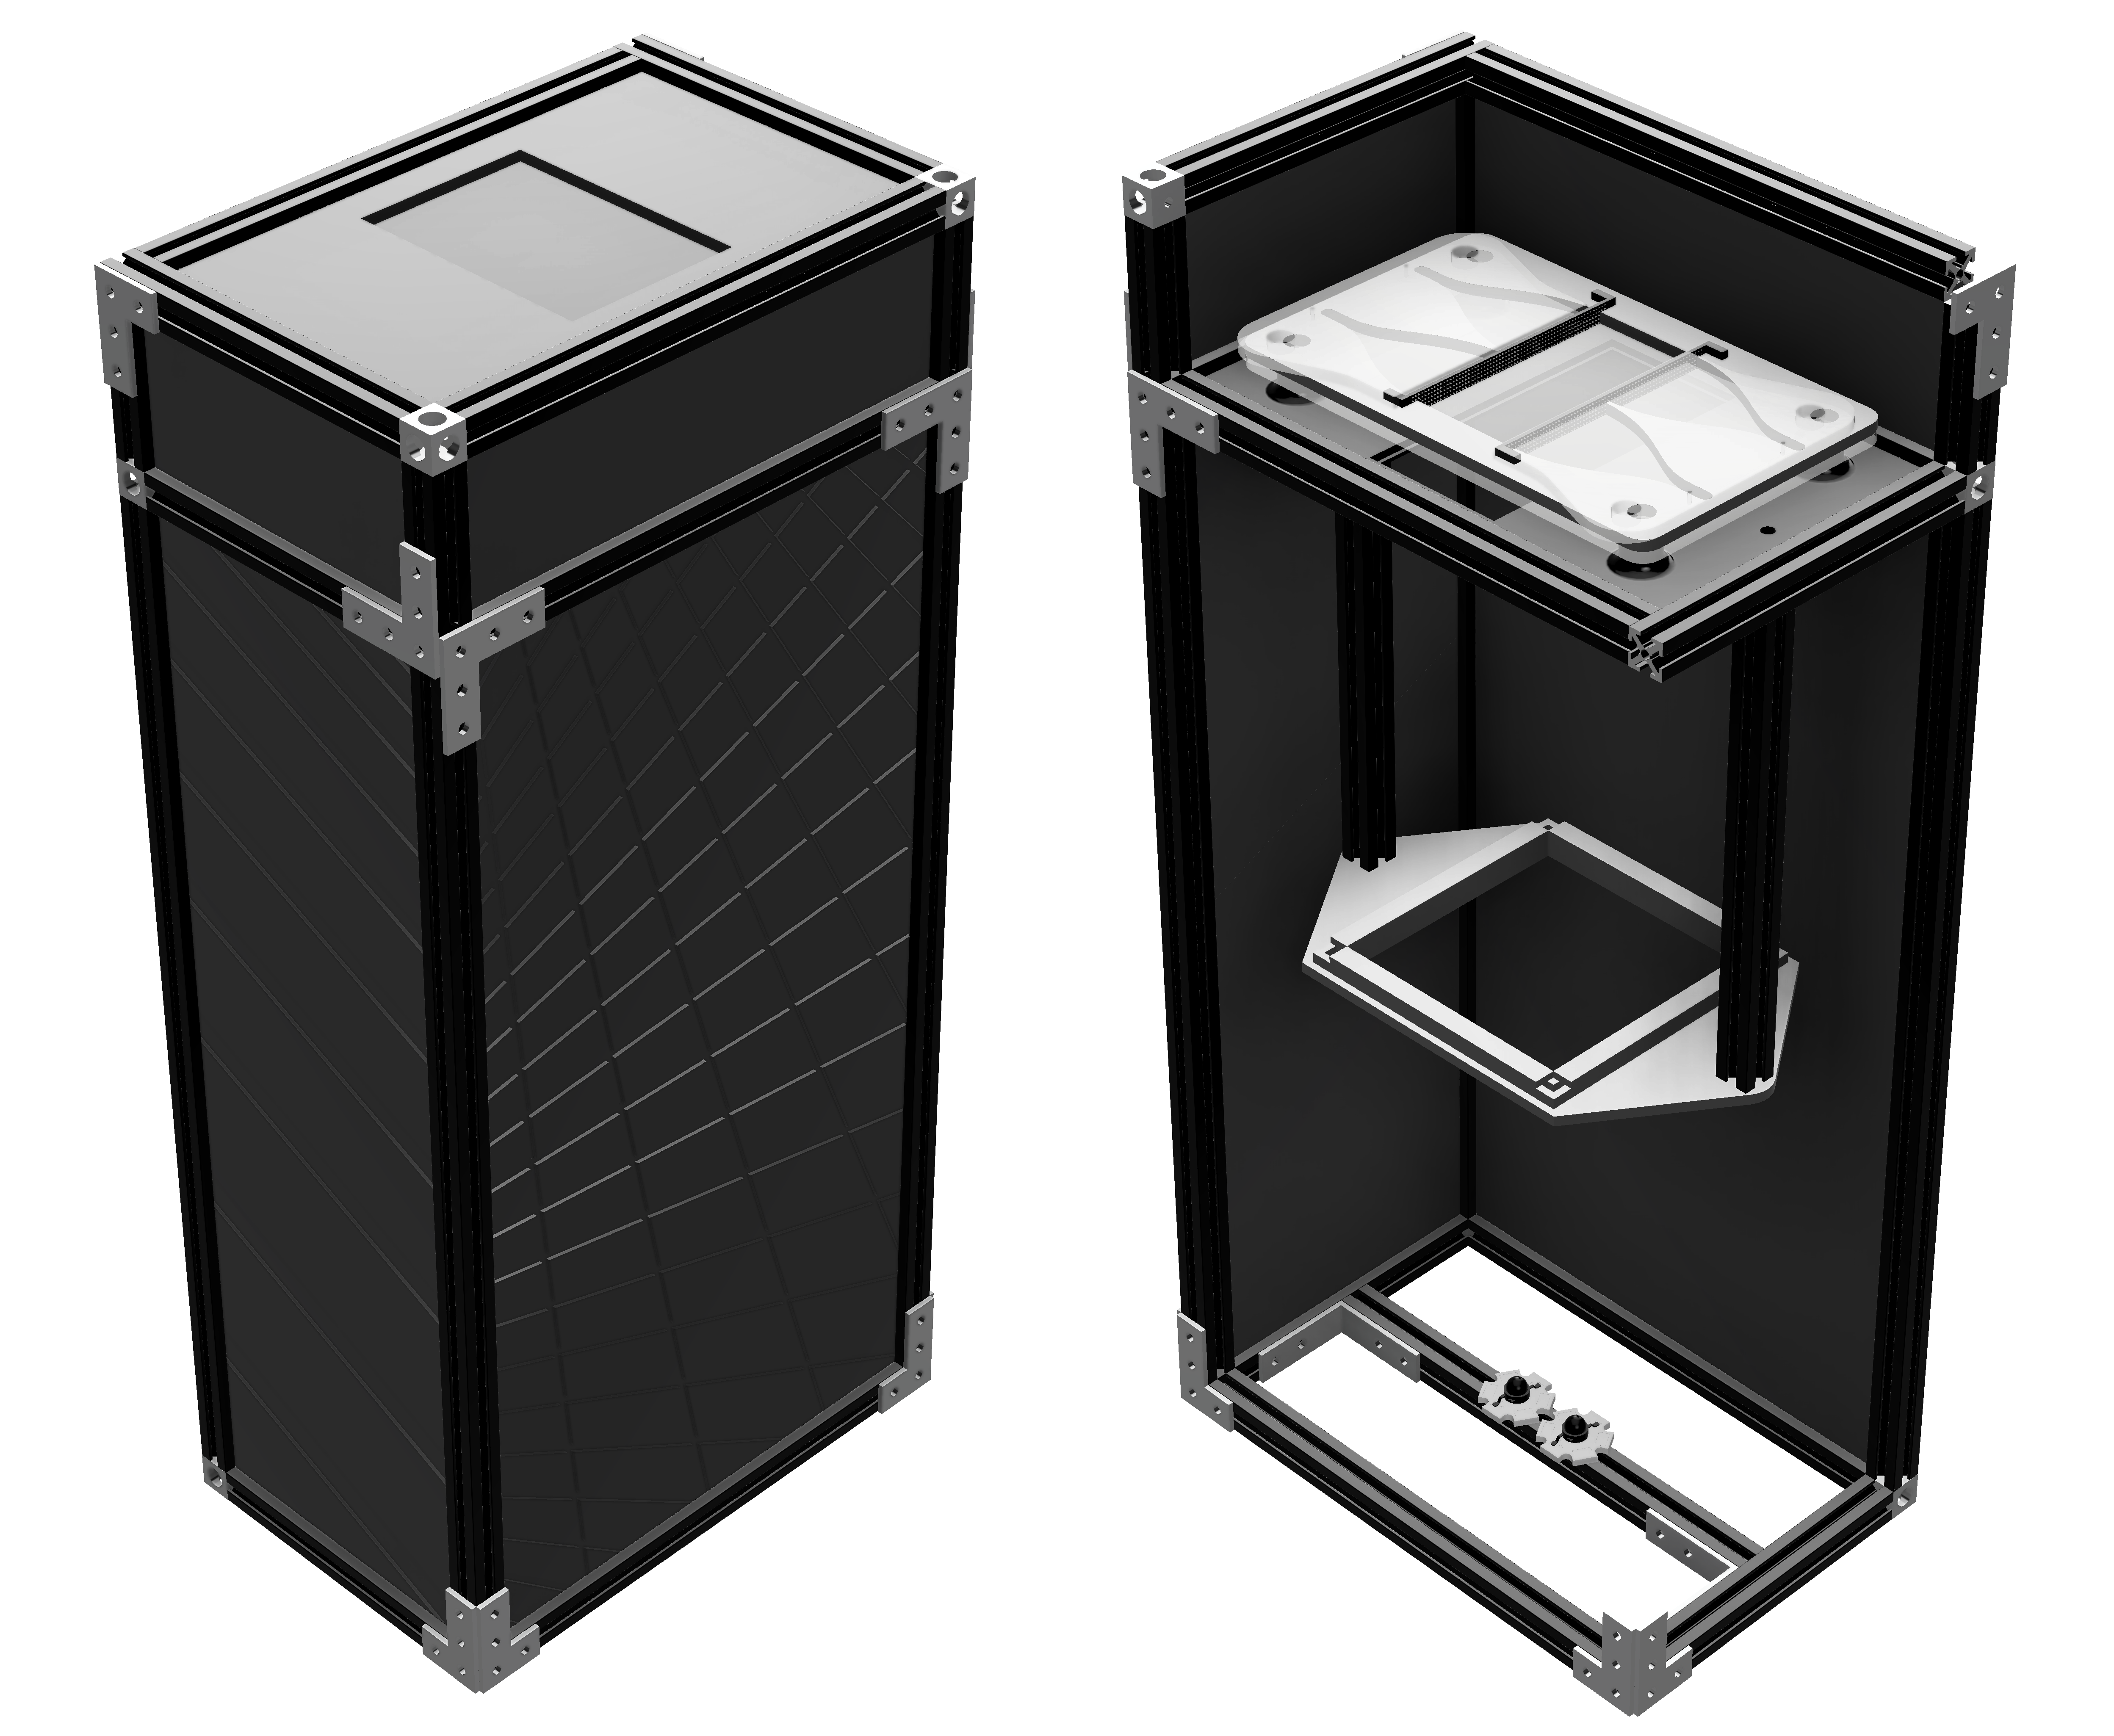
\includegraphics[width=0.75\textwidth]{part_2/assets/box.png}
      \caption{\textbf{Box} Dual box that will isolate the animal from the exterior.}
      \label{dual_box}
    \end{figure}

  A structure to maintain the camera on top of the box and secure the Raspberry and the power alimentation is built using OpenBuilds rails. It is best to build Dual on top of an optical breadboard to facilitate fixation and enhanced stability. All these elements need to be fixed firmly and leveled to avoid any bias that could disturb the animal during the experiment.

  \subsubsection{Millifluidic}
  The millifluidic chip that serves as a tank for the fish, see Figure~\ref{dual_chip_visu} is laser cutted in PMMA plastic that is transparent and presents excellent optic properties. The different parts are bonded using acetic acid \cite{}. The fish is restrained in the center by 3D printed and micro-machined nets, and profiled inputs and outputs allow a laminar flow.

    \begin{figure}[h!]
      \centering
      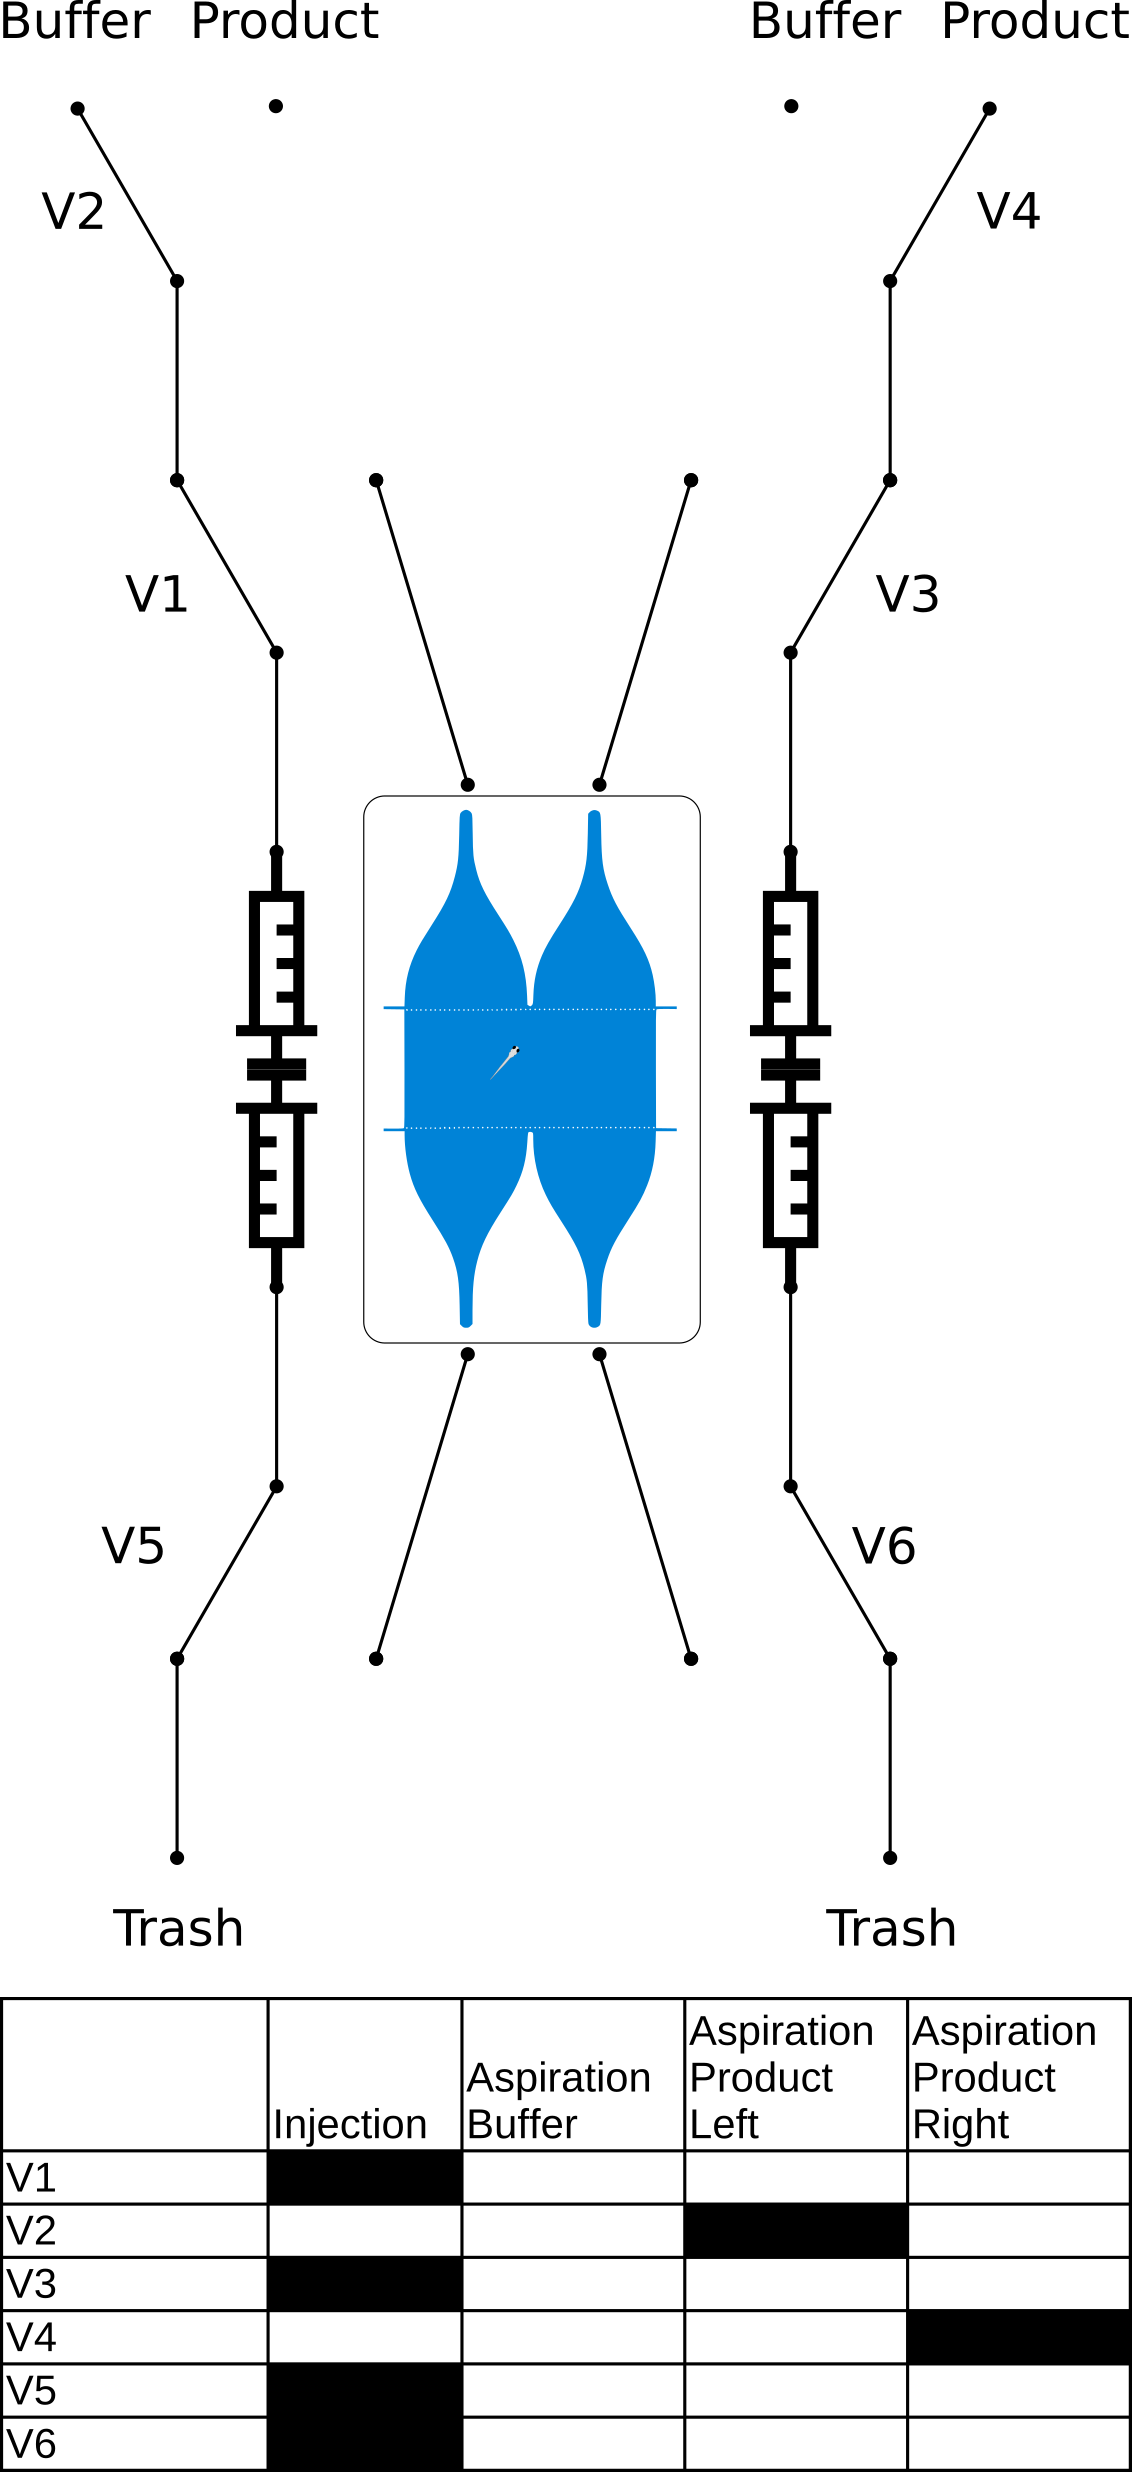
\includegraphics[width=0.50\textwidth]{part_2/assets/valve_schematic.png}
      \caption{\textbf{Valves manifold}}
      \label{valves_schematic}
    \end{figure}

  Sixty-milliliters syringes are fixed with 3D printed fixations on the actuator and connected with 2.2 mm diameters tubing to the microvalves circuit. Six three-ports microvalves are connected and form a circuit that allows performing cycles of filling and injection, see Figure~\ref{valves_schematic}.

    \begin{figure}[h!]
      \centering
      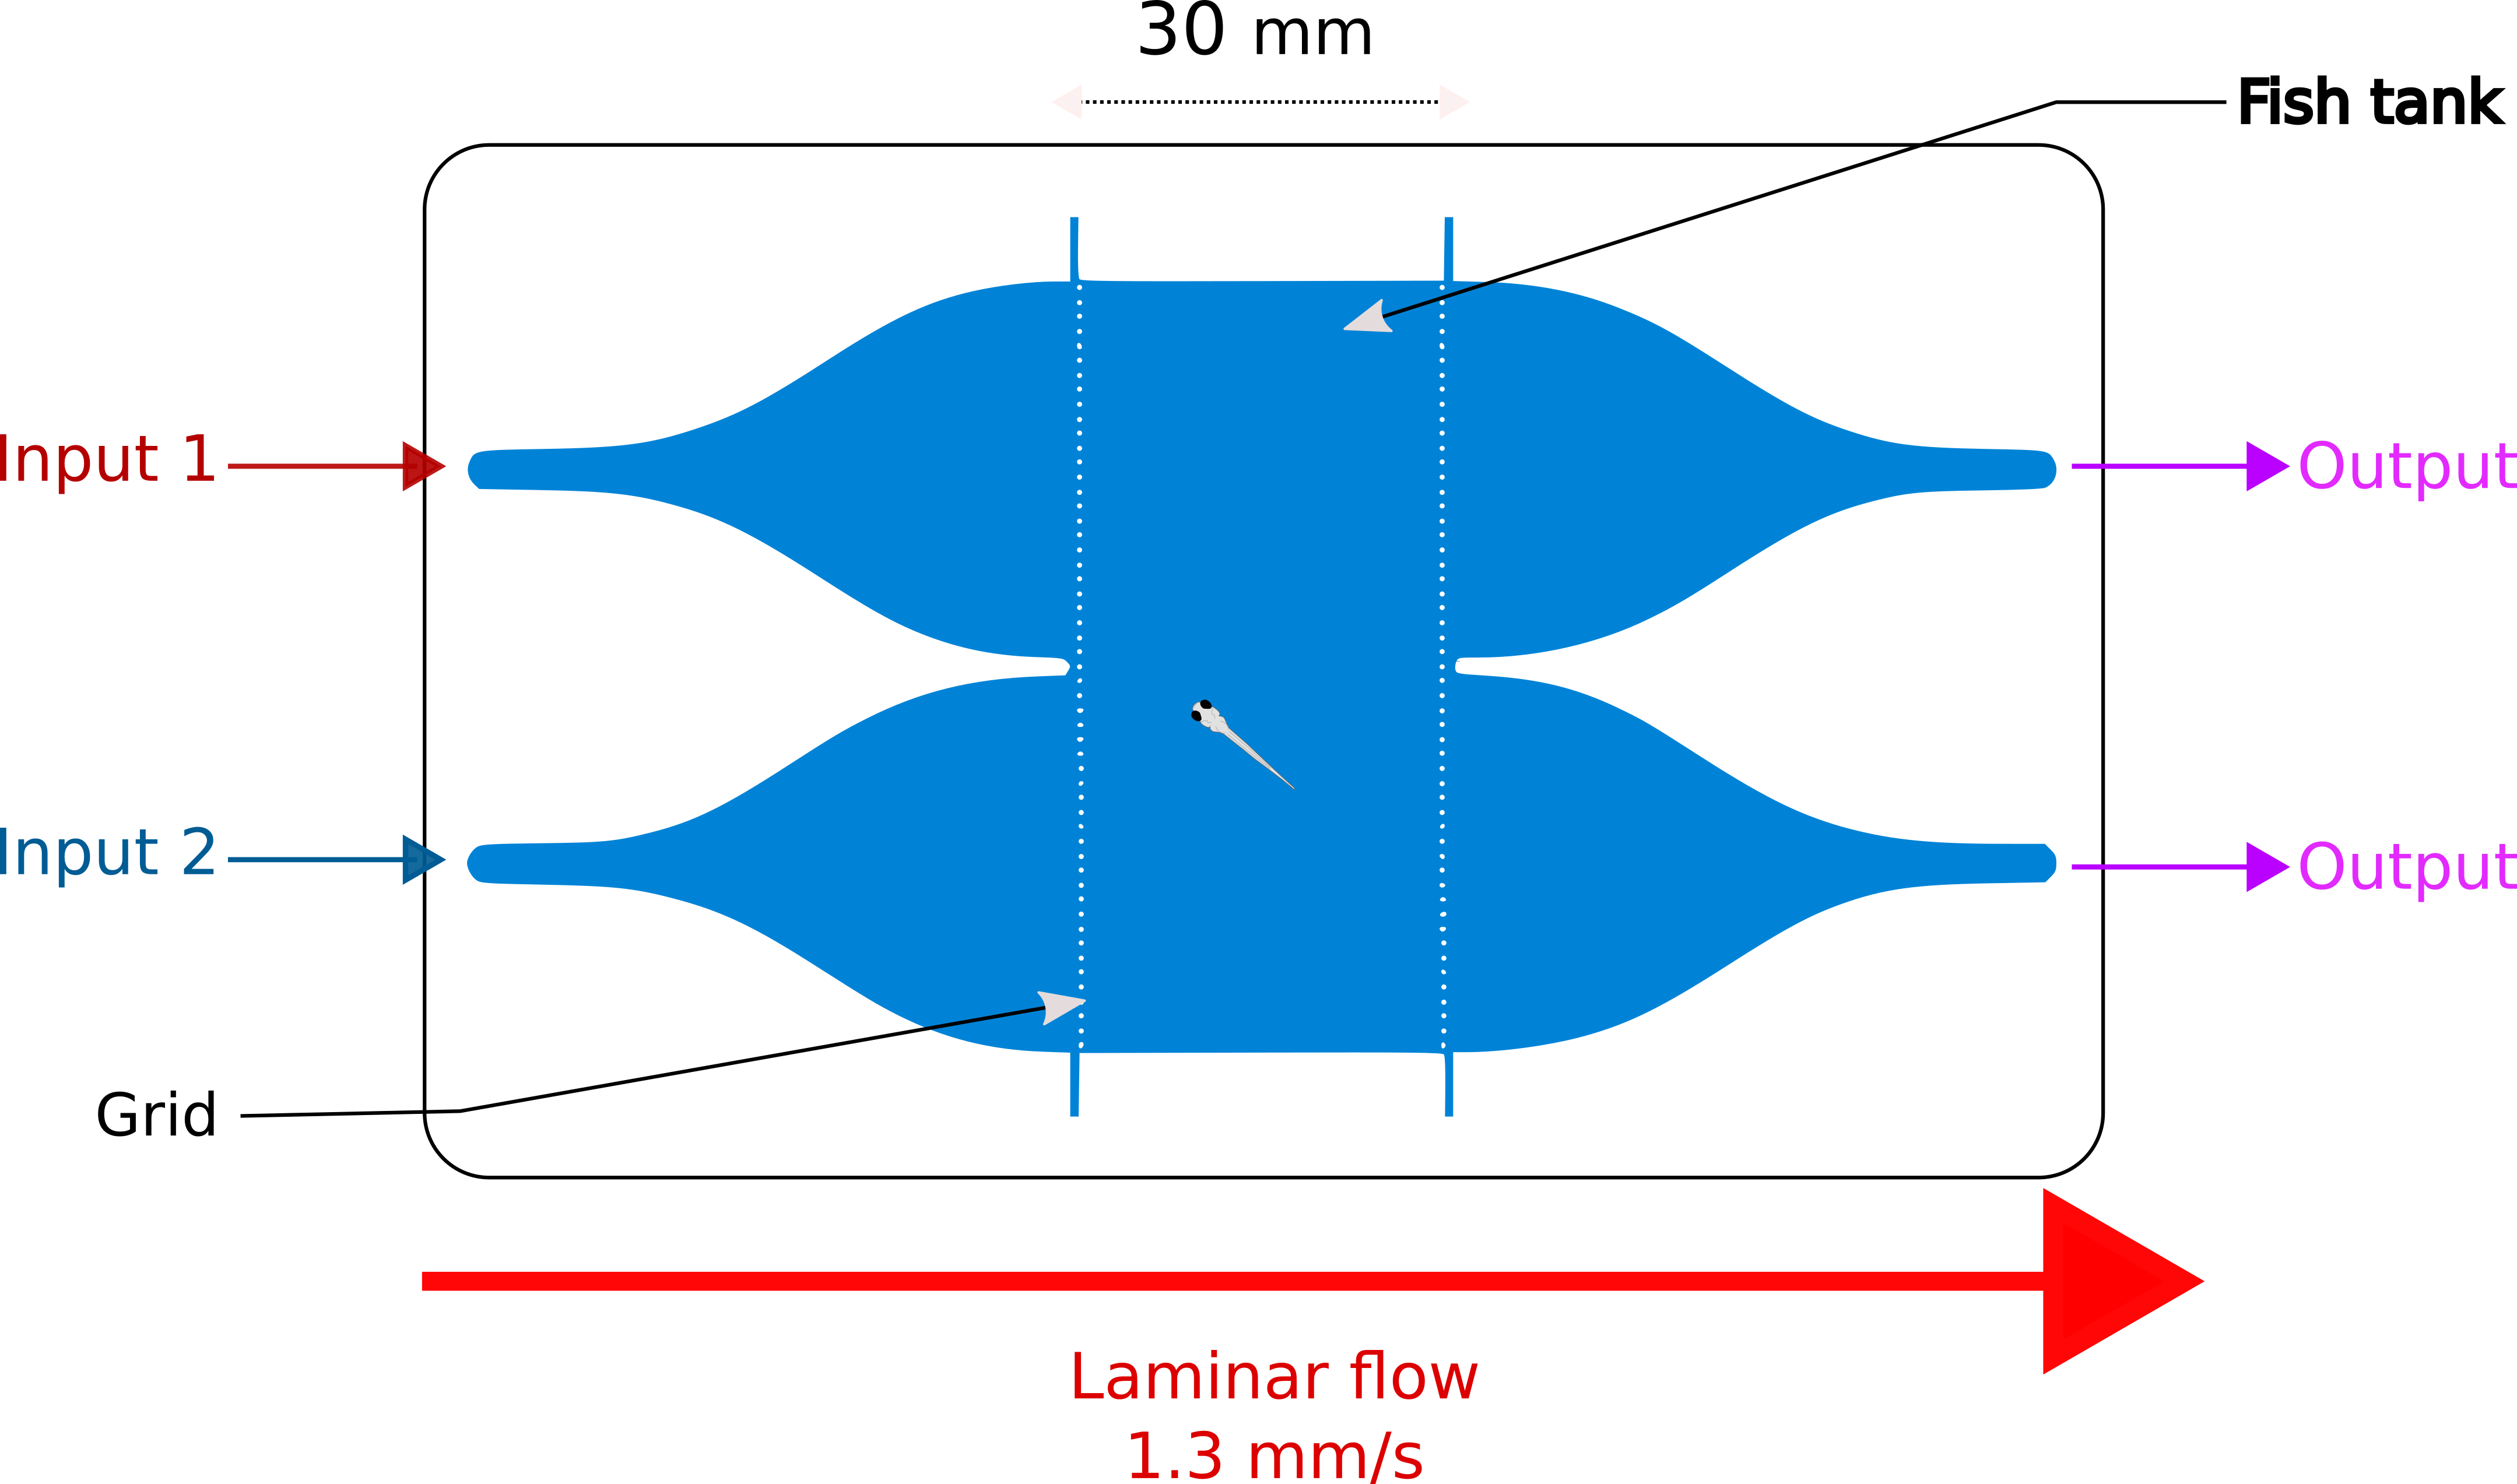
\includegraphics[width=0.75\textwidth]{part_2/assets/chip.png}
      \caption{\textbf{Millifluidic chip schematic.}}
      \label{dual_chip}
    \end{figure}

    \begin{figure}[h!]
      \centering
      \includegraphics[width=0.75\textwidth]{part_2/assets/chipxcf.png}
      \caption{\textbf{Millifluidic chip exploded view.}}
      \label{dual_chip_visu}
    \end{figure}

  \subsubsection{Imaging}
  The setup is lightened by transmission using an infrared LED placed at the bottom of the box. Homogenous lighting is obtained by placing a diffusor (tracing papers or white plastic sheet) at the box's mid-height. Experiments are recorded with a Chameleon 3 camera mounted with a 23-25 mm EFL lens connected directly to the computer via USB3. A PMMA infrared transparent sheet is placed between the camera and the lens to block visible light and only retrieve Dual's infrared lightening.

  \subsubsection{Electronic}
  The electronic system links the analogic mechanical and millifluidic system to the software. A custom printed circuit board (PCB) has been designed for Dual TODO(ajouter blueprint). It contains an Arduino Nano microcontroller; six half H-bridge controlling the microvalves based on the logic signals of the Arduino; a Big EasyDriver stepper motor controller to control the motor speed from a logic output of the Arduino; a potentiometer to control the intensity of the LED lighting. All the electronics and the syringe pump motor are powered by a 550W ATX computer power supply connected to the PCB.

  \subsubsection{Software}
  A software has been specifically developed to control the setup. The graphical user interface is developed using Qt, and the camera is interfaced to the software using the FLIR Systems SDK provided with the camera. The electronic system is controlled through the Arduino Nano flashed with a custom sketch and communicating to the software via USB serial. The software allows manual control of each system element, such as the microvalves, the camera, and the motor. It is possible (and advisable) to create custom experimental protocols, a simple text file, containing the necessary instructions to automate the filling and aspiration cycles to build experiments.

  Two versions of the software are available, one running on a modern desktop computer that can drive four Dual, another running on a Raspberry Pi4 that drives only one Dual. The latest solution offers better scalability since each Dual is independent. A custom version of Ubuntu 20.04 is preinstalled with the camera's SDK and the software. It can be downloaded at \url{https://github.com/LJPZebra/dual_control/releases} and flashed on an SD card or USB device. It is designed to work with a 7-inch touchscreen display allowing a compact and easy-to-use control.

  \subsection{Construction and usage}
  For our needs, we have built four Duals that we ran in parallel. The construction requires a laser cutting machine, a 3D printer, and workshop tools. It took about two weeks to build the four devices. The construction does not require any specific knowledge, and access to a FabLab is sufficient to carry out this project and find the required tools and help in the event of difficulties.

  In practice, using Dual is effortless. Once the experiment template is created, the only manual task remaining is to place the fish in the millifluidic chip, close the device, and play the experiment template. It is also necessary to check that the suction containers neither run out of water or chemical. It is then possible to do experiments with minimal manual interventions.

  A recurring problem we have encountered is the fouling of the millifluidic system. The dye used to visualize the flow ends up clogging the valves and tubes and can stop the system in the middle of an experiment. This problem can be solved by taking preventive habits. After each day of experiments, the millifluidic system has to be flushed with water. It can be performed automatically using an experimental template designed to wash all the microvalves thoughtfully. Microvalves can regularly be passed in an ultrasonic bath to clean them. The tubes have to be changed when worn out, which can append after several weeks of intensive usage. Another encountered problem was the syringe plunger wear. After several months of usage, the plunger's latex cap loses water-tightness, and the plunger has to be replaced, which can be done very quickly in less than 2 minutes.

  In this project, we did not use all the Dual potential. This setup can be adapted to other animals like \textit{Xenopus tropicalis} larvae, adults Danionella. It can serve to assess other preferences, notably the preference to light (phototaxis) with the integrated visible LED.

  \section{The Tropical River}
  Studying chemical perception and chemically-driven navigation in a turbulent aquatic environment like the one fish encounters naturally requires an experimental device capable of creating controlled flows and chemical jets. We have created an experimental device capable of delivering a temperature-controlled laminar flow while recording the fish in both visible and infrared light. An injection nozzle is used to create turbulent or laminar jets within this laminar flow.

    \begin{figure}[h!]
      \centering
      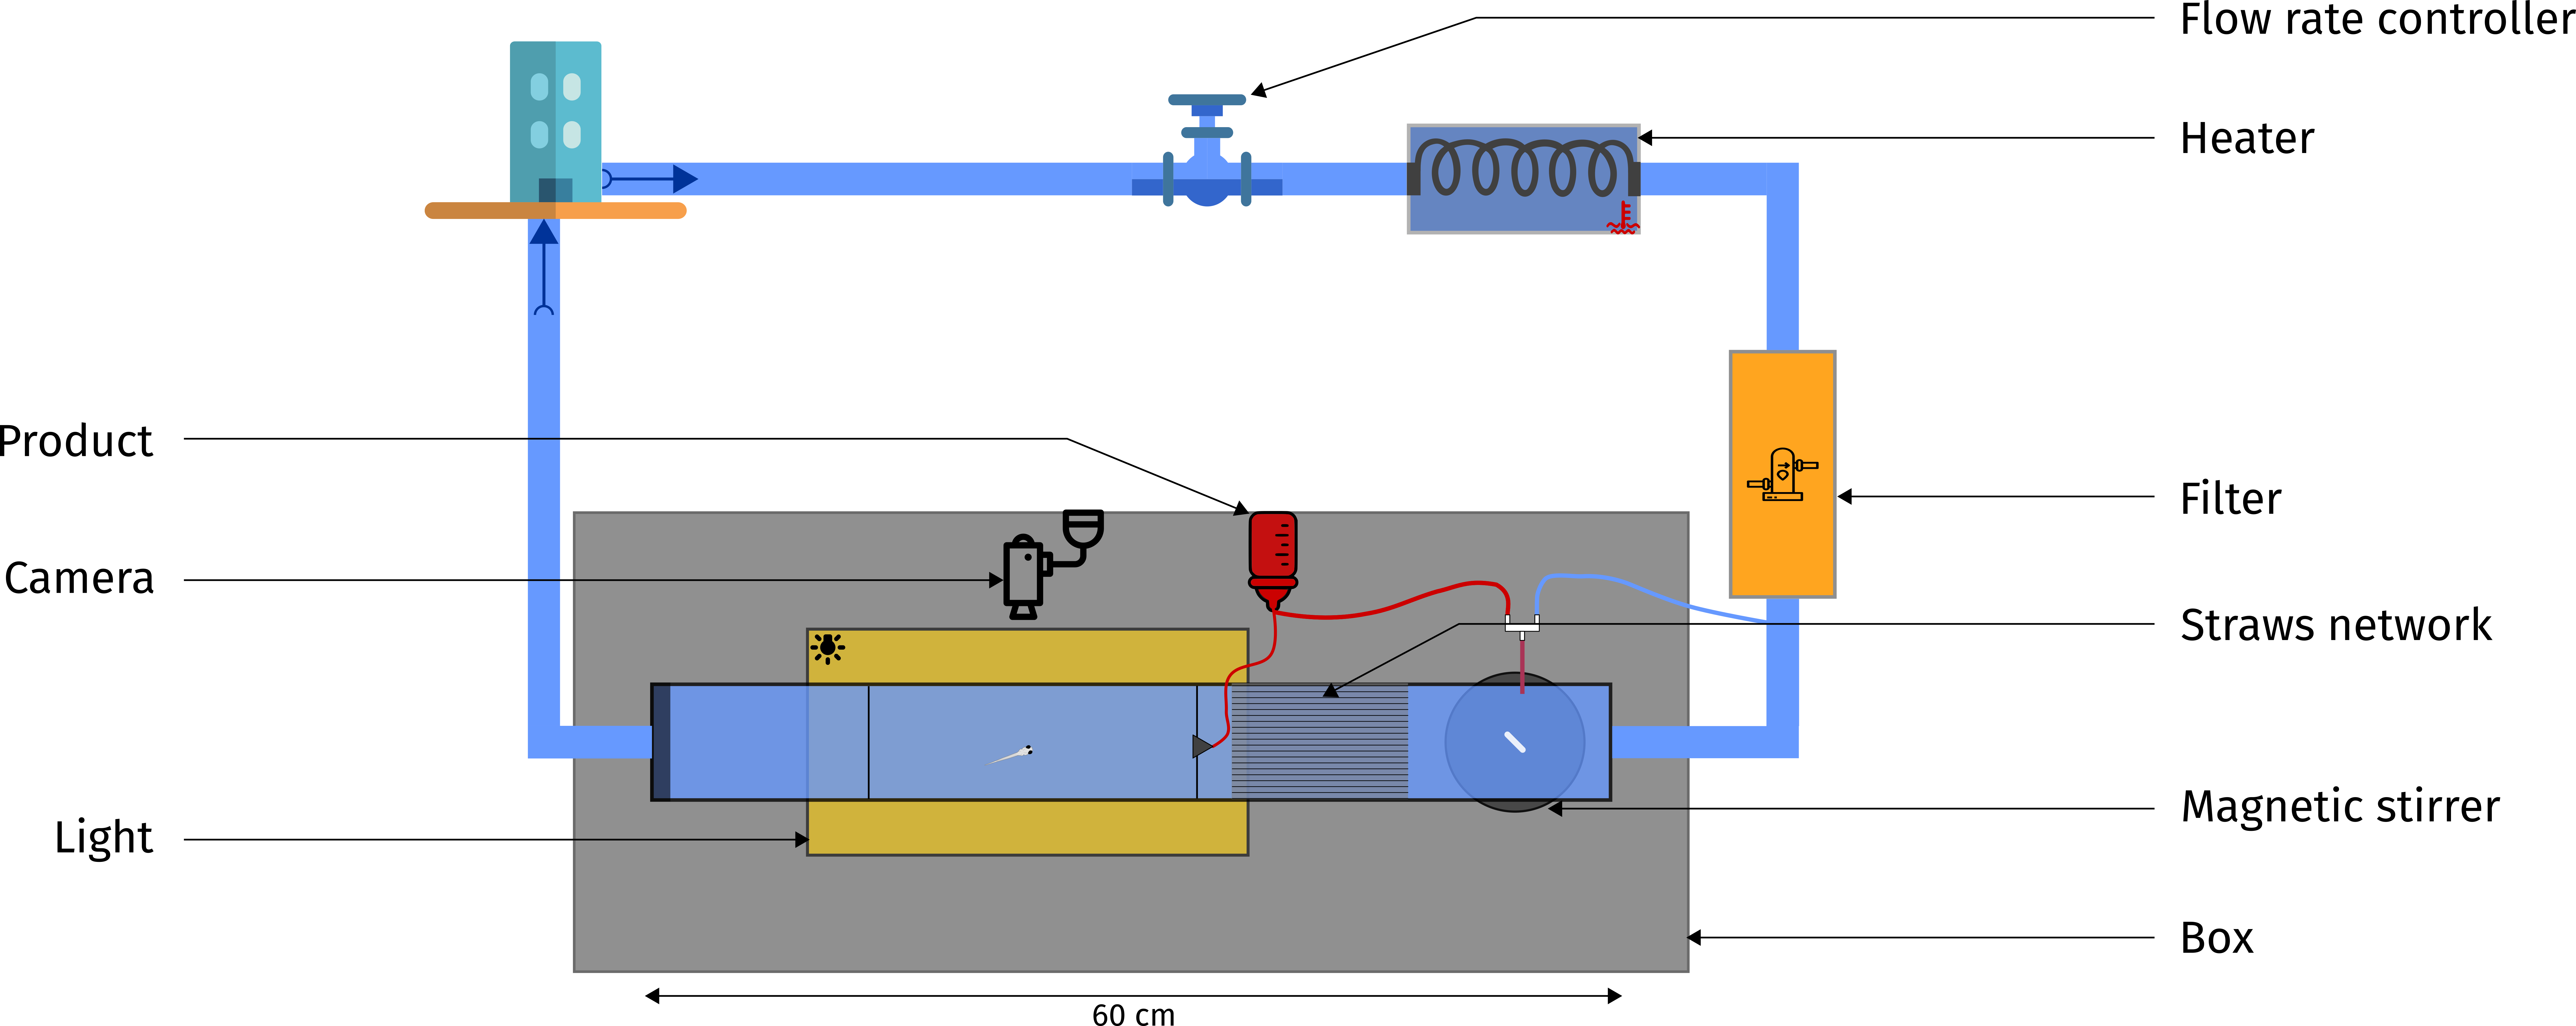
\includegraphics[width=1\textwidth]{part_2/assets/river.png}
      \caption{\textbf{The Tropical River} Schematic of the experimental setup.}
      \label{river}
    \end{figure}

\subsection{Description}
  \subsubsection{Structure}
  The device's structure consists of a channel assembled from transparent polycarbonate sheets machined precisely by the mechanical workshop and fixed with Norcan rails to form a channel (60x10x10 cm), see Figure~\ref{river}. A LED panel is placed under the channel to illuminate the setup by transmission in visible light. The setup can be illuminated from above by a ring of infrared LEDs or by transmission by covering the LED panel with a PMMA infrared transparent sheet. A Chameleon 3 camera with a TODO lens is placed above the channel to record the experiments and connected to the computer via USB3. A mirror is placed at 45 degrees of inclination from the horizontal on the channel's side to control the fish's vertical position. The whole channel is set inside a box constructed with Norcan rails and plywood sheets to isolate the fish from the surrounding environment.

  \subsubsection{Hydrodynamic}
  The canal is supplied at one end with water from the building's water system. Before entering the canal, tap water is filtered by an activated carbon filter and heated by a water bath. A network of straws is placed in the channel to obtain a laminar flow, and a solenoid valve can adjust the flow rate. The other end of the channel is left free. The outgoing water is redirected to the building's wastewater network because the products tested do not require any special treatment before being disposed of. The water height inside the channel can be controlled by modulating the dyke height placed at the end of the channel.

  It is possible to dilute a product inside the channel by using an injection nozzle located directly at the water supply outlet. A magnetic stirrer is placed inside the channel, before the straws network, to facilitate dilution. Another injection nozzle can be placed inside the channel, after the straws network, to create a turbulent or laminar jet. It is supplied by an external tank, and the flow rate can be adjusted by gravity and delivery automatically controlled by a valve system.

  \subsubsection{Software}
  The control software allows to retrieve and control all the variables of the experiment. By default, it allows selecting the flow rate, temperature, injection valves, and camera settings. A vital function of the software is the ability to build experimental protocols. Easy to build, the protocol template is a simple text file specifying for a given device a variable's desired value at a given time point. Any Arduino sensor or control device that follows a convention detailed in \url{https://github.com/LJPZebra/the_tropical_river_control} can be called in these protocols without the need to modify the software.

  \subsubsection{Camera}
  The camera's options are directly accessible inside the software using the Spinnaker SDK. Metadata like temperature, relative times to the experiment, flow rate, or user-specified value can be saved inside the image.

  \subsubsection{Temperature}
  The temperature regulation is made using a coiled heat exchanger tube added to the water inlet and immersed into a Neslab RTE water bath capable of cooling and warming. A temperature sensor is placed inside the channel and sends the instantaneous temperature to the control software. The software can control the water bath via an RS232 serial connector selecting the temperature using a PID feedback system. Despite large variations of the building's water temperature, this system allows a precise and rapid temperature regulation.

  \subsection{Usage and limitation}
  This experimental device is, in practice, very versatile. The ability to control the velocity and the temperature of the laminar flow, as well as the injection of products in an automated and quantified manner while recording the fish, allows the study of a wide variety of behaviors like rheotaxy, chemotaxis, and thermotaxis. The height of water in the channel can be modulated, making it possible to use adult and larval fish in the same setup.

  The insertion of chemical in the flow does not allow us to reuse the water. This is why the water supply is done using the water network of the building. Although filtered, the water quality depends on the building's water quality, which is usually not a problem for juvenile and adult fish that are reared in filtered tap water from 2 weeks onwards. However, this can be more problematic for larvae, which are more fragile and require calibrated water (E3). Although the experiment's duration is limited only by the computer's storage, small air bubbles appear in the channel after a few hours. This phenomenon is due to the dissolved gases present in the tap water and is detrimental to the fish. The activated carbon filter reduces this phenomenon, but it remains present and limits the maximum experimental time to a few hours.

\chapter{Results}
  \section{Methods}
  In the next sections, we will present the experimental protocol that we used and the analysis methods we developed to assess zebrafish chemical preference.

  \subsection{Experiment}
  \paragraph{Protocol} Fish chemical preference was assessed using Dual setup in a one-hour long experimental in a protocol detailed in Figure~\ref{exp_protocol}. This protocol is subdivided into 4 cycles of 15 minutes each:
\begin{itemize}
  \item B1: a cycle where buffer is injected on the two sides that serves as a control.
  \item P1: a cycle where a product is injected on one side and water on the other.
  \item B2: same cycle as B1 that will serve to flush the system of any residual product.
  \item P2: same as P1 but with sides inverted.
\end{itemize}

    \begin{figure}[h]
      \centering
      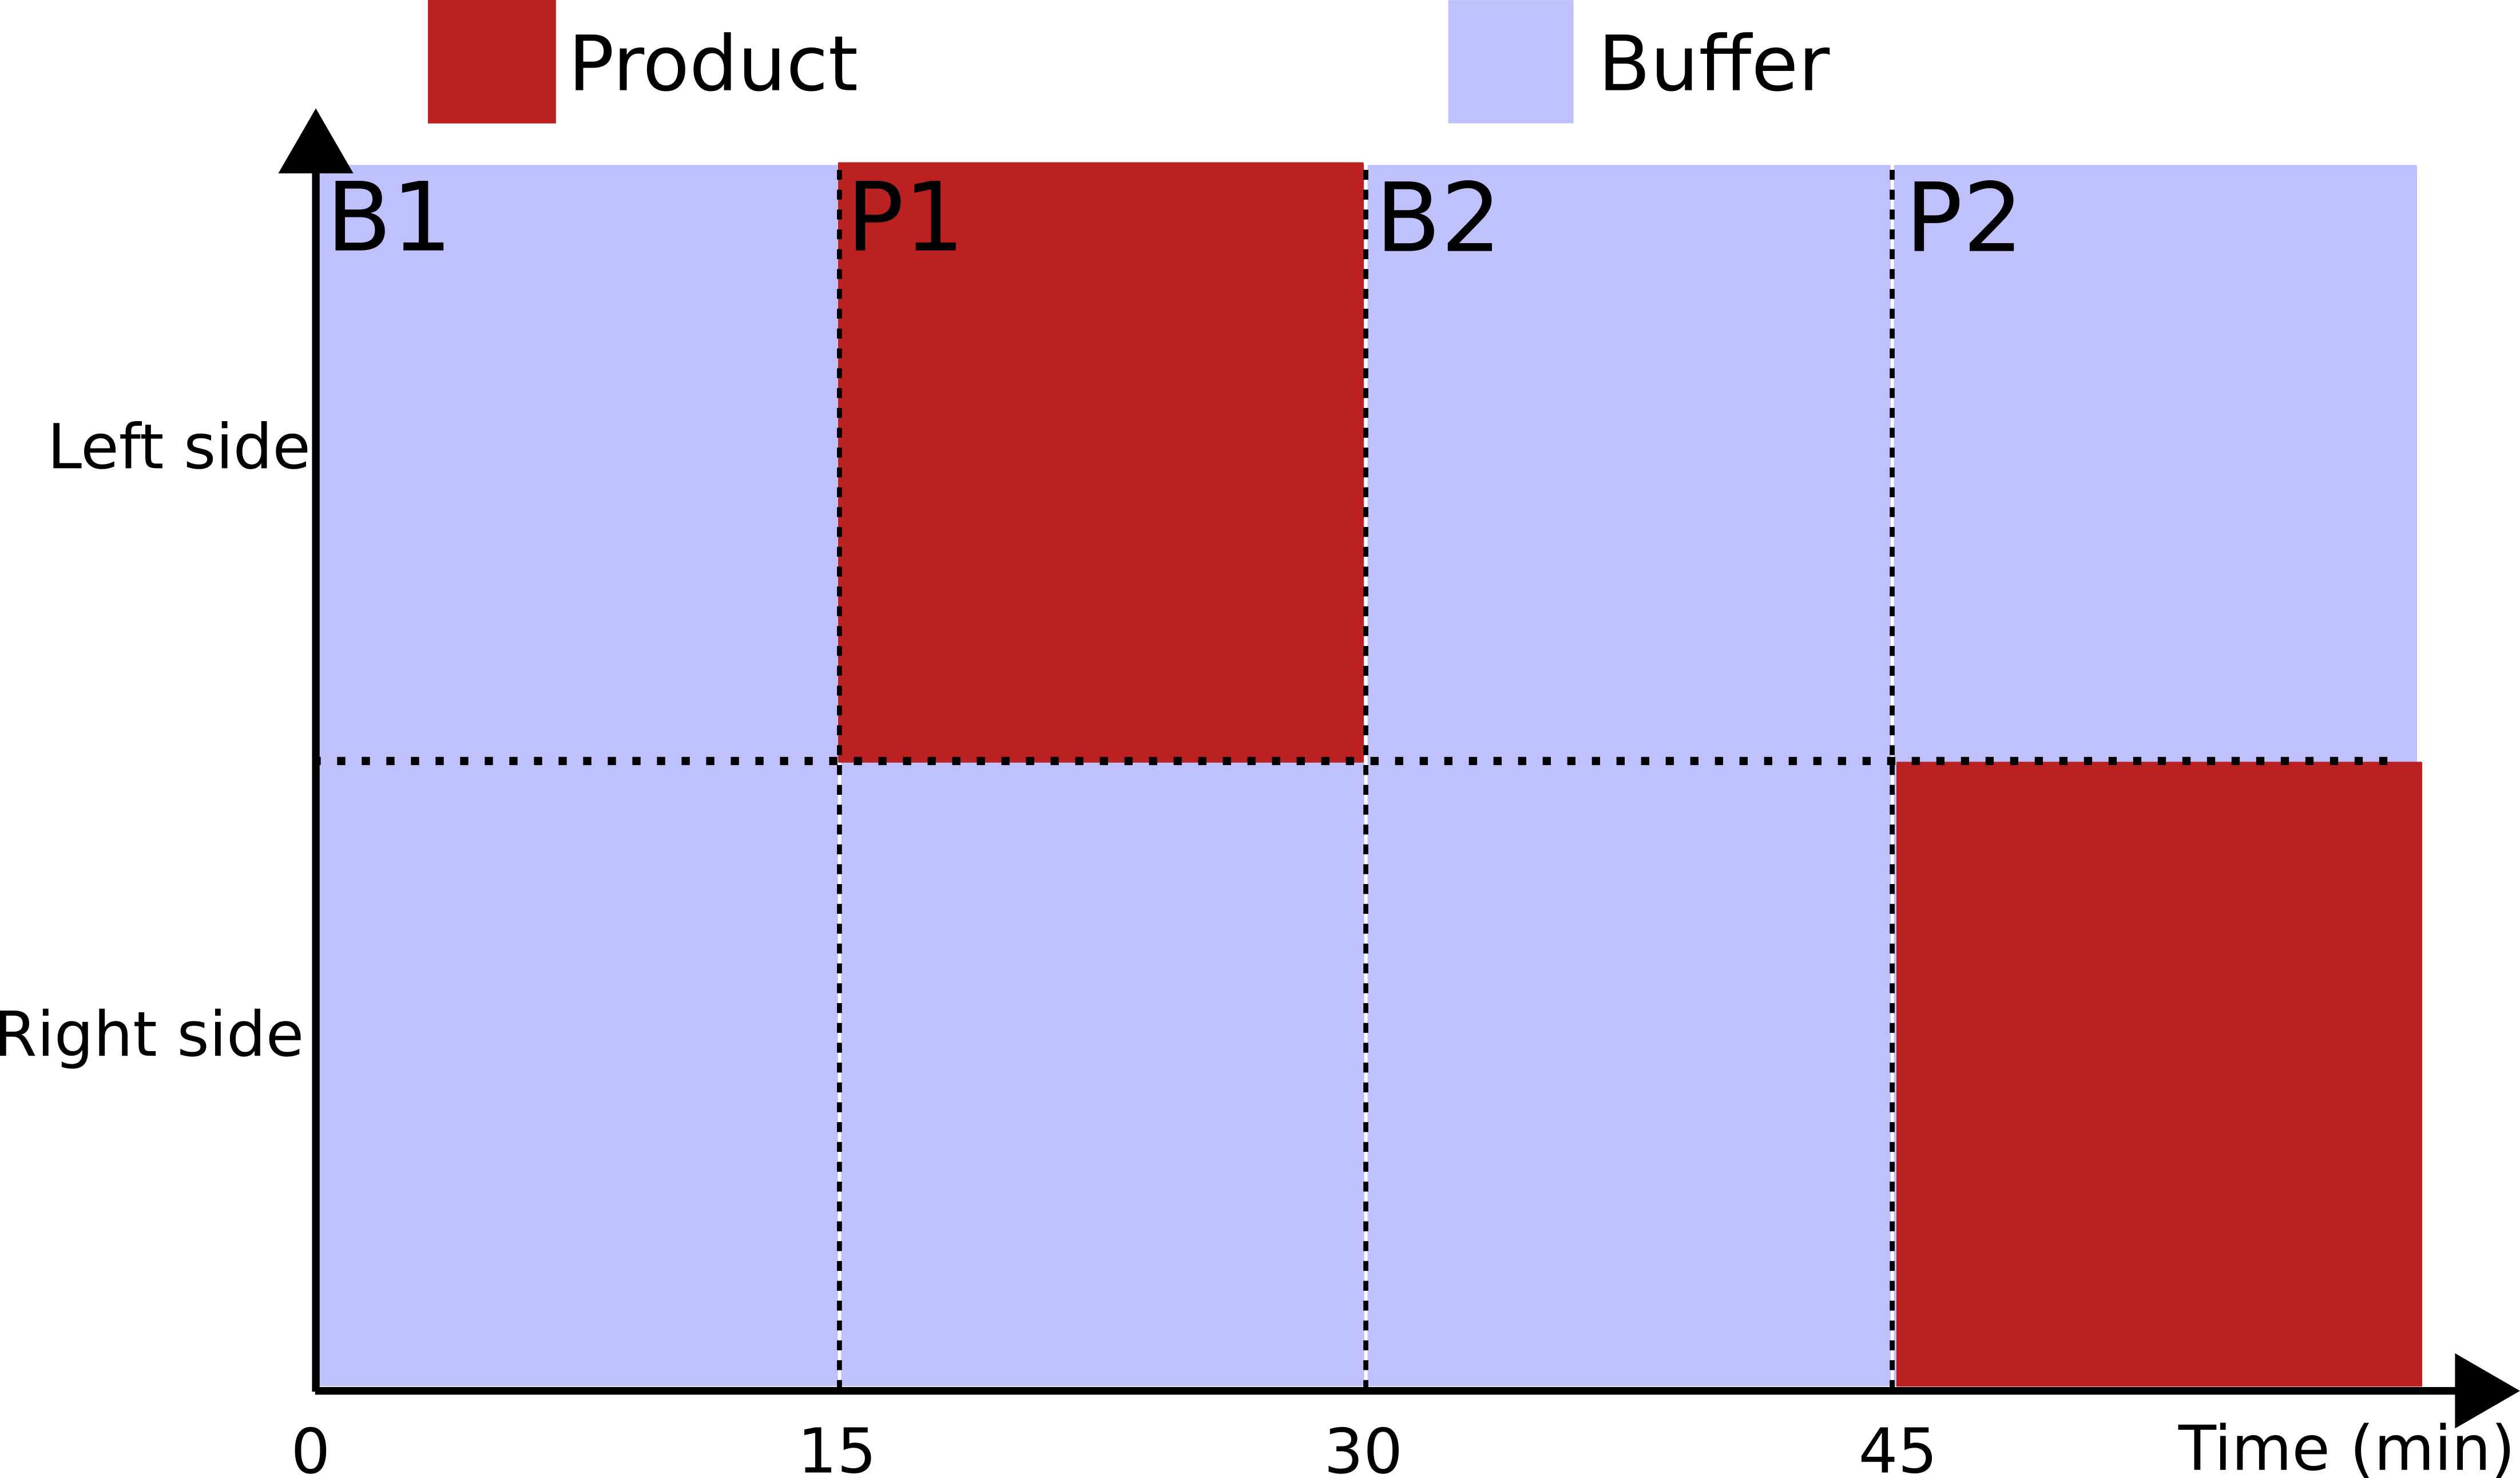
\includegraphics[width=0.75\textwidth]{part_2/assets/protocol.png}
      \caption{\textbf{Protocol} Experimental protocol used to assess zebrafish chemical preference. Product cycles P1 and P2 were regularly inverted to avoid any side bias.}
      \label{exp_protocol}
    \end{figure}

  \paragraph{Fish} In the following experiments, we use larval (6-8 days post-fertilization) and early juveniles (14 to 21 weeks post-fertilization) zebrafish. Preferences were assessed without changes in rearing condition before the experiment, except for ATP and adenosine, where fish were starved 24 hours before the experiment, a protocol inspired from \cite{wakisaka2017adenosine}. Chemicals were dissolved in a buffer the day of the experiment: E3 \cite{} for larvae and degassed tap water for juveniles.

  \paragraph{Flow visualization} All the experiments were performed in the dark to isolated chemical senses from other sensory inputs, in particular visual perception. The flow was visualized using an infrared dye, an emulsion of silicone oil, and infrared lightening. TODO(completer avec info Laeticia)

  \subsection{Analysis}
  The project's original idea was to use FastTrack \ref{part1} and an automatic custom-developed image analysis pipeline to monitor the fish and interface position. It would have made it possible to assess fish preference and decipher how the fish modulate its behavior when in contact with a chemical. However, in particular cases, the fish's complex behavior coupled with the challenge to get the interface position accurately pushed us to develop a manual method of analysis that we have used to characterize more precisely the fish behavior.

  \paragraph{Time-base preference index} The preference index is a measure of the attraction or repulsion of a product. It is defined from the times spent inside and outside the product as follows:
  $$
  PI=\frac{t_{product}-t_{buffer}}{t_{product}+t_{buffer}}
  $$
  \noindent When $PI=1$, the fish spend all its time on the product side; thus, the product is attractive. When $PI=-1$, it is the complete opposite, and the product is repulsive. $PI=0$ means that the fish spent the same amount of time on each side; thus, the product is neutral.

  The critical point of this analysis method is to define when the fish is in the product. A coarse-grained analysis would be to assimilate the interface with its median position. Most of the time, it is accurate and reflects the fish preference well. On the other hand, it will provide no insight at the crucial moment where fish take a decision, i.e., when the fish cross the interface. We try unsuccessfully to develop an automatic interface extraction using the difference in contrast between buffer and water. But, complex behaviors of the fish at the interface that were challenging to quantify automatically, the large amount of data, and time constraints pushed us to use a manual method of quantification.

    \begin{figure}[h]
      \centering
      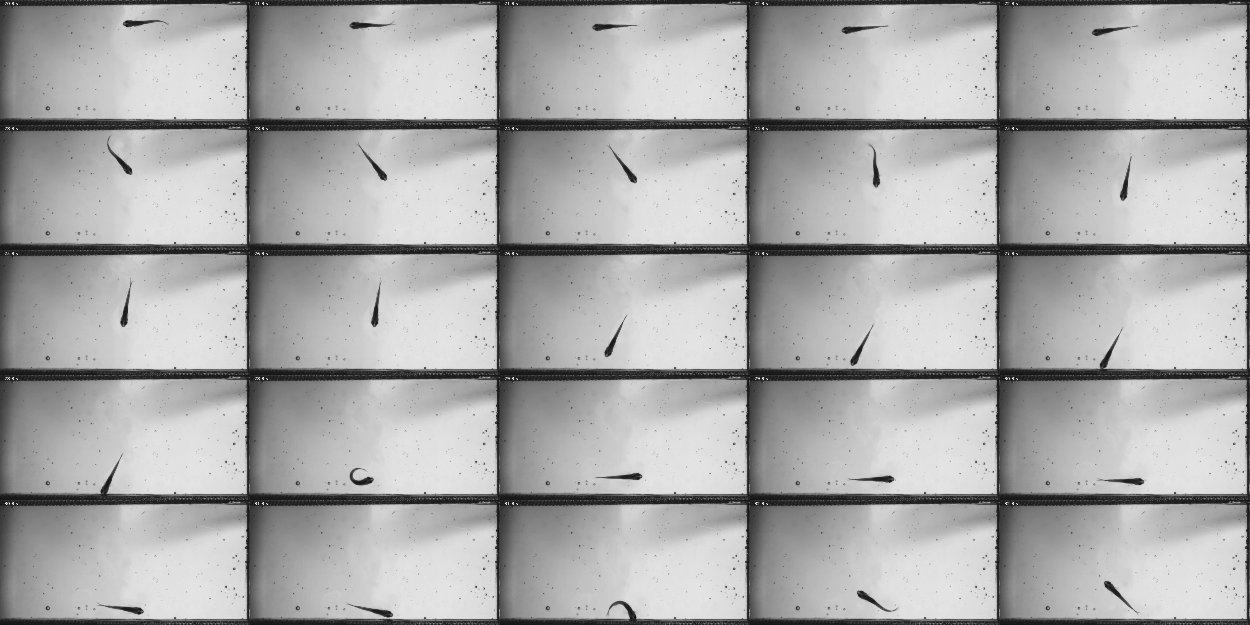
\includegraphics[width=0.75\textwidth]{part_2/assets/behavior.jpg}
      \caption{\textbf{Complexe} Example of a complex behavior where the fish swim inside the interface. The fish is creating advection and automatically extract the interface position is challenging.}
      \label{behavior_comp}
    \end{figure}

  \paragraph{Event analysis} To be time-efficient, we choose to develop a manual analysis method. We choose 4 characteristics and meaningful events, see Figure~\ref{events}, to quantify the behavior: when the fish cross the interface to change side (PB, BP) and when the fish sense the interface and return to the side where it was (BB, PP). By recording these events, we can quantify the moment where the fish make a decision, which was not possible with the time-based analysis.

    \begin{figure}[h]
      \centering
      \includegraphics[width=0.75\textwidth]{part_2/assets/events.png}
      \caption{\textbf{Events} The event-based method of quantification distinguish 4 types of events that can occurs during P1 and P2 product cycles.}
      \label{events}
    \end{figure}

  To count these events, we performed a blind analysis where movies were anonymized and scrambled. The events counting was performed by two independents individuals and then pulled together to get the average and deanonymized.

  We look first at the correlation between the two independents analyses, see Figure~\ref{correlation_count}, to check for human bias. The correlation between each fish's events count was equal to $0.97$, indicating that there is no significant bias or disagreement between the analysis.

    \begin{figure}[h]
      \centering
      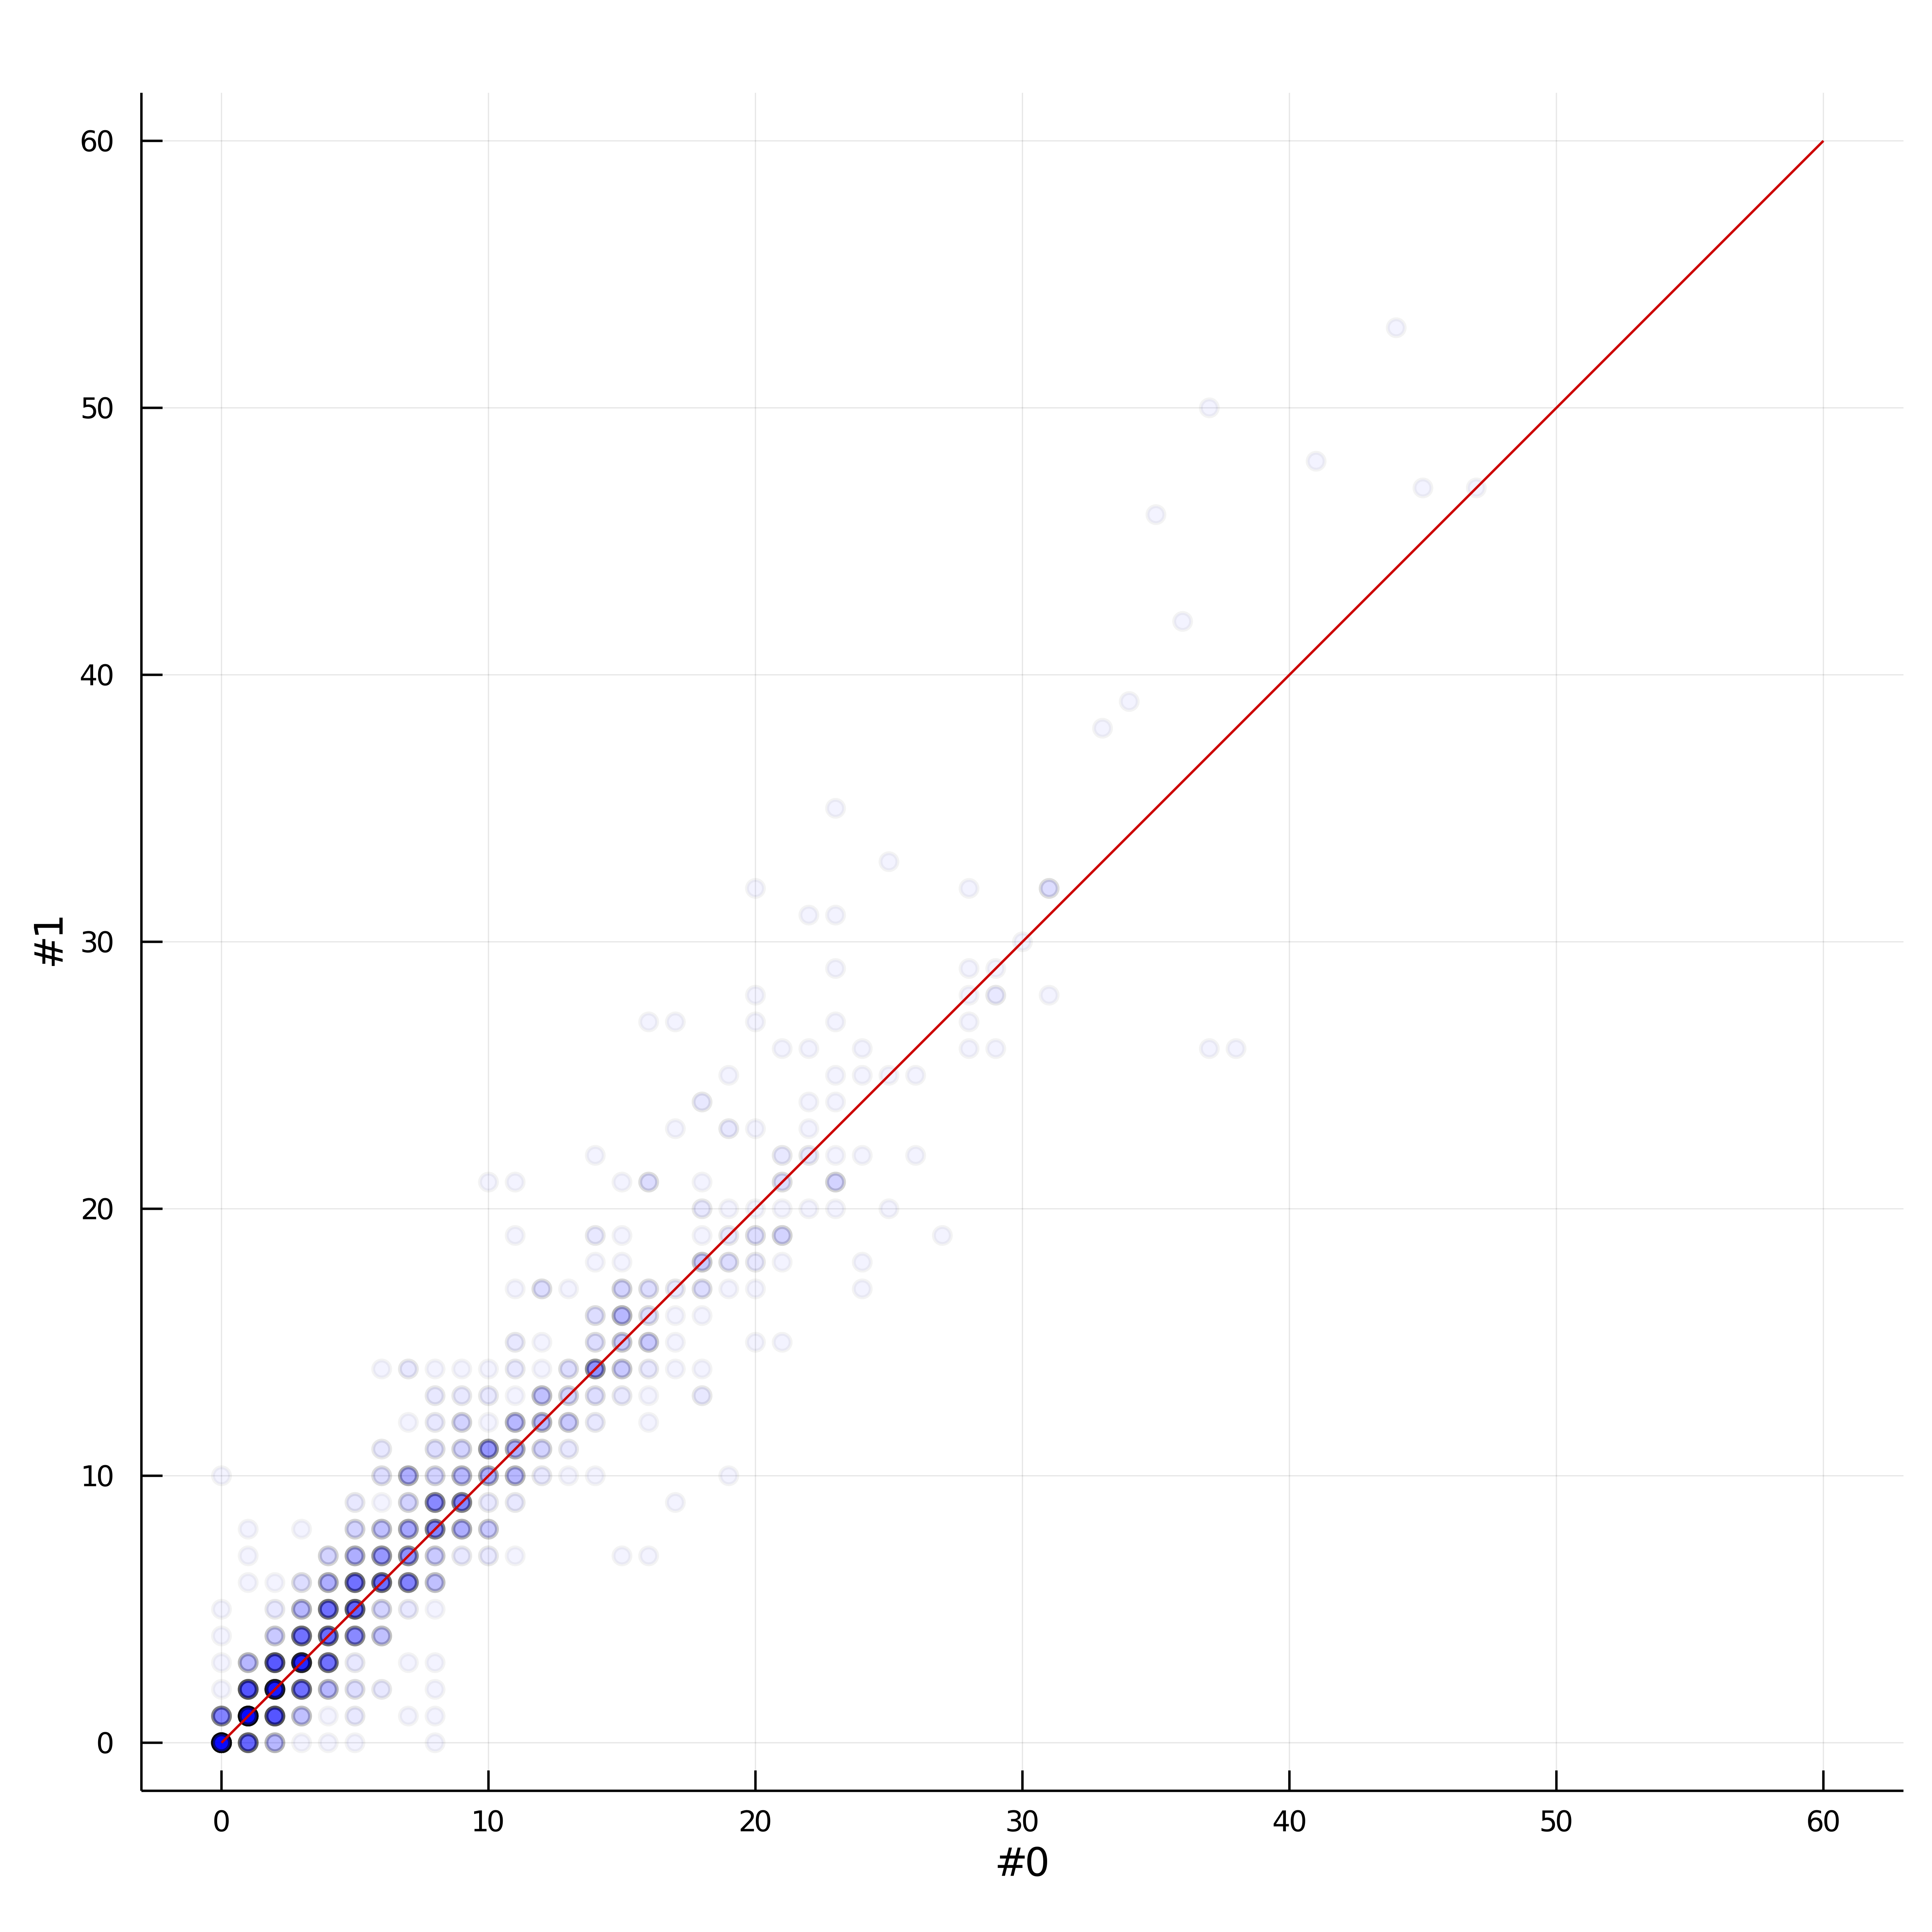
\includegraphics[width=0.50\textwidth]{part_2/assets/correlation.png}
      \caption{\textbf{Analysis correlation} Correlation between the two independent event-based analysis. One point is the count for one event type for one fish. Red line is the identity line. The point color intensity is encoding the number of points at the same coordinate.}
      \label{correlation_count}
    \end{figure}

  We can define an event-based preference index as follow:
  $$
  PI = \frac{n_{BP} + n_{PP} - n_{BB} - n_{PB}}{n_{BP} + n_{PP} + n_{BB} + n_{PB}}
  $$
  \noindent This preference index is slightly different from the time-based one. It will only consider fish decisions and not be impacted by the fish inactivity and freezing.

  \paragraph{Ratio exploration-exploitation} Besides the preference of the fish, an interesting quantity that we can look for is the type of behavior. We can distinguish two modes of behavior: an exploration mode where the fish cross the interface to explore the environment and an exploitation mode where the fish stay on the same side and make touch-and-turn at the interface. Note that this quantity is by any means a preference indicator.

  The ratio exploration-exploitation can be computed based on the event as follows:
  $$
  r=\frac{n_{BP} + n_{PB}}{n_{BB} + n_{PP}}
  $$
\noindent When $r=1$ there is as much exploration as exploitation, $r<1$ there is more exploitation and $r>1$ more exploration. In the event where $n_{BB} + n_{PP} = 0$ we take $r=0$ (pur exploration),  and $n_{BP} + n_{PB} = 0$ we take $r=\infty$ (pur exploitation).

  \paragraph{Model} Based on the events recordings, we can build a two-state Markov chain model (Figure~\ref{markov_model}). We can define the probability of transfer as follows:
  $$
  p = \frac{n_{BP}}{n_{BP} + n_{BB}}
  $$
  $$
  b = \frac{n_{PB}}{n_{PB} + n_{PP}}
  $$
  \noindent With $p$ the probability of going from the buffer to the product and $b$ the probability of going from the product to the buffer.

  \begin{figure}[h]
    \centering
    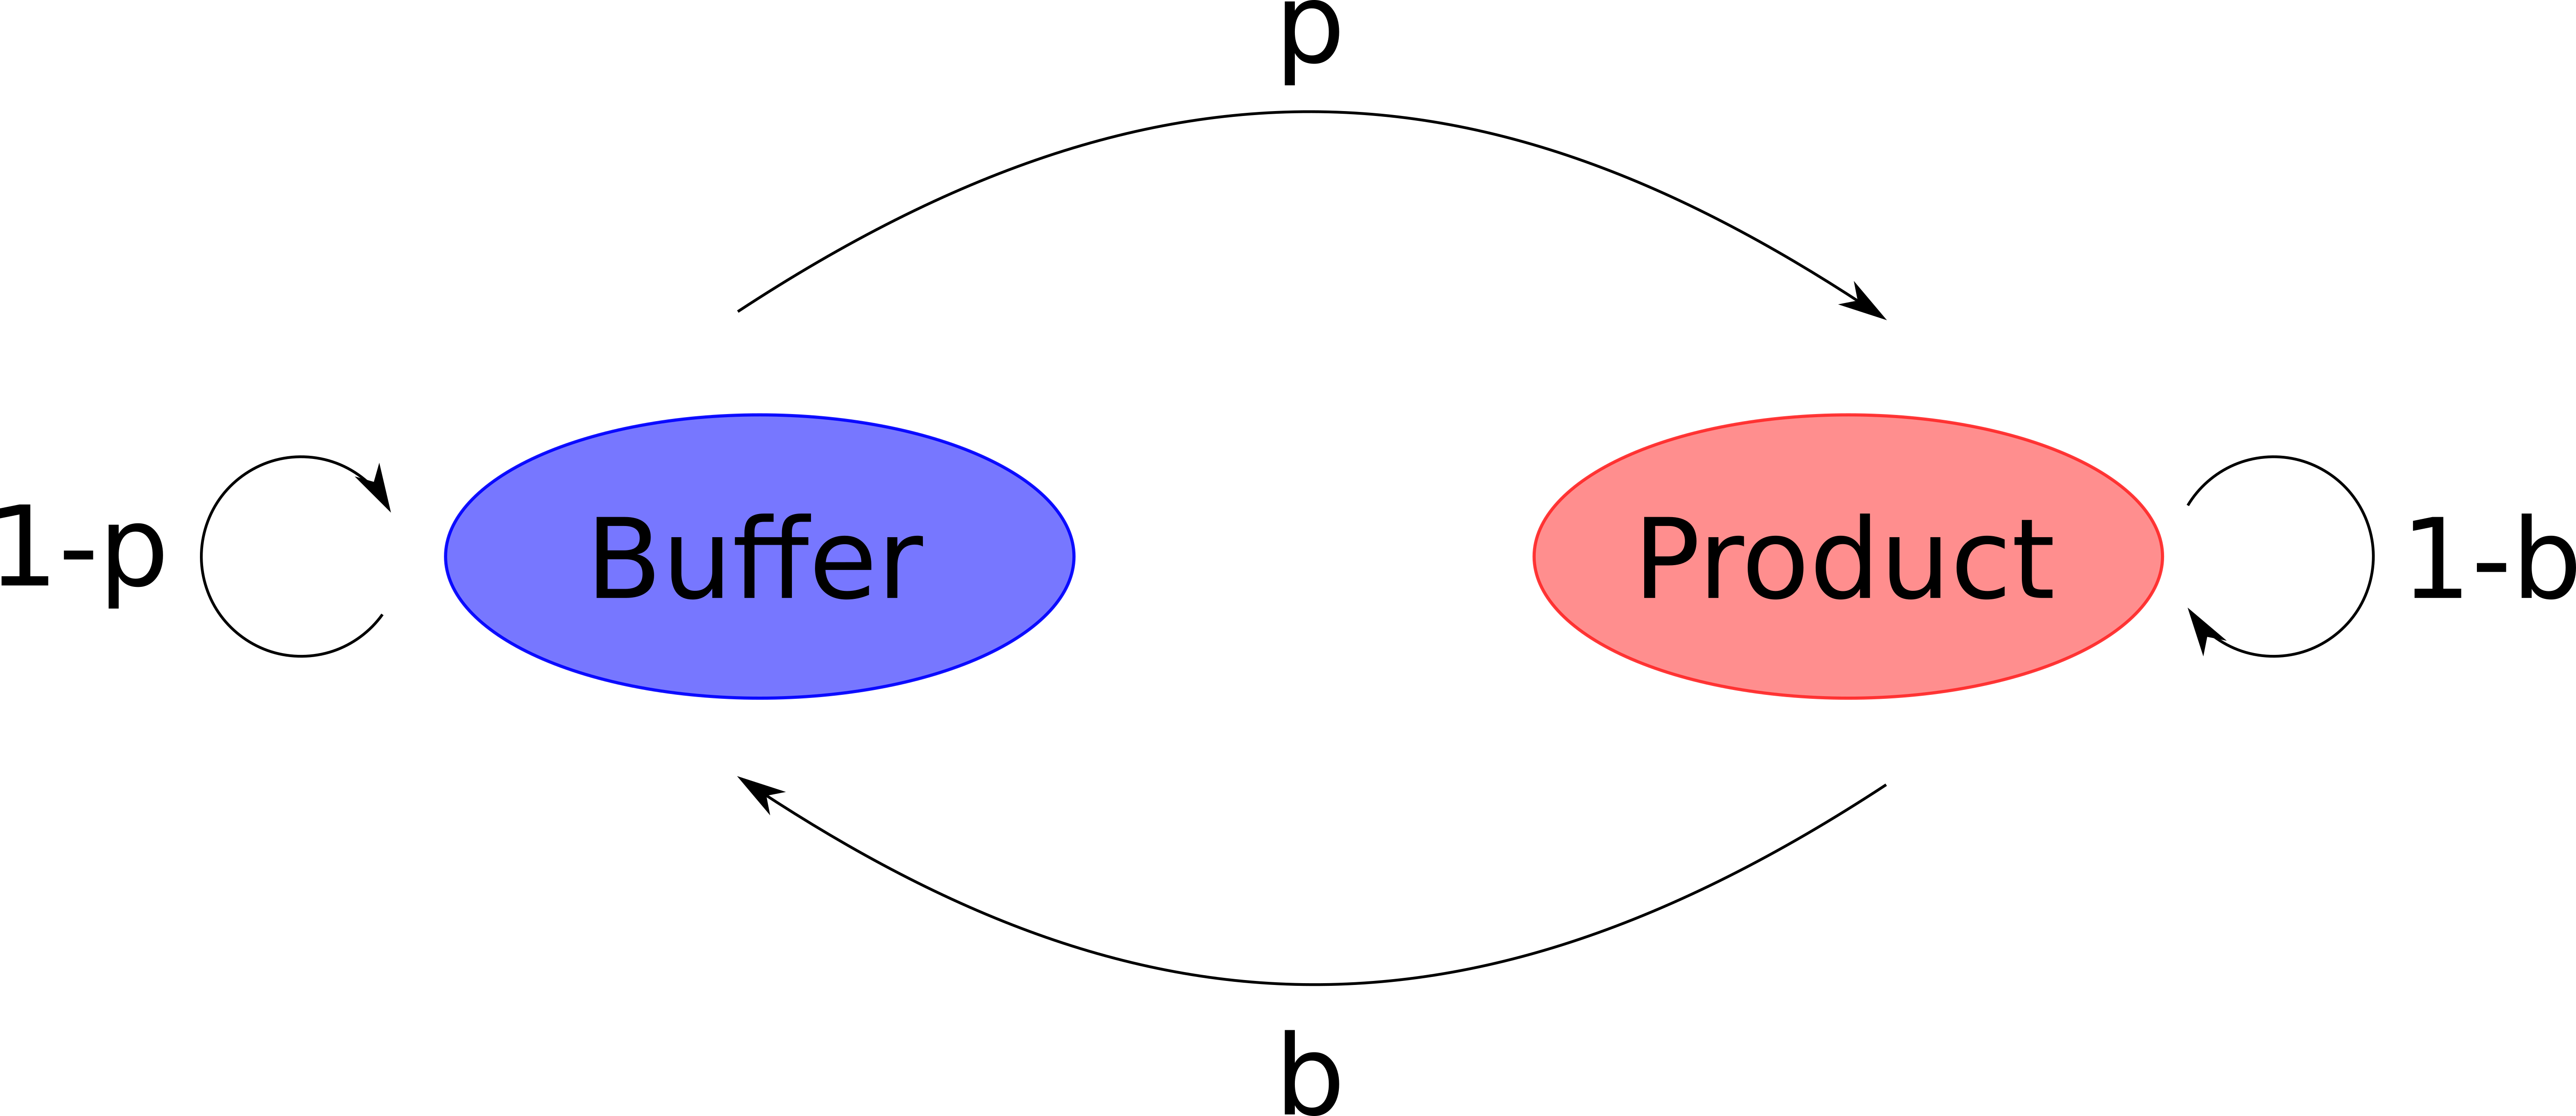
\includegraphics[width=0.85\textwidth]{part_2/assets/model.png}
    \caption{\textbf{Two states Markov chain model}}
    \label{markov_model}
  \end{figure}

  With this model, the preference index can be defined directly by $p-b$ the proportion of time spent in the product state minus the proportion of time spent in the buffer state. If $p$ (resp. $b$) can be defined, we take $PI=-1$ (resp. $PI=1$).

 An indicator of the fish exploration-exploitation behavior can be derived as follows:
$$ r_{markov} = 2Min(p,b) - 1 $$

  We can build a numerical simulation of two states Markov chain to explore the relationship between $p$ and $b$ probabilities, the preference index, and $r_{markov}$. The numerical simulation will construct Markov chain of probabilities $p$, and $b$. The length of the chain is drawn from the experimental chain length distribution that follows a discrete negative binomial distribution (see Figure~\ref{chain_fit}):
  $$
  f(k) = \begin{pmatrix}
  k+n-1\\
  n-1
  \end{pmatrix}
  a^n(1-a)^k
  $$
  \noindent With $n=2.527$ et $a=0.084$.

  \begin{figure}[h]
    \centering
    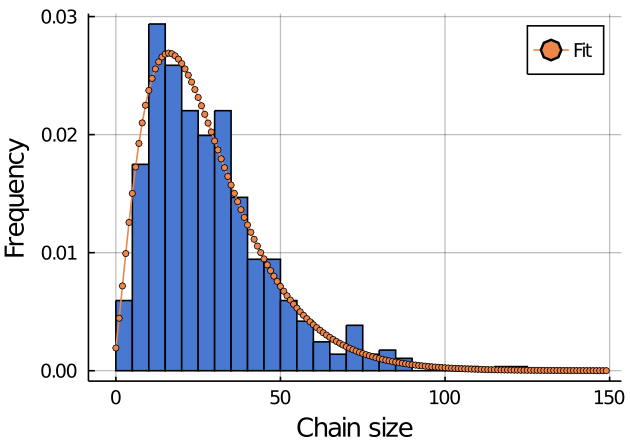
\includegraphics[width=0.65\textwidth]{part_2/assets/chain_fit.png}
    \caption{\textbf{Chain length} Chains length distribution.}
    \label{chain_fit}
  \end{figure}

  \begin{figure}[h]
    \centering
    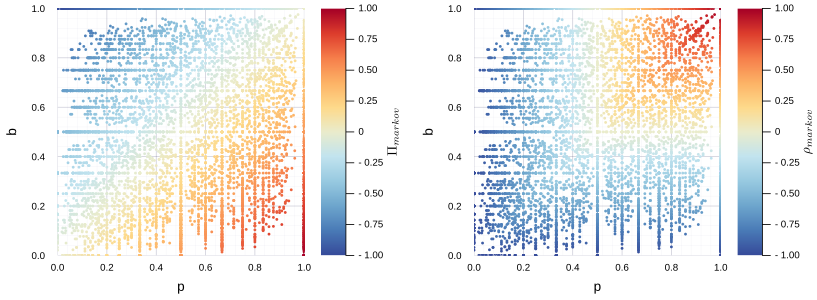
\includegraphics[width=0.85\textwidth]{part_2/assets/pi_pb.png}
    \caption{\textbf{Numerical simulation} Preference index and$r_{markov}$ for 10 000 realisations with a chain size following the experimental distribution.}
    \label{markov_simu}
  \end{figure}

  We see on Figure~\ref{markov_simu} that there are forbidden couples of $(p,b)$ due to the chain length. The preference indexes are distributed on either side of the identity line $p=b$ where $pi = 0$ with an upper triangle repulsive and a lower triangle attractive. Looking at the map of $r_{markov}$, we see a right upper corner at high $p$ and $b$ dominated by exploration, and a bottom left corner by exploitation. As expected, the fish can have a neutral preference with either exploration or exploitation, but a strong preference can only happen in a regime dominated by exploitation.

  \section{Results}
  \subsection{Setup caracterisation}
  \paragraph{Left-right bias} We started by checking the preference index in the B1 buffer cycle to capture an eventual left-right bias of setup. There is water on the two sides in this control cycle, and fish were never exposed to any product. We compute the time-based preference index choosing the middle of the tank as left-right separation (in B1, there is no dye, thus no real separation). Figure~\ref{ld_bias} presents the distribution of preference index for B1 cycles for larvae and juveniles. The first thing we can notice is the significant variability among fish. The median value ($pi = 0.08$ for $N=125$ for larvae and $pi = 0.05$ for $N = 178$ juveniles) is close to zero that will exclude any systematic left-right bias of the setup.

    \begin{figure}[h]
      \centering
      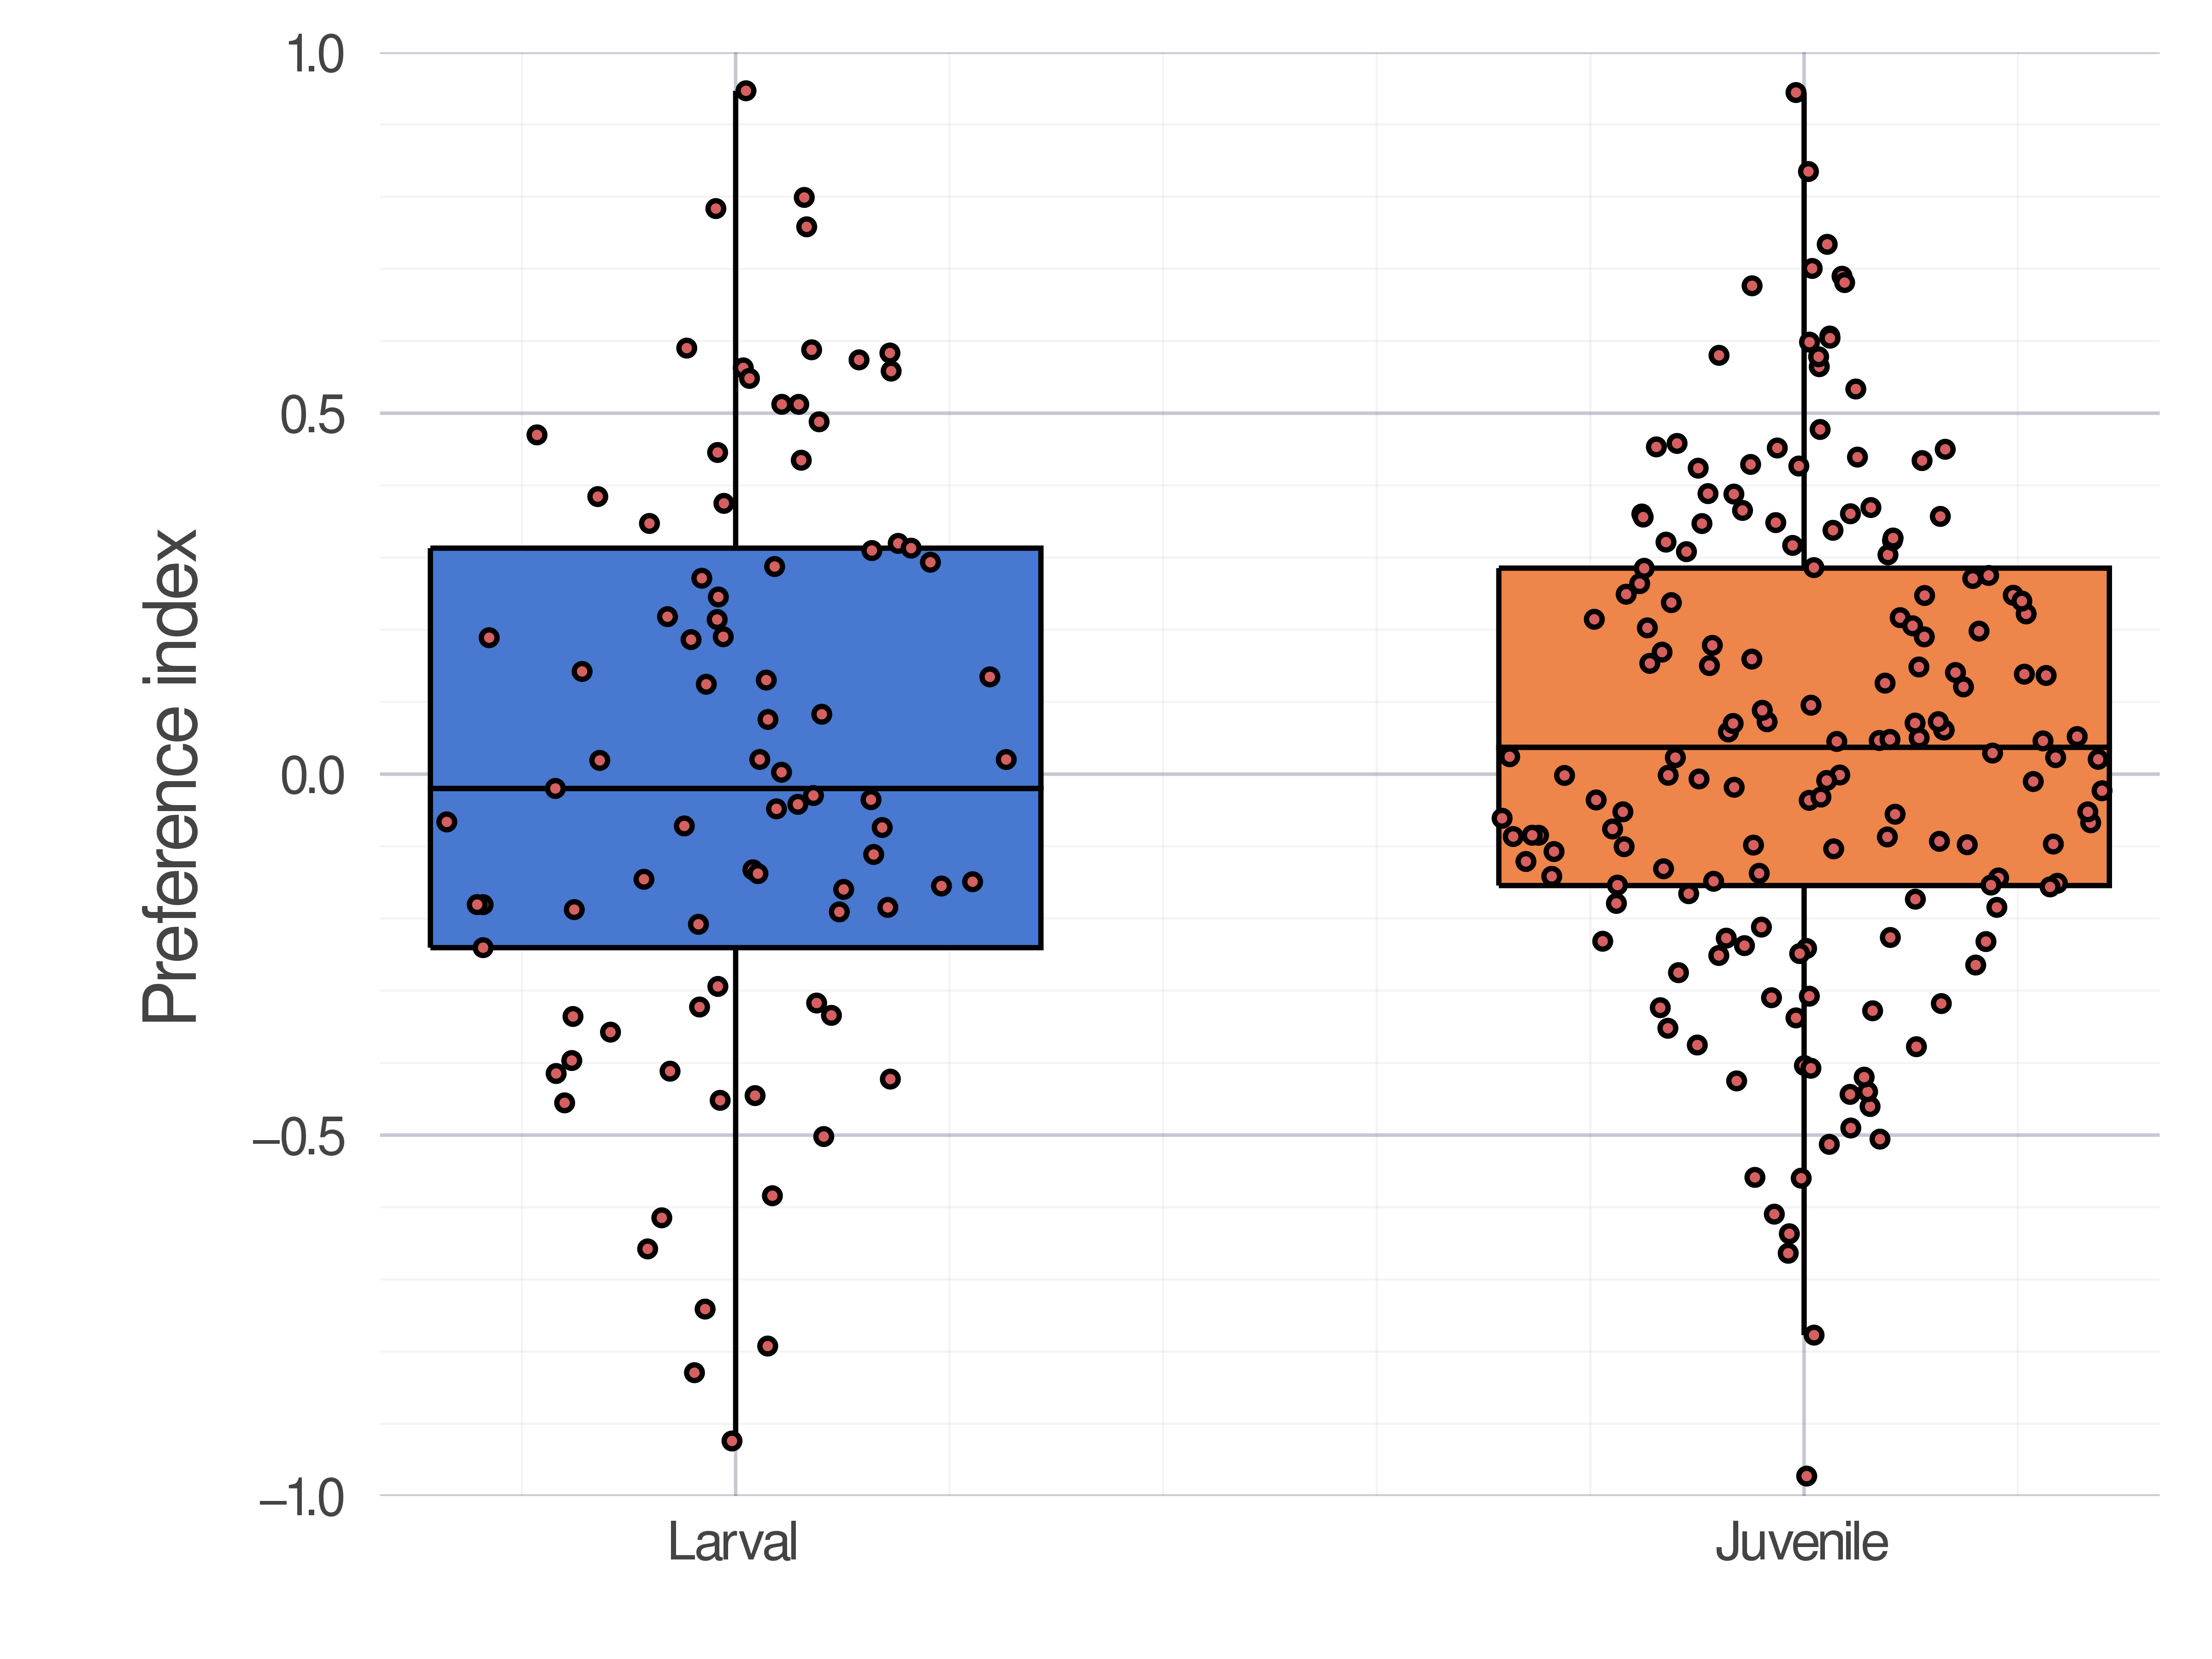
\includegraphics[width=0.75\textwidth]{part_2/assets/ld_bias.png}
      \caption{\textbf{Left-right bias} Distribution of the time preference index computed for the first buffer cycle (B1) with water on the two sides. Each point is a value of preference index for one fish. Black line is the distribution median.}
      \label{ld_bias}
    \end{figure}

  \paragraph{Dye neutrality} In the product cycles P1 and P2, the dye is diluted with the product to visualize the flow. To study the dye's impact on the fish, we performed control experiments with juvenile fish assessing only the dye with the protocol presented above.

  Figure~\ref{dye_bias}A presents the event-based preference index for the dye only. Each point is a fish for one independent manual analysis; the point's size encodes the number of events during the cycle. We see that the dye seems neutral to the fish with no clear attraction or repulsion. As expected, there is large inter-fish variability. The preference index distributions for P1 and P2 are not statistically significant, but cycle P2 includes more outliers fish with strong preferences.

  Figure~\ref{dye_bias}B presents the time-based preference index, each point representing one fish. We see a slight repulsion in the P1 cycle and a slight attraction in the P2 cycle toward the dye; there is no clear, robust preference toward the dye. These slight preferences are not visible with the event-based analysis and come from the time-based method that is less precise with our low statistics $N=13$ and more sensible to periods where the fish do not make a decision.

  Figure~\ref{dye_bias}C presents the $p$ and $b$ probabilities from the Markov chain model by fish. In each cycle, we see that $p \approx b \approx 0.65$, meaning that the fish can perceive the dye ($ p = b = 1$ mean that the fish do not perceive the dye) or at least the side change by another unknown mean. This effect is also visible on the ratio exploration-exploitation (Figure~\ref{dye_bias}D).

  Altogether, these results indicate that the fish can sense the dye but without manifesting any preference. With enough statistics to mitigate the fish inter-variability, we will be able to assess the fish preference while visualizing precisely the flow.

    \begin{figure}[H]
      \centering
      \includegraphics[width=0.75\textwidth]{part_2/assets/dye_pi.png}
      \caption{\textbf{Dye bias} \textbf{A.} Event-based preference index, one point is representing one fish for one independant analysis. \textbf{B.} Time-based preference index, one point is one fish. \textbf{C.} $p$ and $b$ probabilities from the Markov chain model, one point is representing one fish for one independant analysis. \textbf{D.} Ratio exploration-exploitation, one point is representing one fish for one independant analysis.}
      \label{dye_bias}
    \end{figure}

  \subsection{Products screening}
  We have screened several products known to elicit an aversion or attraction to the zebrafish. Because the literature is mainly focused on adult fish, our strategy was to assess early juvenile fish preference first and then reduce fish age.

  \paragraph{Citric acid juvenile}
  Citric acid is known to be repulsive in many fish species. It was shown that zebrafish could sense their environment pH \cite{abreu2016acute, abreu2016behavioral} and display a strong aversion for acidic pH ($pH \approx 3$). As a positive control, early juveniles and larval zebrafish preference were assessed using citric acid solutions ranging from $5 \times 10^{-3} M$ to $1 \times 10^{-6} M$, ie pH from $2.8$ to $4.2$ (Figure~\ref{citric_acid}).
    \begin{figure}[h!]
      \centering
      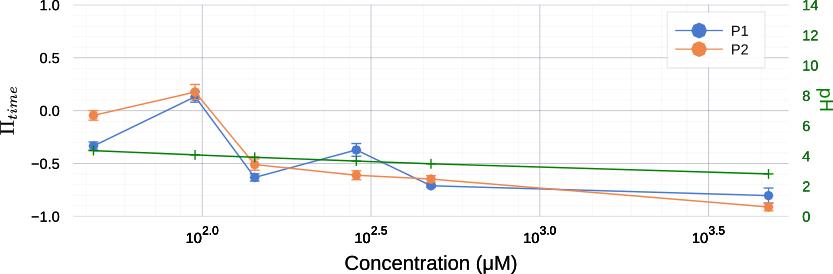
\includegraphics[width=.6\textwidth]{part_2/assets/citricacid.png}
      \caption{\textbf{Citric acid: time-based preference index} Time based preference index for P1 and P2 cycle (mean $\pm$ SEM), pH in green. }
      \label{citric_acid}
    \end{figure}
    \begin{figure}[h!]
      \centering
      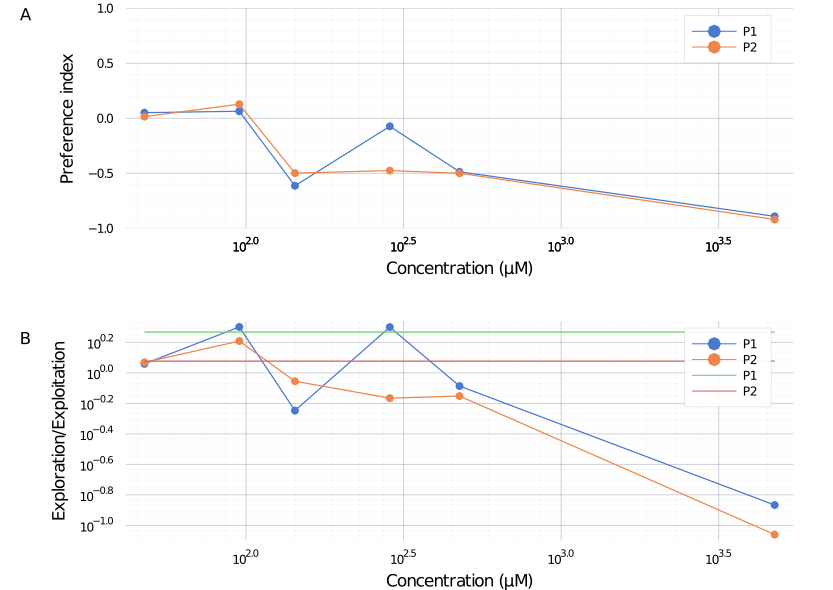
\includegraphics[width=0.8\textwidth]{part_2/assets/citricacid_event.png}
      \caption{\textbf{Citric acid: event-based analysis} A. Mean event-based preference index. B. Mean ratio exploration-exploitation.}
      \label{citric_acid_event}
    \end{figure}

  The ratio exploration-exploitation (Figures~\ref{citric_acid_event}B~\ref{citric_acid_markov}B) showed an apparent decrease when the citric acid concentration increase. Fish can sense citric acid and reduce their exploration to the benefit of a stereotyped exploitation behavior where they often go to the interface and return in the buffer (see Appendix~\ref{touch-turn} for a detailed description).

  The time-based (Figure~\ref{citric_acid}A), event-based (Figure~\ref{citric_acid_markov}B) and model-based (Figure~\ref{citric_acid}A) mean preference indexes decrease in a concentration-dependent manner. The distributions of preference indexes by fish (Figure~\ref{dist_citric_acid}) show a decrease in variability as the concentration increase and no significant difference between P1 and P2 cycles, which tends to suggest that fish adopt the same characteristic behavior with less variability as a preference emerged.

  \paragraph{Citric acid larvae} Preliminary experiments were done to assess the effect of citric acid on zebrafish larvae (Figure~\ref{dist_citric_acid}). Despite low statistics (see section\ref{discussion}) and significant variability, we see that citric acid seems to be repulsive as expected from juvenile results. More experiments need to be done to confirm this effect and account for the larvae inter-variability.
    \begin{figure}[h!]
      \centering
      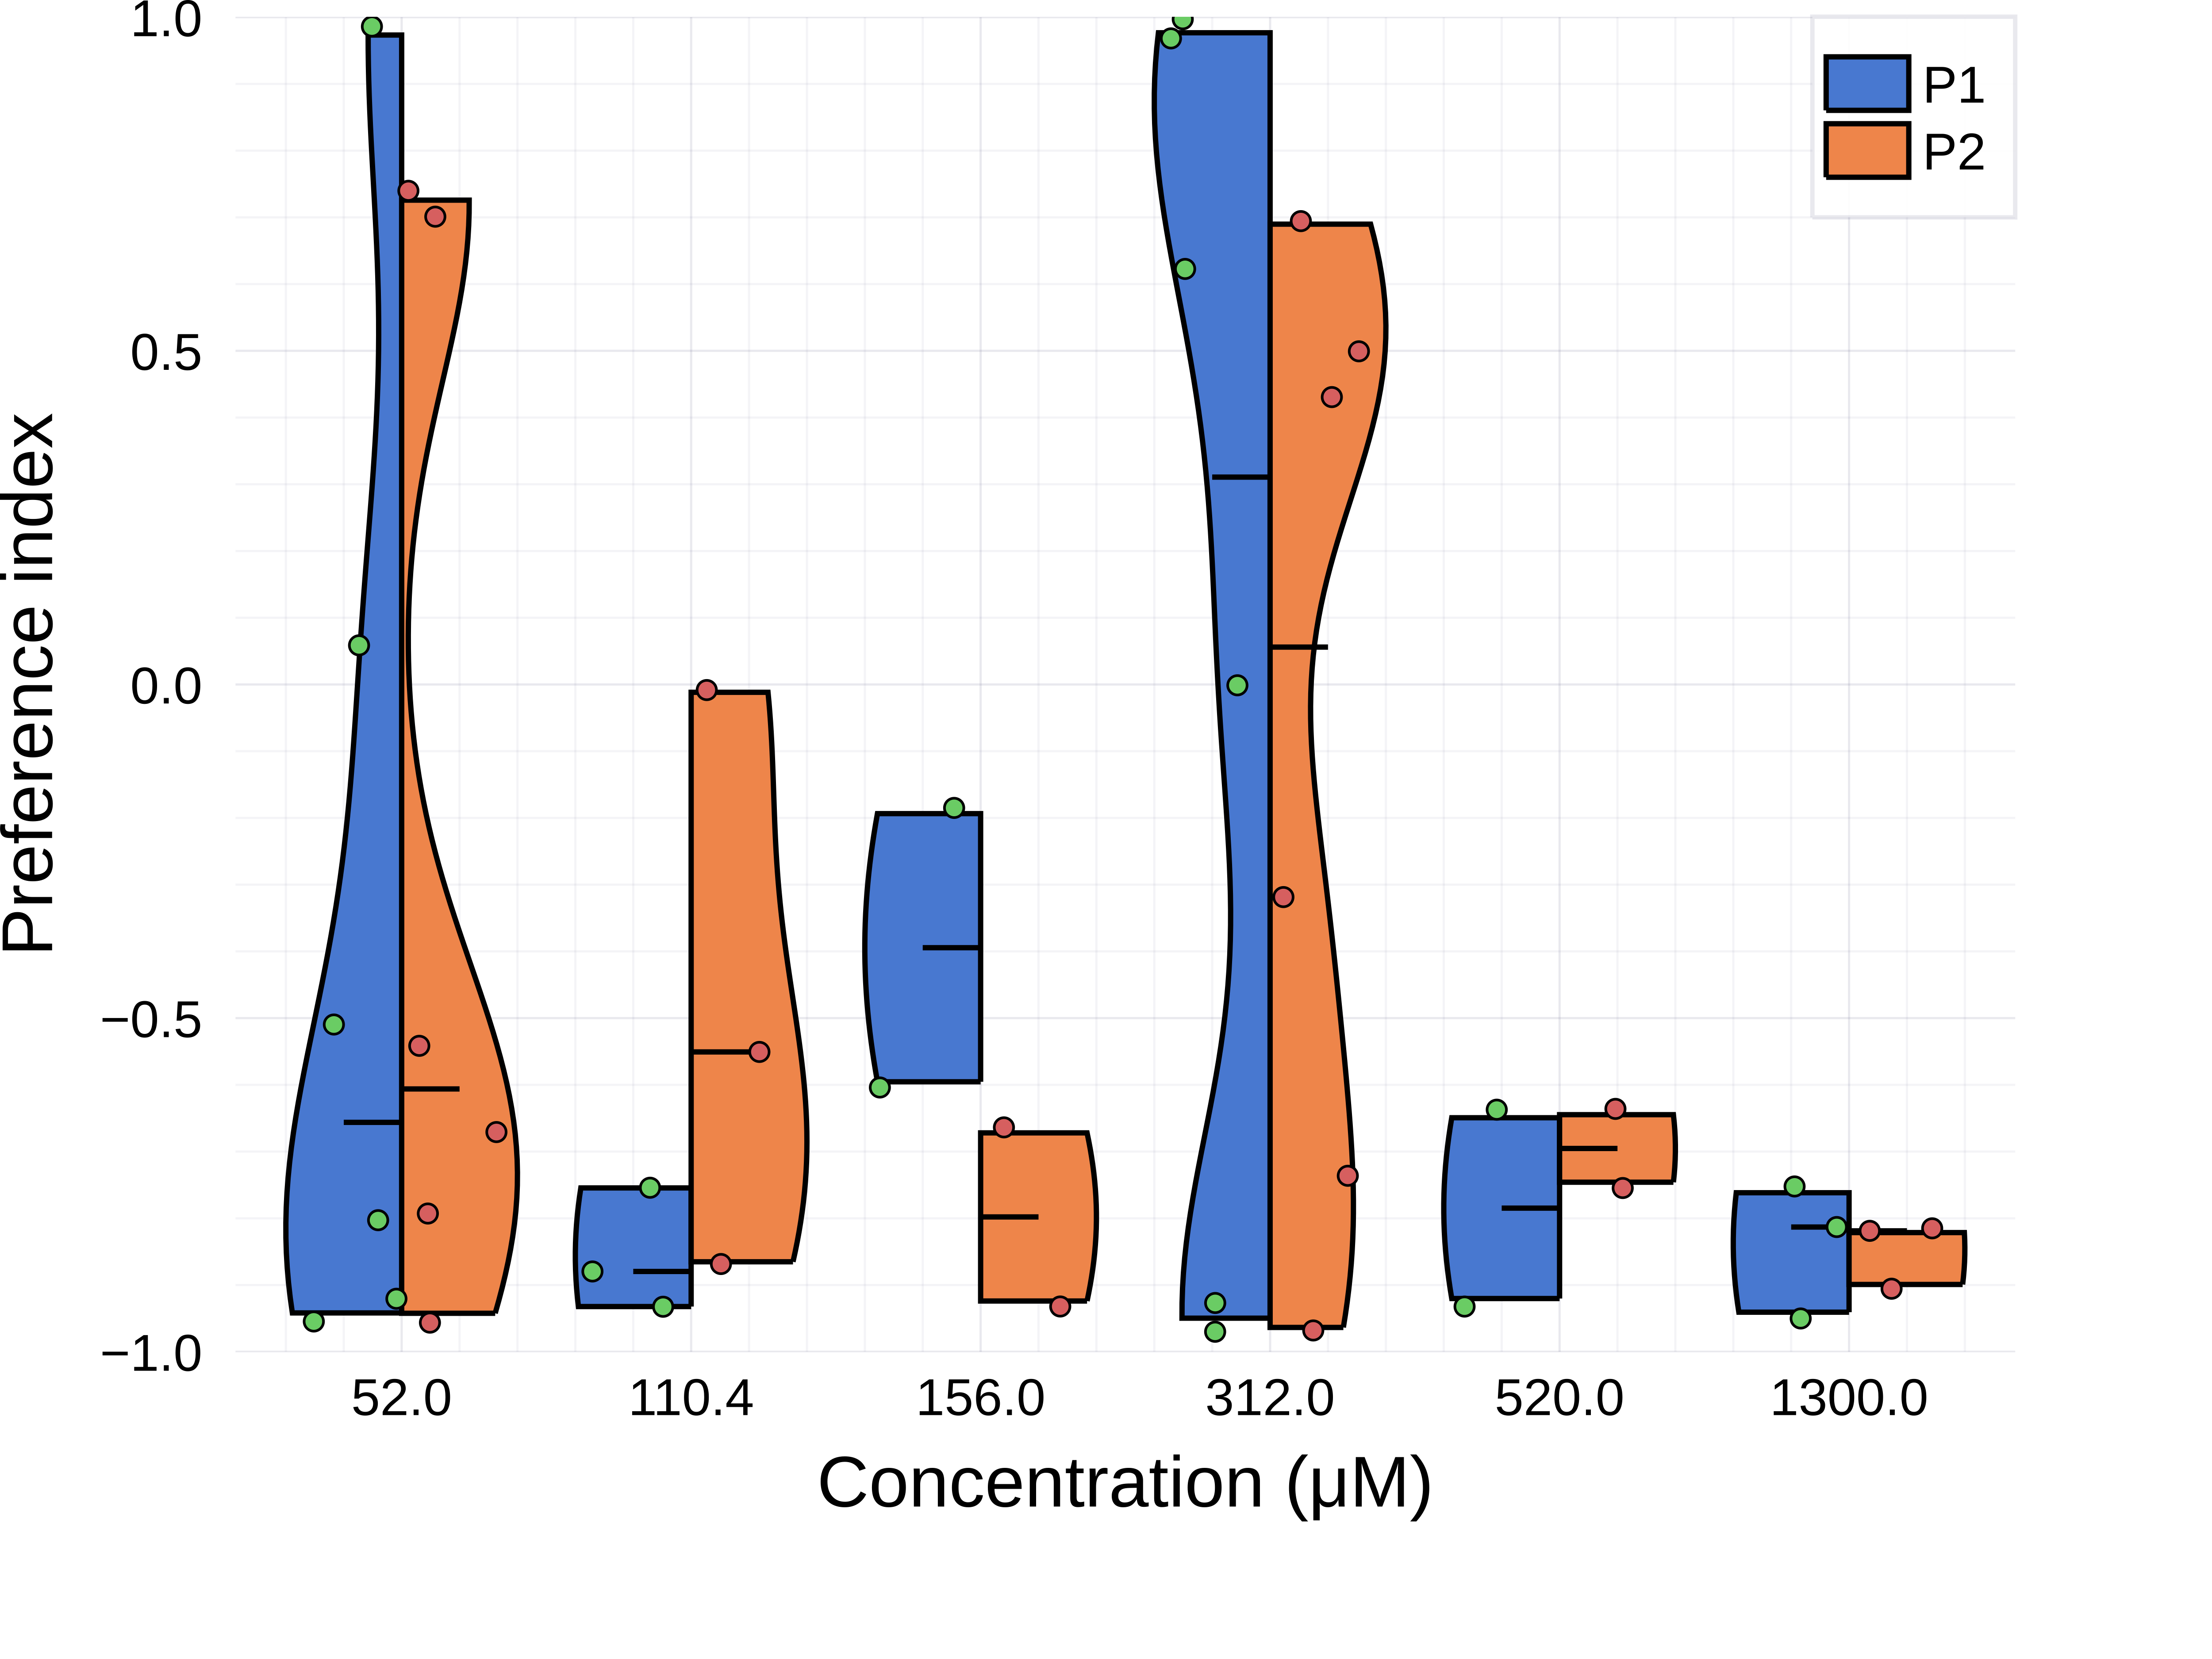
\includegraphics[width=0.8\textwidth]{part_2/assets/dist_citricacid_lar.png}
      \caption{\textbf{Citric acid: preference index for larvae} Time-based preference index, one point is one fish.}
      \label{dist_citric_acid}
    \end{figure}

  Using Dual, we were able to assess the repulsion to citric acid by zebrafish. Our analysis and model were able to capture the fish behavior changes and quantify the repulsion magnitude. As expected, the inter-fish variability is large but seems to be reduced by aversion where fish adopt a stereotyped exploitation behavior.

  \paragraph{ATP and adenosine}
  Zebrafish have pear-shaped olfactory sensory neurons expressing olfactory receptors specific to adenosine \cite{wakisaka2017adenosine}. ATP, ADP, and AMP are dephosphorylated in the zebrafish olfactory epithelium by two kinases \cite{wakisaka2017adenosine}. Behavioral responses to adenosine and ATP were shown to exist with arousal and food-seeking behavior. We assessed preference for ATP and adenosine for larval and early juveniles zebrafish. Fish were starved 24 hours before the experiment, and preference was assessed using the protocol presented below.

  \paragraph{Adenosine juveniles} Fish can perceive adenosine as indicated by the ratio exploration-exploitation (Figures~\ref{adenosine_event}B~\ref{adenosine_markov}B) that decrease with the concentration and are lower than the control (only dye).

  The event-based and model-based preference indexes (Figures~\ref{adenosine_event}A~\ref{adenosine_markov}A) show a slight repulsion for the P1 cycle and a slight attraction for the P2 cycle at the two lower concentrations.  The time-based preference index (Figures~\ref{adenosine}) displays a slight repulsive preference for the P1 cycle. There is no clear preference, and analysis from event-based and time-based preferences disagree, meaning that there is probably not enough statistic to conclude. Besides, preference index distributions (Figure~\ref{dist_adenosine}) show great variability.
    \begin{figure}[h!]
      \centering
      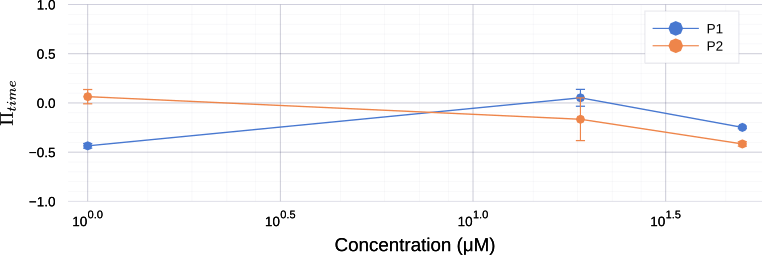
\includegraphics[width=0.6\textwidth]{part_2/assets/adenosine.png}
      \caption{\textbf{Adenosine: time-based preference index.} Time based preference index for P1 and P2 cycle (mean $\pm$ SEM).}
      \label{adenosine}
    \end{figure}
As no clear preference emerged from the early experiments, we focused on the concentration $50 \mu M$ and increased the statistics up to $N=28$. We see a slight repulsion on the P1 cycle at the same level that the other concentration. However, the P2 cycle shows a clear repulsion with a median preference index equal to $-0.6$ and 2 clusters of fish, one attracted and one repulsed.
    \begin{figure}[h!]
      \centering
      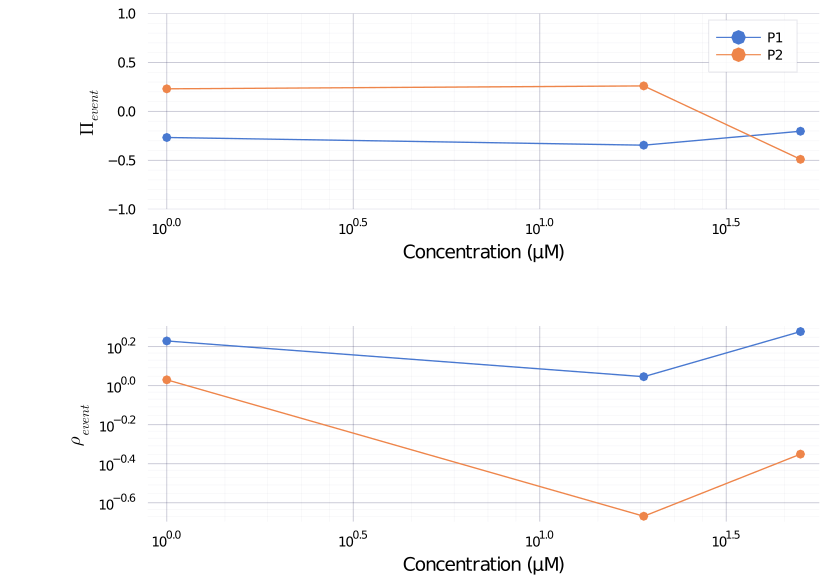
\includegraphics[width=0.8\textwidth]{part_2/assets/adenosine_event.png}
      \caption{\textbf{Adenosine: event-based analysis} A. Mean event-based preference index. B. Mean ratio exploration-exploitation.}
      \label{adenosine_event}
    \end{figure}
  Unexpectedly, adenosine does not seem to attract early juvenile zebrafish. On the contrary, at high concentration, it is clearly repulsive. However, one part of the fish ($\approx 30 \%$) seems to be either attracted or neutral at the second presentation of the product.

    \paragraph{Adenosine larvae} Zebrafish larvae were exposed to adenosine with the same protocol as juveniles. Preliminary results (Figure~\ref{dist_adenosine_lar}) based on the time preference index seems to indicate no strong preference at any concentration.
  \begin{figure}[h!]
      \centering
      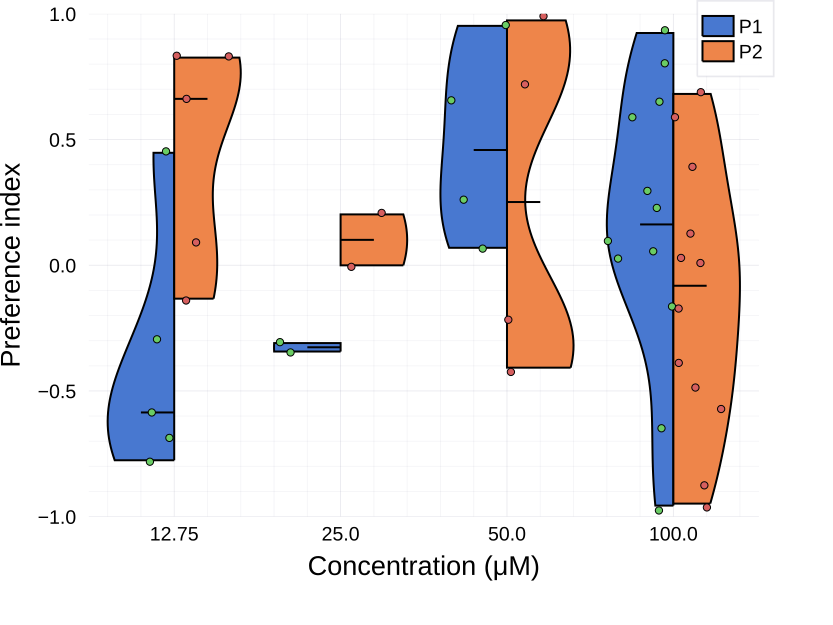
\includegraphics[width=0.8\textwidth]{part_2/assets/dist_adenosine_lar.png}
      \caption{\textbf{Adenosine: preference index for larvae} Time-based preference index. One point is one fish, black line is the distribution median.}
      \label{dist_adenosine_lar}
    \end{figure}

  \paragraph{ATP juveniles} Interestingly, we find that ATP, a product that was shown to be attractive on adults, produces a two phases behavior on early juvenile zebrafish (Figures~\ref{atp}A~\ref{atp_event}A~\ref{atp_markov}A). At low concentration, fish do not manifest a preference, but at the highest concentration ($125 \mu  M$  and $200 \mu M$), the P1 cycle became repulsive and the P2 cycle attractive.
    \begin{figure}[h!]
      \centering
      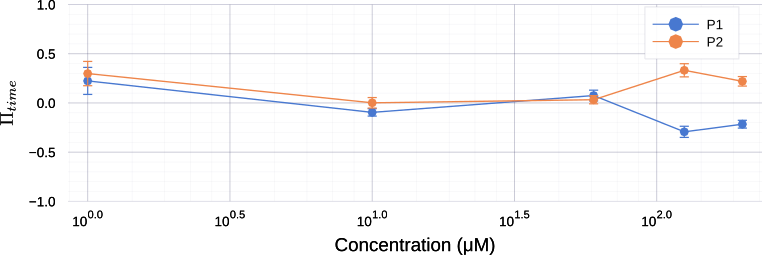
\includegraphics[width=0.6\textwidth]{part_2/assets/atp.png}
      \caption{\textbf{ATP: time-based preference index.} }
      \label{atp}
    \end{figure}
  Comparing the distribution of event-based and time-based preference index by fish (Figure~\ref{dist_atp}), we see that this effect is significant at $125 \mu M$ and  $200 \mu M$ (one-sided Wilcoxon signed-rank test).
    \begin{figure}[h!]
      \centering
      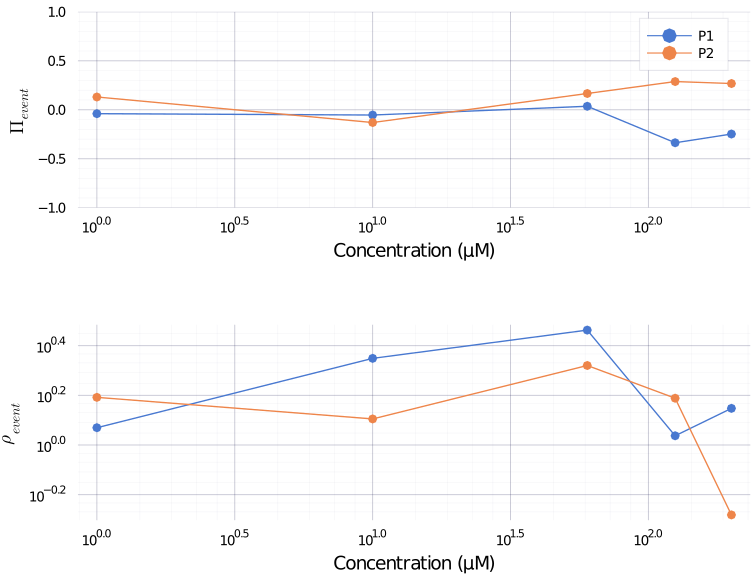
\includegraphics[width=0.8\textwidth]{part_2/assets/atp_event.png}
      \caption{\textbf{ATP: event-based analysis} A. Mean event-based preference index. B. Mean ratio exploration-exploitation.}
      \label{atp_event}
    \end{figure}
  A fish by fish analysis (Figure~\ref{proportion}A) reveals that the fish proportion that changes its preference toward attraction increase with the concentration. (Figure~\ref{proportion}B) represents the $p$ and $b$ probability from the markov chain model. We can see that a lot of fish cross the identity line between the P1 and P2 cycle to invert their preference indexes.
    \begin{figure}[h!]
      \centering
      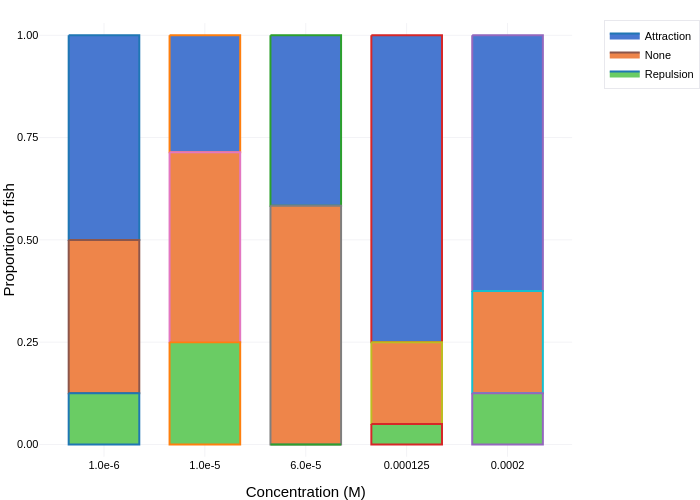
\includegraphics[width=0.8\textwidth]{part_2/assets/proportion.png}
      \caption{\textbf{Cycle effect} \textbf{A}. Fish proportion changing preference between the P1 and P2 cycles. \textbf{B}. Probabilities $p$ and $b$ for $125$ and $200 \mu M$, one point is one fish for one independent analysis ($2N$ fish).}
      \label{proportion}
    \end{figure}

    \paragraph{ATP larvae} Zebrafish larvae were exposed to ATP with the same protocol as juveniles. Preliminary results (Figure~\ref{dist_atp_lar}) based on the time preference index indicate a repulsion at every concentrations. High concentrations seem to produce more robust repulsive behavior with low variability.

    \begin{figure}[h!]
      \centering
      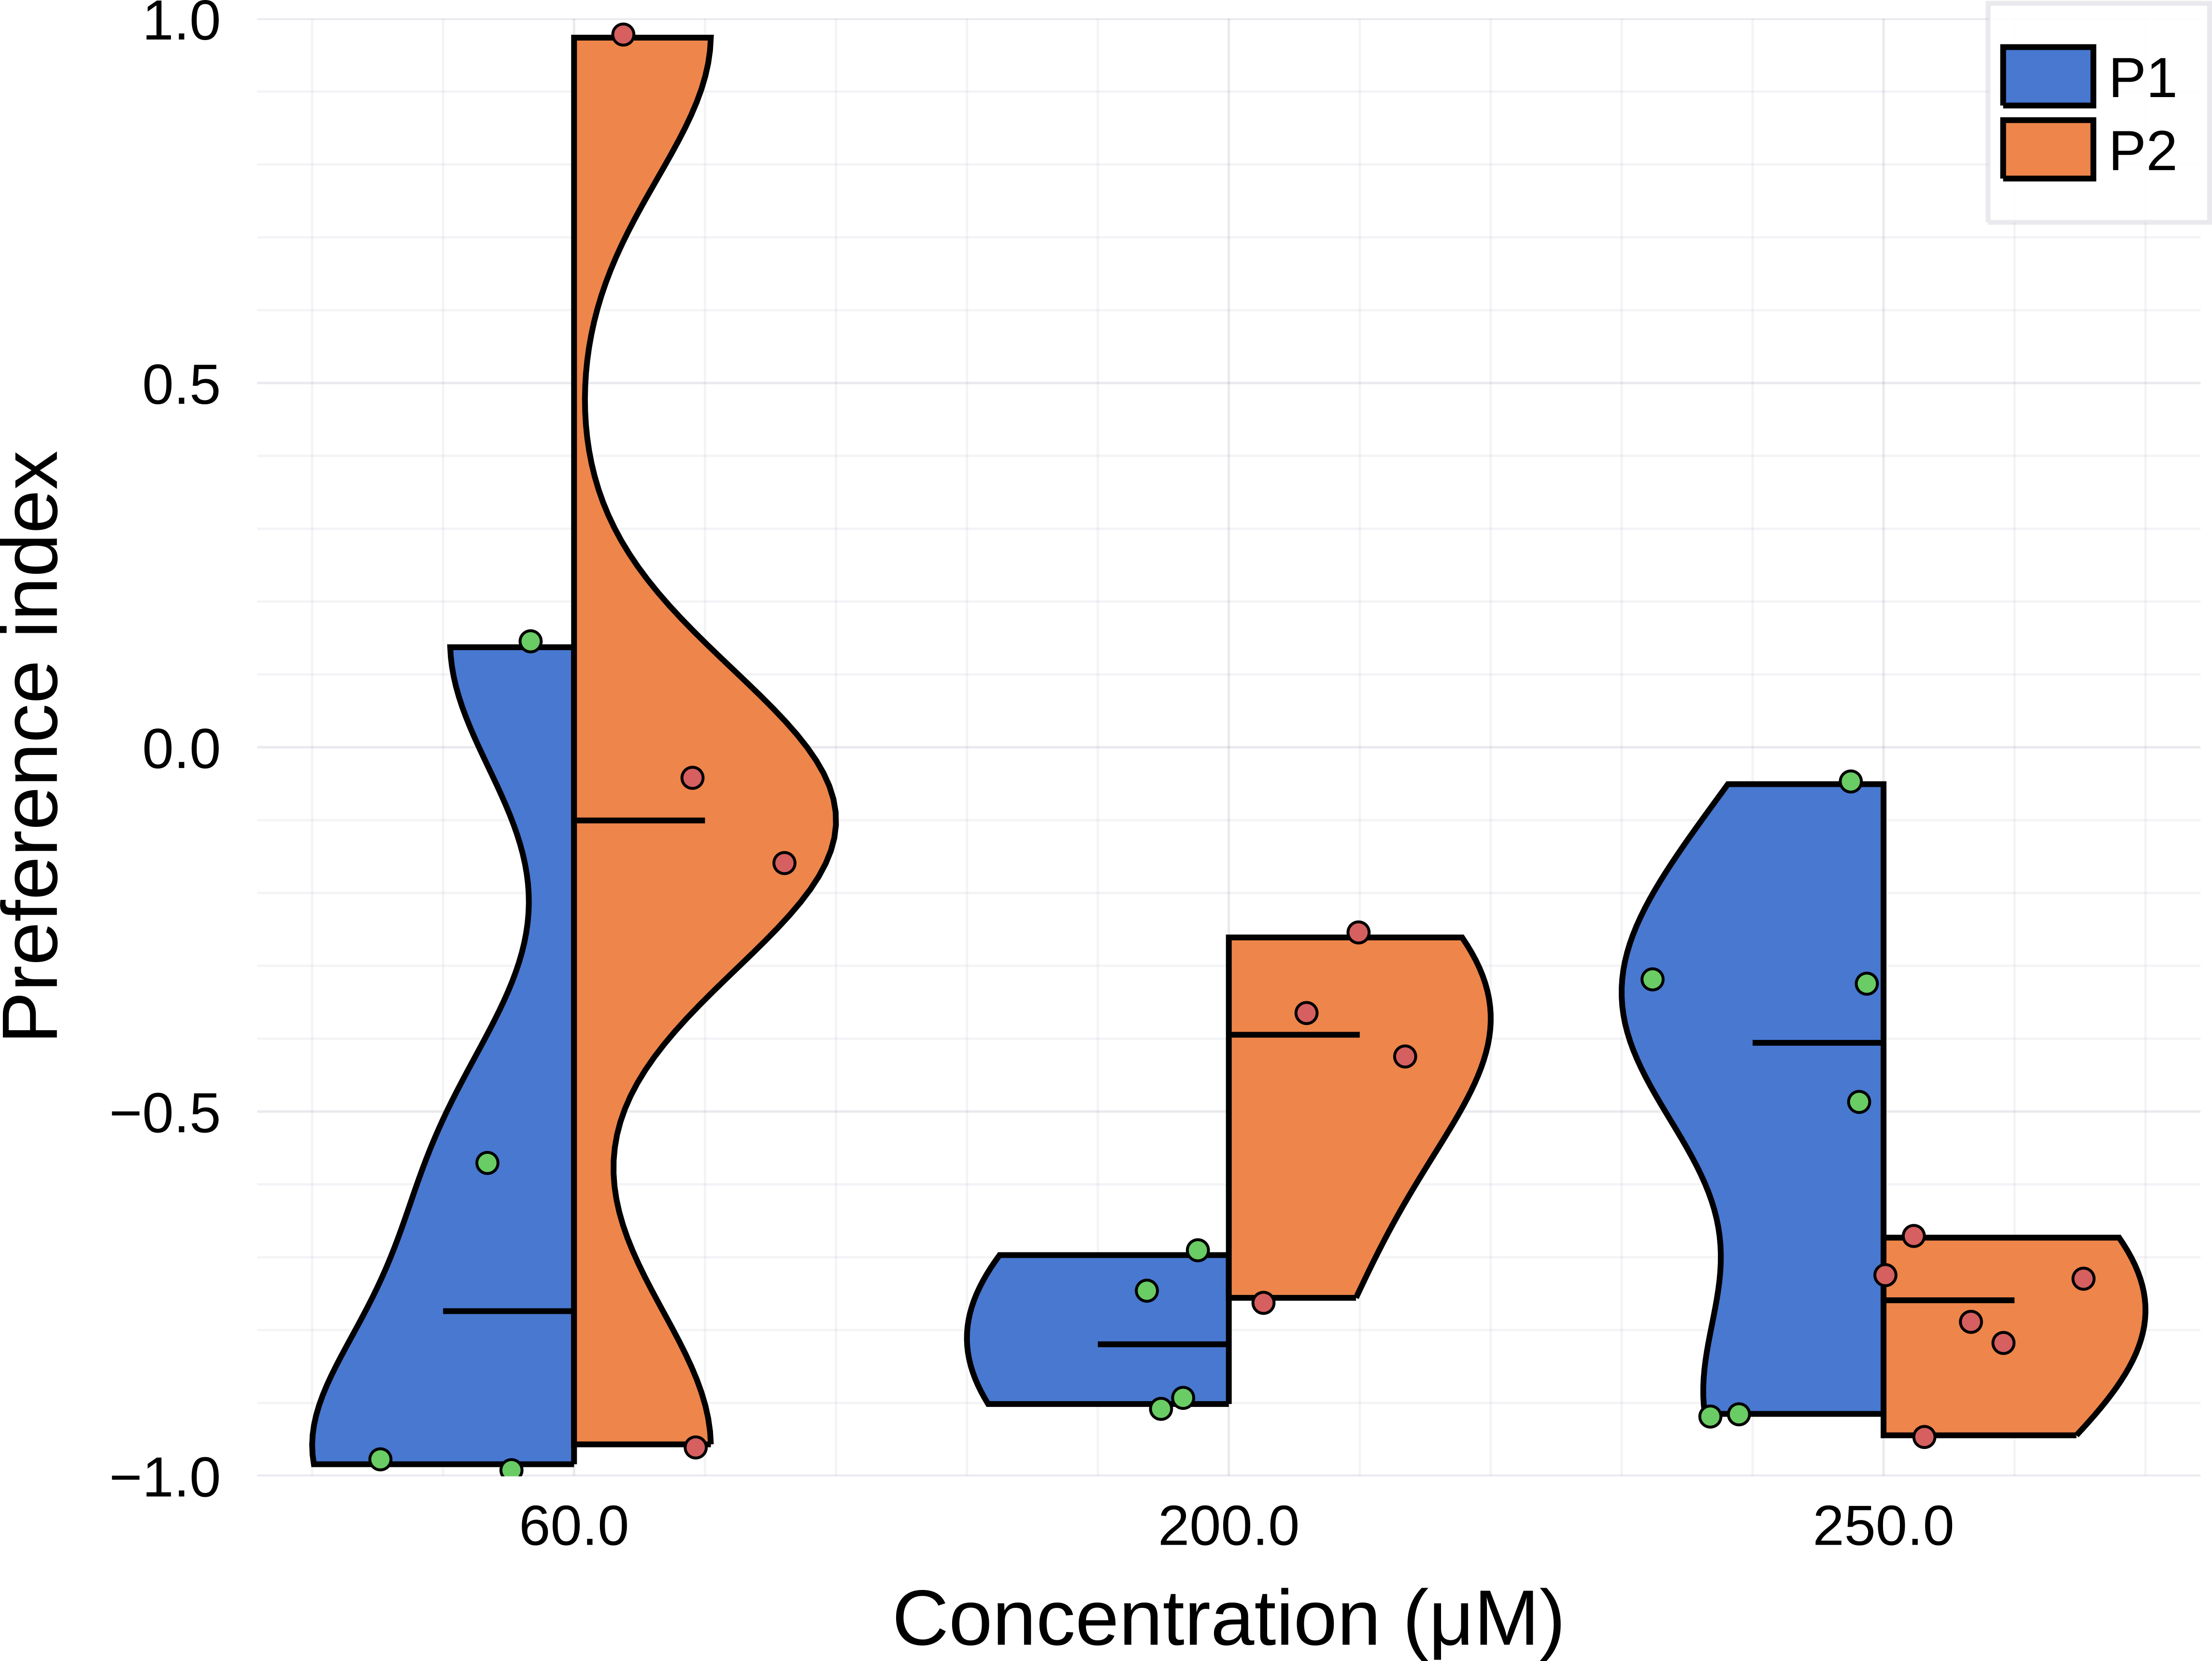
\includegraphics[width=0.8\textwidth]{part_2/assets/dist_atp_lar.png}
      \caption{\textbf{ATP: preference index for larvae} Time-based preference index. }
      \label{dist_atp}
    \end{figure}

  Not documented in the literature to our knowledge, an interesting effect was found on juvenile zebrafish exposed to ATP with an inversion of preference at the second product presentation. Experiments with larvae do not seem to indicate the same effect. More experiments need to be done, especially on larvae and at intermediate ages, to better characterize this behavior.

    \paragraph{Quinine juveniles} Quinine is a natural alkaloid that tastes bitter, and that is a highly deterrent substance for many fish species \cite{kasumyan2003taste}. Unexpectedly, we see with the time-based preference index (Figure~\ref{dist_quinine}) that the preference seems to be mostly neutral. A slight attraction can be constated on the P1 cycle, and a neutral a slightly repulsive preference on the P2 cycle. Despite relatively good statistics ($\approx 7$ fish by concentration), no robust preference emerged as we see with a large variability in responses.
    \begin{figure}[h!]
      \centering
      \includegraphics[width=0.8\textwidth]{part_2/assets/dist_quinine.png}
      \caption{\textbf{Quinine: preference index for juveniles} Time-based preference index. One point is one fish. }
      \label{dist_quinine}
    \end{figure}

  \chapter{Conclusion}
  \label{discussion}
  In these chapters, we saw how we built two experimental setups to assess and understand the chemical preference of larval and early-juveniles zebrafish.

  The Tropical River is a setup capable of producing controlled flows. The flow temperature and velocity can be precisely controlled. Turbulent and laminar jets can be created inside the flow to mimic more realistic fragmented chemical perception. This setup was originally developed to study the chemically-driven navigation after finding a robust, attractive compound with Dual. Due to the difficulty of finding such a product, we could not use it in the context of this project. Nonetheless, several preliminary experiments were performed to check the setup, and it was used in another project to study the fish swimming taking advantage of the flow velocity control and high framerate imaging.

  Dual is a high-throughput chemical screening setup that allows exploring the combination of products, concentrations, and fish ages easily and rapidly. The setup is scalable and can be built at the laboratory for less than 1500 USD. In the first part of the thesis, we built the setup and controlled that it did not have any bias. We check that the infrared dye used to visualize the flow was neutral to the fish. We successfully use Dual to assess the chemical preference of several products. We show a strong aversion to citric acid and an exciting effect with ATP where fish inverts their preferences at the second product presentation. Work remains to be done to precisely characterize this effect. An interesting question would be to check what happened at the third presentation of ATP. It can be done easily by adding a cycle to the experiment. If this attractive preference persists in time, ATP could be used in The Tropical River to study chemically-driven navigation. A temporal characterization would also be of great interest. Adults were shown to be attracted by ATP without mention of prior exposures. Studying the effect at a fixed concentration, like $125 \mu M$, by varying the fish age will help understand the development of ATP's perception from larvae to adults.

  Preliminary results shown with larvae need more statistics. Studying larvae poses several challenges. First, larvae tend to explore less than juveniles, and combined with their small sizes, they do not frequently cross the interface. We circumvented this problem by putting up to 4 larvae by experiment, thus increasing the statistics, but this adds work in the analysis phase. Secondly, larvae are more susceptible to fatigue and freezing than juveniles. It frequently happens that larvae stop swimming and do not recover until the end of the experiment. For this reason, assessing the ATP effect on larvae is very challenging: reducing cycles length to reduce fatigue will lead to fewer crossing events, but longer cycles will lead to more fish dropouts before the cycle P2. For this reason, studying larvae will need many statistics, a thing that we had not the time to do in the context of this thesis.

  The analysis methods are fragmented according to fish ages and products. We first implemented a coarse-grained approach where we recorded the fish's position and computed the time-based preference index taking the mean interface position. Then we tried to refine this approach to better characterize the fish behavior at the interface by extracting the interface position. This was not practically achievable due to several constraints: time, fish complex behavior, and challenging image processing problems on a large amount of data (8 To of data). Finally, we chose to perform a manual analysis that focuses on events happening at the interface, moments where the fish had to make a decision. It was possible to confirm the time-based analysis results with this approach and characterize the fish behavior more precisely. This approach was only applied to products where there were enough statistics and already interesting effects to delve into.

 Studying the chemical perception of zebrafish proved to be challenging. The fish inter-variability is high, as we have seen by screening products. In these experiments, we use 4 Duals to record up to 350 hours of usable experiments, but we see that more statistics are needed. We hope that Dual as a low-cost, easily replicable setup will encourage people to build and use the setup to better characterize zebrafish chemo-preference.


\begin{appendices}

  \chapter{Dual bill of materials}
  \includepdf[pages=-]{part_2/assets/bom.pdf}
  \label{bom}

  \chapter{Visualisation}
    \section{Boxplot}
    The boxplot is a non-parametric method to represent data graphically using their quartiles, its read as indicated in the Figure~\ref{boxplot}.
      \begin{figure}[h]
        \centering
        \includegraphics[width=0.45\textwidth]{part_2/assets/boxplot.png}
        \caption{\textbf{Boxplot}}
        \label{boxplot}
      \end{figure}

    \section{Violinplot}
    The violinplot is a non-parametric method to represent data graphically using their kernel density plot, see Figure~\ref{violinplot}. The kernel density estimation is a non-parametric method to estimate the probability density function. The width kernel density plot will give the frequency of a given value.
      \begin{figure}[h]
        \centering
        \includegraphics[width=0.45\textwidth]{part_2/assets/violinplot.png}
        \caption{\textbf{Violinplot}}
        \label{violinplot}
      \end{figure}

  \chapter{Calculation}
    \section{Mean quantities}
    Mean quantities were calculated from events count following these definition:
    $$
    \bar{P}\bar{I} = \frac{\sum_{fish}^{}(n_{BP} + n_{PP} - n_{BB} - n_{PB})}{\sum_{fish}^{}(n_{BP} + n_{PP} + n_{BB} + n_{PB})}
    $$
    $$
    \bar{r} =\frac{\sum_{fish}^{}(n_{BP} + n_{PB})}{\sum_{fish}^{}(n_{BB} + n_{PP})}
    $$
    $$
    \bar{p} = \frac{\sum_{fish}^{}n_{BP}}{\sum_{fish}^{}(n_{BP} + n_{BB})}
    $$
    $$
    \bar{b} = \frac{\sum_{fish}^{}n_{PB}}{\sum_{fish}^{}(n_{PB} + n_{PP})}
    $$

    \section{Statistical tests}
    Statistical significance was evaluated using the Wilcoxon signed-rank test, one-sided when knowing the effect's direction, or two-sided otherwise. In the case of the event-based analysis, the test was carried out separately on the two independent manual counting then averaged to avoid a size effect bias.

    \section{Image analysis}
    Fish head position was extracted using FastTrack. Each recording was manually checked to remove low-quality movies either with imperfect flows or non-responsive fish.

    A custom image processing procedure was developed to extract the interface using the contrast difference due to the dye see Figure~\ref{}. First, the maximal and minimal z-projection of the movie was calculated. For the minimal projection, the fish is masked with a white mask on each image before the projection, only keeping the flow and not projection the fish. Each image of the movie is then normalized with minimal and maximal projection. Finally, the interface was detected using an Otsu threshold.

    A python command-line interface \footnote{\url{https://github.com/LJPZebra/dual_analysis}} was created to export the relevant data in a synthetic toml file easy exportable, one experiment by file. Statistical analysis and numerical simulations were performed using Python and Julia programming language.

  \chapter{Markov Model}
    \begin{figure}[h]
      \centering
      \includegraphics[width=0.8\textwidth]{part_2/assets/citricacid_markov.png}
      \caption{\textbf{Citric acid: Markov chain analysis} \textbf{A}. Mean Markov chain preference index. \textbf{B}. Mean Markov chain ratio exploration-exploitation.}
      \label{citric_acid_markov}
    \end{figure}
    \begin{figure}[h]
      \centering
      \includegraphics[width=0.8\textwidth]{part_2/assets/adenosine_markov.png}
      \caption{\textbf{Adenosine: Markov chain analysis} \textbf{A}. Mean Markov chain preference index. \textbf{B}. Mean Markov chain ratio exploration-exploitation.}
      \label{adenosine_markov}
    \end{figure}
    \begin{figure}[h]
      \centering
      \includegraphics[width=0.8\textwidth]{part_2/assets/atp_markov.png}
      \caption{\textbf{ATP: Markov chain analysis} \textbf{A}. Mean Markov chain preference index. \textbf{B}. Mean Markov chain ratio exploration-exploitation.}
      \label{atp_markov}
    \end{figure}

  \chapter{Preference index distributions}
    \begin{figure}[h]
      \centering
      \includegraphics[width=1\textwidth]{part_2/assets/dist_acid.png}
      \caption{\textbf{Citric acid: preference index for juveniles} \textbf{A.} Event-based preference index, one point is one fish for one independent analysis (total of $2N$ points). \textbf{B.} Time-based preference index, one point is one fish. }
      \label{dist_citric_acid}
    \end{figure}
    \begin{figure}[h]
      \centering
      \includegraphics[width=1\textwidth]{part_2/assets/dist_adenosine.png}
      \caption{\textbf{Adenosine: preference index for juveniles} \textbf{A.} Event-based preference index, one point is one fish for one independent analysis (total of $2N$ points). \textbf{B.} Time-based preference index, one point is one fish. }
      \label{dist_adenosine}
    \end{figure}
    \begin{figure}[h]
      \centering
      \includegraphics[width=1\textwidth]{part_2/assets/dist_atp.png}
      \caption{\textbf{ATP: preference index for juveniles} \textbf{A.} \textbf{A.} Event-based preference index, one point is one fish for one independent analysis (total of $2N$ points). \textbf{B.} Time-based preference index, one point is one fish.  }
      \label{dist_atp}
    \end{figure}

\end{appendices}


\bibliography{biblio}
\bibliographystyle{abbrv}
\end{document}

